% !TEX root = ../main.tex

\glsresetall


\topquote[9cm]{
The first principle is that you must not fool yourself --\\
and you are the easiest person to fool.}
{Richard Feynman}

{
\singlespacing
\chapter{Consideration of genotype error in the inference of haplotype sharing by descent}
\label{ch:generr}
\minitoc
}


%
\section{Introduction}
%

Recent advancements in genotyping and \gls{ngs} technologies have enabled us to study the human genome in unprecedented detail and scale.
The availability of high-throughput methods to survey large samples has led to successful identification of thousands of disease causing risk factors, which in particular was driven by \gls{gwa} studies.
This explosion of human genetic data has further enabled collaboration initiatives through the setup of genetic databases, which can be queried by research groups worldwide.
However, because no technology is perfect, acquired data are likely to contain undetected amounts of error, which may affect statistical inference in many ways.

Statistical tests often rely on the assumption that genotype data (retained after quality control) are correct, or that error quantities are negligible.
Yet, the effects of misclassification in genotype data are well documented.
For example, it has been shown that even minor amounts of genotype error can distort estimated distances in linkage mapping studies \citep{Buetow:1991wc,Shields:1991uw,Sobel:2002}, result in a substantial loss of linkage information in quantitative trait analyses \citep{Douglas:2000hb,Abecasis:2001jp}, decrease power in association studies \citep{Kang:2004hy}, and can substantially increase type I (false positive) error in haplotype-based case-control analyses \citep{moskvina2005minor}.

Identification of incorrectly typed or called genotypes remains a difficult problem, which becomes more challenging as the magnitude of data increases.
But, for example, as shown by \citet{Cox:2006kv} and independently by \citet{Moskvina:2006fz},
genotype error \Addition{theoretically} does not always affect the distributions of genotypes to the extent that \gls{hwe} can be violated.
\Correct{Given the common practise to exclude presumably incorrect genotypes based on departures from \gls{hwe}, it therefore remains difficult to catch falsely called or typed variants.}


In this chapter, I explore the impact of genotype error on the detection of \gls{ibd} segments and, based on these results, I implement a new approach for targeted IBD inference using a \gls{hmm}.
First, I introduce a generic model for genotype error; see section below.
The remainder of this chapter is then divided into \n{2} main parts.
In the first part (\cref{sec:generrprofiles}), I characterise the distribution of genotype error in data obtained on different genotyping and sequencing platforms, to construct empirical error profiles.
I use this information to integrate realistic error rates in simulated data, such that the effects of error can be observed in practice.
In particular, I evaluate the non-probabilistic IBD detection method presented in Chapter~3.
The insights gained from this analysis enabled a probabilistic extension of the targeted IBD detection method, which I implemented using a \gls{hmm}; I present this new method in the second part of this chapter (\cref{sec:ibd_hmm_method}).
This HMM-based method is incorporated in the previously presented \texttt{tidy} algorithm for the targeted detection of IBD segments (see Chapter~3).




%
\subsection{Probability of genotype error}
\label{sub:probgenerr}
%

Consider a biallelic locus with alleles $a$~or~$b$, which respectively occur at frequency $p$ and ${q = 1 - p}$ in a population.
Genotypes are formed by combination of \n{2} alleles in diploid organisms (therefore sometimes referred to as \emph{diplotypes}).
There are \n{4} possible combinations of alleles, \ie $aa$, $ab$, $ba$, and $bb$, but of which genotypes $ab$ and $ba$ are indistinguishable.
It is convenient to recode the \n{2} alleles as 0~and~1 to denote the reference and alternate allele, respectively.
By introducing $k$ to count the number of alternate alleles, let $g_{k}$ denote a genotype, where ${k \in \lbrace 0, 1, 2 \rbrace}$.
% Allele frequency can now be expressed as
% \begin{equation}\label{eq:happropk}
% 	f_h(c) = p^{1-c} q^c \text{.}
% \end{equation}
If all combinations of the \n{2} alleles are statistically independent, \eg in a randomly mating population, sample genotype frequencies, ${f_{g}(k)}$, are multinomially distributed with expectations given by \gls{hwe} proportions \citep{Hardy:1908wx, Weinberg:1908tr}; \ie such that ${(p+q)^2 = p^2 + 2pq + q^2 = 1}$.
% which is commonly known as the Hardy-Weinberg principle \citep{Hardy:1908wx, Weinberg:1908tr}.
The general form of the expected genotype frequency is given in \cref{eq:genpropk}, where $n$ refers to the number of chromosome copies (ploidy); \eg ${n = 2}$ for diploid organisms.
\begin{equation}\label{eq:genpropk}
	f_{g}(k) = {{n}\choose{k}}~p^{n-k}~q^{k}
\end{equation}

In presence of genotype error, the actual, \emph{true} genotype is distinguished from the \emph{observed} genotype, $\tilde{g}_k$, and the observed frequency, ${f_{\tilde{g}}(k)}$, is different from the true (but unknown) genotype frequency, dependent on the rate of error.
More precisely, let the rate at which genotype $g_j$ is classified as $\tilde{g}_i$ be denoted by $\varepsilon_{ij}$, where ${i,j \in \lbrace 0, 1, 2 \rbrace}$.
The value of $\varepsilon_{ij}$ is often referred to as the \emph{penetrance} of a genotype and represents the probability of observing genotype~$\tilde{g}_i$ given the true genotype~$g_j$ \citep{ott1999analysis,Gordon:2002cz}.
\Addition{In the following, I use the term \emph{error~rate} to refer to genotype penetrance.}
For convenience, \Correct{error rate} parameters can be represented in a ${3 \times 3}$ confusion matrix, $\mathcal{E}$, below.
\begin{equation}\label{eq:errormatrix}%\onehalfspacing
\mathcal{E} =
\begin{bmatrix}
	\varepsilon_{00}  &  \varepsilon_{01}  &  \varepsilon_{02}  \\
	\varepsilon_{10}  &  \varepsilon_{11}  &  \varepsilon_{12}  \\
	\varepsilon_{20}  &  \varepsilon_{21}  &  \varepsilon_{22}
\end{bmatrix}
\end{equation}

Considering the relation ${\sum_{i=0}^{2} \varepsilon_{ij} = 1 ~ \forall ~ j}$, where ${0 \leq \varepsilon_{ij} \leq 1}$, it follows that the expected observation frequency of a genotype is
\begin{equation}\label{eq:errfrqprob}%\onehalfspacing
f_{\tilde{g}}(k) ~=~
\begin{cases}
~	f_g(0)~\varepsilon_{00} ~+~
	f_g(1)~\varepsilon_{01} ~+~
	f_g(2)~\varepsilon_{02}  &  \text{if} ~ k = 0 \\
~	f_g(0)~\varepsilon_{10} ~+~
	f_g(1)~\varepsilon_{11} ~+~
	f_g(2)~\varepsilon_{12}  &  \text{if} ~ k = 1 \\
~	f_g(0)~\varepsilon_{20} ~+~
	f_g(1)~\varepsilon_{21} ~+~
	f_g(2)~\varepsilon_{22}  &  \text{if} ~ k = 2 \\
\end{cases}
\end{equation}
where $i=j$ indicates correct classification and $i \neq j$ misclassification of the true genotype; see \citet{Moskvina:2006fz}.


%
\subsubsection{Genotype error models}
%

\Cref{eq:errormatrix,eq:errfrqprob} provide a generic framework for the \Correct{error rate} of genotypes and the calculation of genotype frequencies after error.
\N{2} \Correct{error} models are presented below which provide formulations for the calculation of model parameters $\varepsilon_{ij}$.

\citet{Douglas:2002hp} introduced a genotype-based model with parameters $\gamma$ and $\eta$, denoting the probability of a homozygous genotype to be misclassified as a heterozygous genotype and vice-versa, respectively.
The intuition behind this model is based on technical error in the \gls{pcr} amplification process, which is used in both genotyping and sequencing methods for the replication of DNA fragments.
However, note that observed genotypes $\tilde{g}_0$ and $\tilde{g}_2$ both have equal probability to arise from misclassification of $g_1$, and the probability that a homozygous genotype appears as the opposite homozygote, $g_0$ as $\tilde{g}_2$ or $g_2$ as $\tilde{g}_0$, is zero.

As an alternative, misclassification of genotypes can be modelled as a consequence of errors that occur at random and independently in each of the \n{2} alleles.
An explicit formulation of an allele-based model was proposed by \citet{Gordon:2001im}, where $\epsilon_0$ was defined as the probability that allele~0 ($h_0$) was observed as allele~1 ($h_1$), and $\epsilon_1$ the probability that $h_1$ was observed as $h_0$.

%
% !TEX root = ../../main.tex


\begin{table}[!htb]
\Caption{Penetrance functions in genotype and allele-based error models}
{Error probability (or \emph{penetrance}) is denoted by $\varepsilon_{ij}$, which is the probability of observing genotype~$i$ given the true genotype~$j$.
\N{2} models are presented which are genotype-based and allele-based, respectively.
In each model, equations refer to the probability that a true genotype, $g_j$, was observed as any of the possible genotypes, $\tilde{g}_i$, such that $\varepsilon_{ij}$ is calculated from the corresponding row-by-column expression.
}
{tab:errormodel}
\centering
\begin{threeparttable}
\renewcommand{\arraystretch}{1.1}%
\begin{tabular}{lcccc}
\toprule
Model & Observed genotype & \multicolumn{3}{c}{True genotype} \\ \cmidrule(lr){3-5}
  &  & $g_0$ & $g_1$ & $g_2$ \\ \midrule
\textbf{Genotype-based$^1$}
& $\tilde{g}_0$ &  $1 - \gamma$ &  $\tfrac{1}{2}\eta$ &  $0$          \\[1.2ex]
& $\tilde{g}_1$ &  $\gamma$     &  $1 - \eta$         &  $\gamma$     \\[1.2ex]
& $\tilde{g}_2$ &  $0$          &  $\tfrac{1}{2}\eta$ &  $1 - \gamma$ \\ \midrule
\textbf{Allele-based$^2$}
& $\tilde{g}_0$
	&  ${(1 - \epsilon_0)^2}$
	&  ${\epsilon_1 (1 - \epsilon_0)}$
	&  ${\epsilon_1}^2$  \\[1.2ex]
&  $\tilde{g}_1$
	&  ${2 \epsilon_0 (1 - \epsilon_0)}$
	&  ${\epsilon_0 \epsilon_1 + (1 - \epsilon_0)(1 - \epsilon_1)}$
	&  ${2 \epsilon_1 (1 - \epsilon_1)}$  \\[1.2ex]
&  $\tilde{g}_2$
	&  ${\epsilon_0}^2$
	&  ${\epsilon_0 (1 - \epsilon_1)}$
	&  ${(1 - \epsilon_1)^2}$  \\ \bottomrule
\end{tabular}
\begin{tablenotes}\footnotesize
	\item[1] \citet{Douglas:2002hp};
	\quad $\gamma = P(\text{hom.} \rightarrow \text{het.})$,
	\quad $\eta = P(\text{het.} \rightarrow \text{hom.})$
	\item[2] \citet{Gordon:2001im};
	\quad $\epsilon_0 = P(h_0 \rightarrow h_1)$,
	\quad $\epsilon_1 = P(h_1 \rightarrow h_0)$
\end{tablenotes}
\begin{tablenotes}[para]\footnotesize
Table modified from \citet{Gordon:2002cz}, Table~2.
\end{tablenotes}
\end{threeparttable}
\end{table}

%

%
% !TEX root = ../../main.tex


\begin{figure}[!htbp]
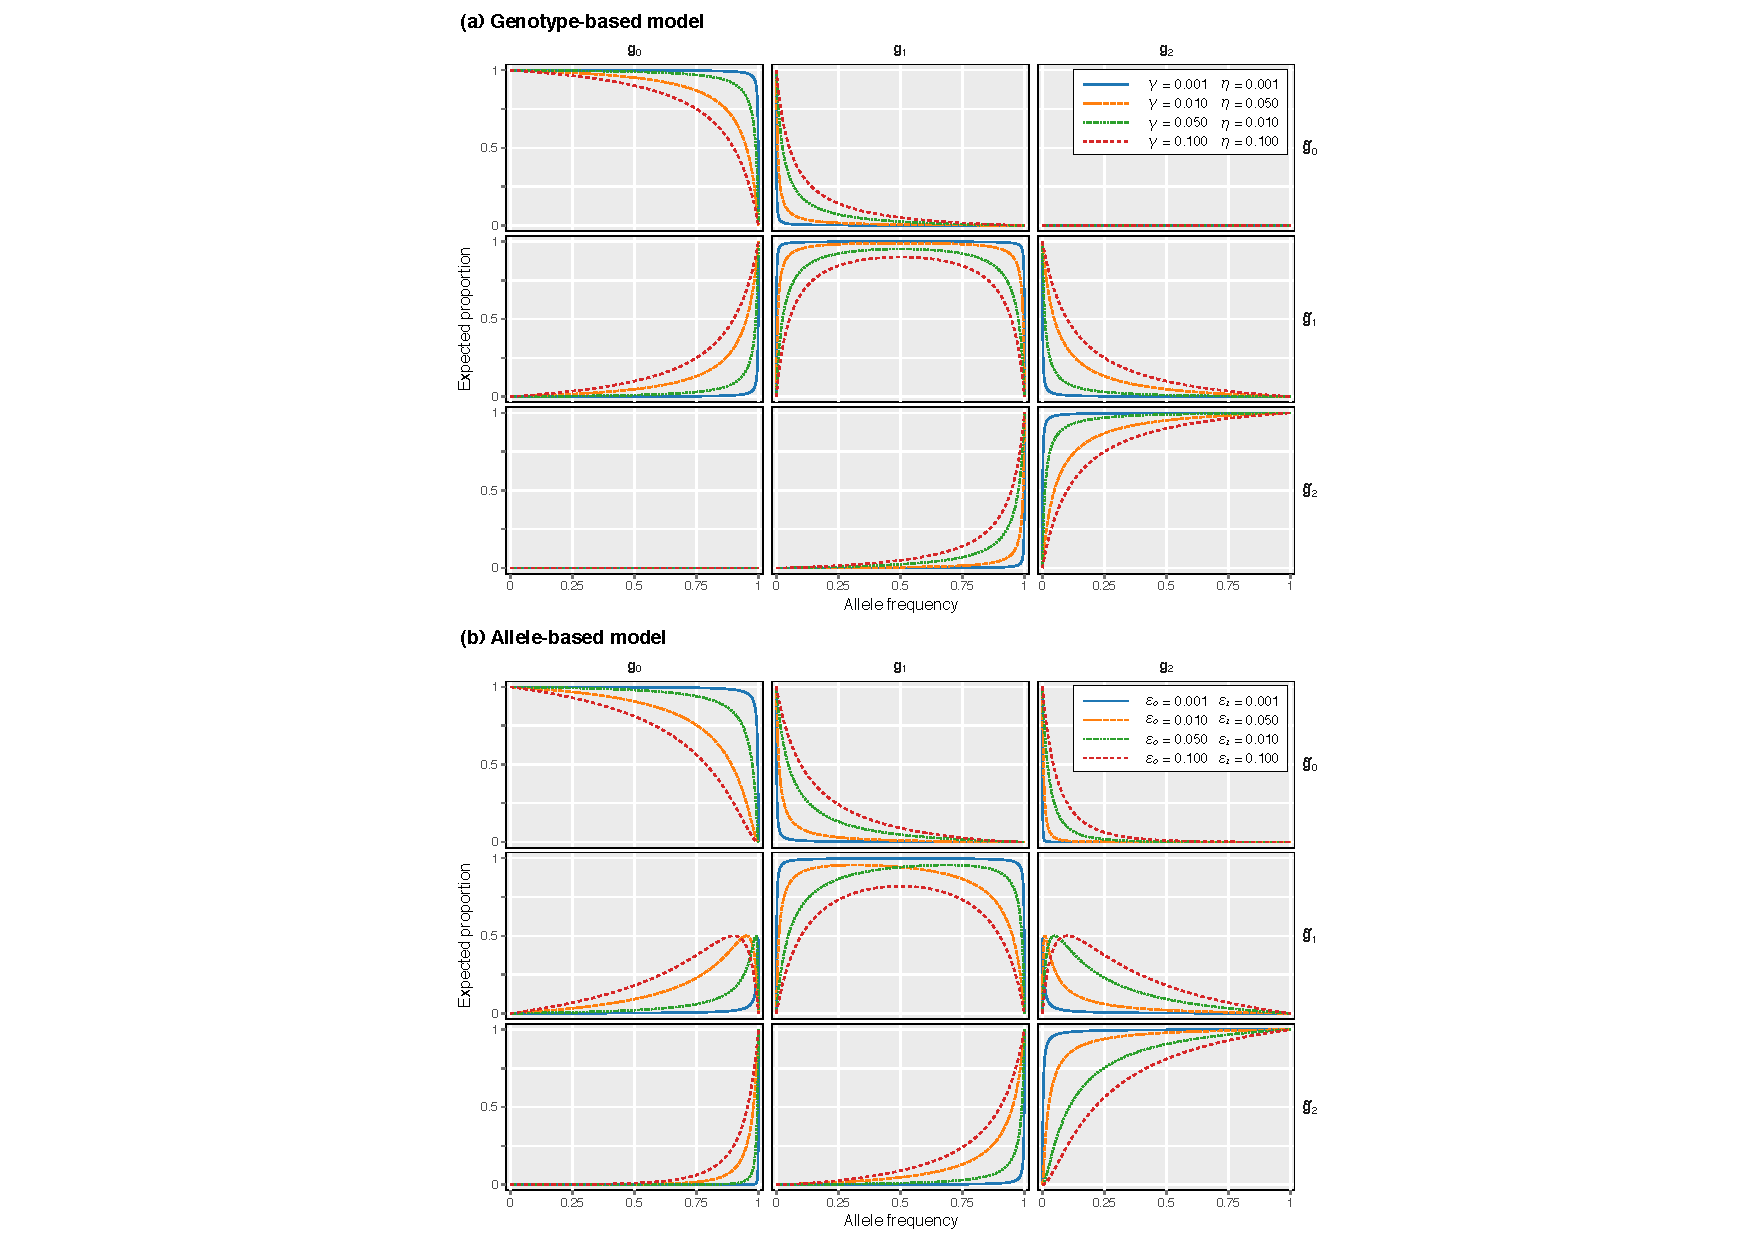
\includegraphics[width=\textwidth]{./img/ch4/error_models}
\Caption{Expected proportions of genotype error for the genotype and allele-based models}
{The graphs show the expected proportions of true genotypes ($g$) that make up an observed genotype ($\tilde{g}$) given the true allele frequency; calculated at different, nominal error rates (see legend).
The error functions provided in \cpref{tab:errormodel} were used as in \cpref{eq:errfrqprob} and results were normalised to sum to 1 per observed genotype (columns).\AdditionLabel}
{fig:error_models}
\end{figure}

%

\Correct{Error} functions for both models are given in \cpref{tab:errormodel}; note that these are arranged as in error matrix $\mathcal{E}$ in \cref{eq:errormatrix}.
\Addition{To illustrate the expectations arising from these models, \cpref{fig:error_models} shows the expected proportion of a true genotype observed as the same or another genotype, at different, nominal error rates, for both the genotype and allele-based models.}
\Addition{It should be noted that the error parameters specified in each model may not apply equally to each variant in genomic data, due to differences arising from technical bias in the sequencing or genotyping process and variations in the accessibility of DNA along the genome (\eg chromatin structure variations near telomeric or centromeric regions).}

In the following section, I estimated genotype \Correct{error rates} in different datasets.
In each, error was computed from the proportions of correctly and incorrectly classified genotypes, such that error parameters were estimated for each model.






%
\section{Generation of platform-specific genotype error profiles}
\label{sec:generrprofiles}
%

Assessment of genotype accuracy requires the existence of an error-free ``gold~standard'' dataset against which data generated on other platforms can be compared; provided that data were obtained on the same biological sample.
In reality, however, the possibility of undetected genotype error cannot be excluded, but it can be reduced, for example, based on pedigree information and the laws of Mendelian inheritance.
In the section below, I describe the dataset which I used as a reference for high-confidence genotype data.
These were compared to several publicly available datasets generated using different genotyping and sequencing technologies, which included individuals also present in the reference dataset.

%
\subsection{High-confidence genome data as benchmark for comparisons}
%

The analysis was based on data from the \gls{ipg},\footnote{Illumina Platinum Genomes: \url{http://www.illumina.com/platinumgenomes/} \accessed{2016}{11}{16}} which comprises a \n{17}-member, \n{3}-generation family of European ancestry; CEPH~pedigree~1463.\footnote{Centre d'Etude du Polymorphisme Humain (CEPH), Utah family pedigree 1463: \url{https://catalog.coriell.org/0/Sections/Collections/NIGMS/CEPHFamiliesDetail.aspx?fam=1463} \accessed{2016}{11}{16}}
This dataset has been generated using recent state-of-the-art sequencing technologies and methods for variant calling, where a total of 5.43~million variants were identified genome-wide \citep{Eberle:2016ki}; this included 4.73~million \glspl{snp}.
Individuals had been sequenced to a depth of 50x on Illumina HiSeq~2000, and variants were called in concordance to several variant calling methods.
Notably, due to the availability of pedigree information, artefacts such as genotype errors had been excluded based on deviations from Mendelian inheritance.
The dataset comprises \n{11} children from \n{2} parents, who themselves are the children of the \n{4} founders of the pedigree; see \cpref{fig:ceph1463}.
Thus, inheritance constraints were most informative for the \n{2} parents, labelled \textsf{NA12877} and \textsf{NA12878} (Coriell~ID), which were additionally sequenced to 200x depth, and for which high-confidence variant calls were made available.

%
%!TEX root = ../../main.tex


\begin{figure}[!htb]
\centering
\vspace{5pt}
\begin{tikzpicture}[-,auto,thick,font=\sffamily\footnotesize,
F/.style={circle,draw,fill=white,ultra thick,minimum size=4mm,outer sep=3pt},
M/.style={rectangle,draw,fill=white,ultra thick,minimum size=4mm,outer sep=3pt},
mate/.style={cross out,draw=black,minimum size=2mm,inner sep=0pt,outer sep=0pt}]

\newcommand{\springoff}[2]{
\draw[-,rounded corners=5pt] (#1.south) |- (#2);
}
\newcommand{\offspring}[2]{
\path (#1) -- (#2.north) coordinate[pos=0.5] (mid);
\draw[-,rounded corners=3pt] (#1) |- (mid) -| (#2.north);
}

\node[M,fill=Ivory2] (a) at (3.25,4) {};
\node[mate]  at (4.00,4) {};
\node[F,fill=Ivory2] (b) at (4.75,4) {};
\node[M,fill=Ivory2] (c) at (6.25,4) {};
\node[mate]  at (7.00,4) {};
\node[F,fill=Ivory2] (d) at (7.75,4) {};

\coordinate (A) at (4,3.5);
\coordinate (B) at (7,3.5);

\node[M,fill=Chocolate3,label={left:NA12877}] (77) at (4,2.5) {};
\node[mate] at (5.5,2.5) {};
\node[F,fill=Chocolate3,label={right:NA12878}] (78) at (7,2.5) {};

\coordinate (P) at (5.5,2);

\node[F,fill=Ivory2] (1) at (1,1) {};
\node[F,fill=Ivory2] (2) at (2,1) {};
\node[F,fill=Ivory2] (3) at (3,1) {};
\node[M,fill=Ivory2] (4) at (4,1) {};
\node[M,fill=Ivory2] (5) at (5,1) {};
\node[M,fill=Ivory2] (6) at (6,1) {};
\node[F,fill=Ivory2] (7) at (7,1) {};
\node[M,fill=Ivory2] (8) at (8,1) {};
\node[F,fill=Ivory2] (9) at (9,1) {};
\node[M,fill=Ivory2] (10) at (10,1) {};
\node[M,fill=Ivory2] (11) at (11,1) {};


\springoff{a}{A}
\springoff{b}{A}
\draw [-] (A) to (77.north);

\springoff{c}{B}
\springoff{d}{B}
\draw [-] (B) to (78.north);

\springoff{77}{P}
\springoff{78}{P}

\offspring{P}{1}
\offspring{P}{2}
\offspring{P}{3}
\offspring{P}{4}
\offspring{P}{5}
\offspring{P}{6}
%\draw [-] (P) to (6.north);
\offspring{P}{7}
\offspring{P}{8}
\offspring{P}{9}
\offspring{P}{10}
\offspring{P}{11}

\end{tikzpicture}
\vspace{5pt}
\Caption{CEPH pedigree 1463}%
{The pedigree of the family sequenced in the \glsentrylong{ipg}.
Genotype data of individuals \textsf{NA12877} and \textsf{NA12878} (indicated) were used as reference against which data obtained on other genotyping or sequencing platforms were compared.
Figure modified from \citet{Eberle:2016ki}, Figure~1.}%
{fig:ceph1463}
\end{figure}

%

Genotype (\gls{snp}) data from \gls{ipg} for individuals \textsf{NA12877} and \textsf{NA12878} were used as reference or \emph{truth} for comparison to concordant data obtained on other platforms.
Although the possibility of genotype error in \gls{ipg} data cannot be excluded, it is assumed that error rates in \textsf{NA12877} and \textsf{NA12878} are sufficiently low to allow proportional estimation of genotype misclassification rates based on observations over thousands of variant sites.
%Likewise, the probability of double-error, if both ``true'' and ``observed'' genotypes are misclassified at single loci, was ignored as it was assumed to be negligibly small.

Due to the imperfection of even high-standard sequencing technologies, not all chromosomal regions are equally accessible, which affects the power to determine variants in the calling process along the length of the sequence.
The confidence of variant calls is derived from the depth of mapped sequence reads and quality scores.
To maintain high levels of confidence in the data, accessibility masks provided by \gls{ipg} were applied such that only sites in high-confidence regions were retained in the analysed datasets.
This retained a sum of \dec{3.407}~million and \dec{3.605}~million \glspl{snp} for \textsf{NA12877} and \textsf{NA12878}, respectively, across chromosomes~1--22.


%
\subsection{Selection and preparation of datasets from different platforms}
%

Because cell lines from CEPH~pedigree~1463 are a well-characterised model system, either \textsf{NA12877} or \textsf{NA12878}, or both, have been assessed in several studies.
For example, CEPH~pedigree~1463 was genotyped in the \glsentrylong{hapmap}, which was one of the first large-scale catalogues of human genetic variation \citep{Thorisson:2005ff,Frazer:2007kha,InternationalHapMapConsortium:2010en}.
Considering a more recent example, the \glsentrylong{1kg} provides data obtained on several platforms, including \gls{wgs} and high-density genotyping technologies \citep{Durbin:2010gj,GenomesProjectConsortium:2012co,Auton:2015gk}.

It must be noted that the process of acquiring data is substantially different for genotyping and sequencing methods.
The established approach for genotyping is to use chip or array-based methods, which are designed to target, or ``type'' specific molecular markers at predetermined regions and require prior knowledge about mapped locations in the genome.
On the other hand, sequencing determines the contiguous nucleotide sequence, either genome-wide or for a region of the genome.
Sequence data are aligned against a reference genome and further processed.
Eventually, variants are ``called'' at nucleotides that differ from the reference at each position along the sequence.
%Both types of data can be represented in \gls{vcf}.

Genotype error profiles were generated for both sequencing and genotyping data, which were taken from available resource data of the \glsentrylong{1kg}.
The following \emph{test} datasets were included:
\begin{itemize}
\item Low-coverage sequencing data from the final release of \glsentrylong{1kg} Phase~\rom{3} (\textbf{\emph{1000G}}), generated on Illumina HiSeq~2000 and HiSeq~2500 platforms (2-4x), and consisting of 78~million \glspl{snp} in total.
\item Genotyping data generated on Illumina HumanOmni2.5 BeadChip (\textbf{\emph{Omni2.5}}) with 2.46~million \glspl{snp}.
%Note that Omni2.5 does not capture variants below \gls{maf} of 2.5\%.
\item Genotyping data generated on Affymetrix Genome-Wide Human SNP Array~6.0 (\textbf{\emph{Affy6.0}}) with 0.91~million \glspl{snp}.
\end{itemize}
To acknowledge differences arising from the variant calling and filtering process in sequencing data, \n{2} \emph{1000G} profiles were created; one that included all variant sites (\textbf{\emph{1000G.A}}), and one containing only sites within high-confidence regions (\textbf{\emph{1000G.B}}).
For the latter, the ``strict'' accessibility mask provided by \glsentrylong{1kg} Phase~\rom{3} was used \citep[see][supplementary information 9.2]{Auton:2015gk}.\footnote{Accessible genome masks in 1000G: \url{http://ftp.1000genomes.ebi.ac.uk/vol1/ftp/release/20130502/supporting/accessible_genome_masks/} \accessed{2016}{11}{27}}
Note that the sample of the final release dataset of \emph{1000G} included \textsf{NA12878}, but not \textsf{NA12877}.
The other \n{2} datasets, \emph{Omni2.5} and \emph{Affy6.0}, which were part of previous releases of the \glsentrylong{1kg}, included both \textsf{NA12877} and \textsf{NA12878}.\footnote{High-density genotyping data, Omni2.5 and Affy6.0 in \gls{1kg}: \url{ftp://ftp.1000genomes.ebi.ac.uk/vol1/ftp/release/20130502/supporting/hd_genotype_chip/} \accessed{2016}{11}{17}}

%
%!TEX root = ../../main.tex


\begin{figure}[!tbp]
\centering
%\hrulefill\\
%\vspace{5pt}
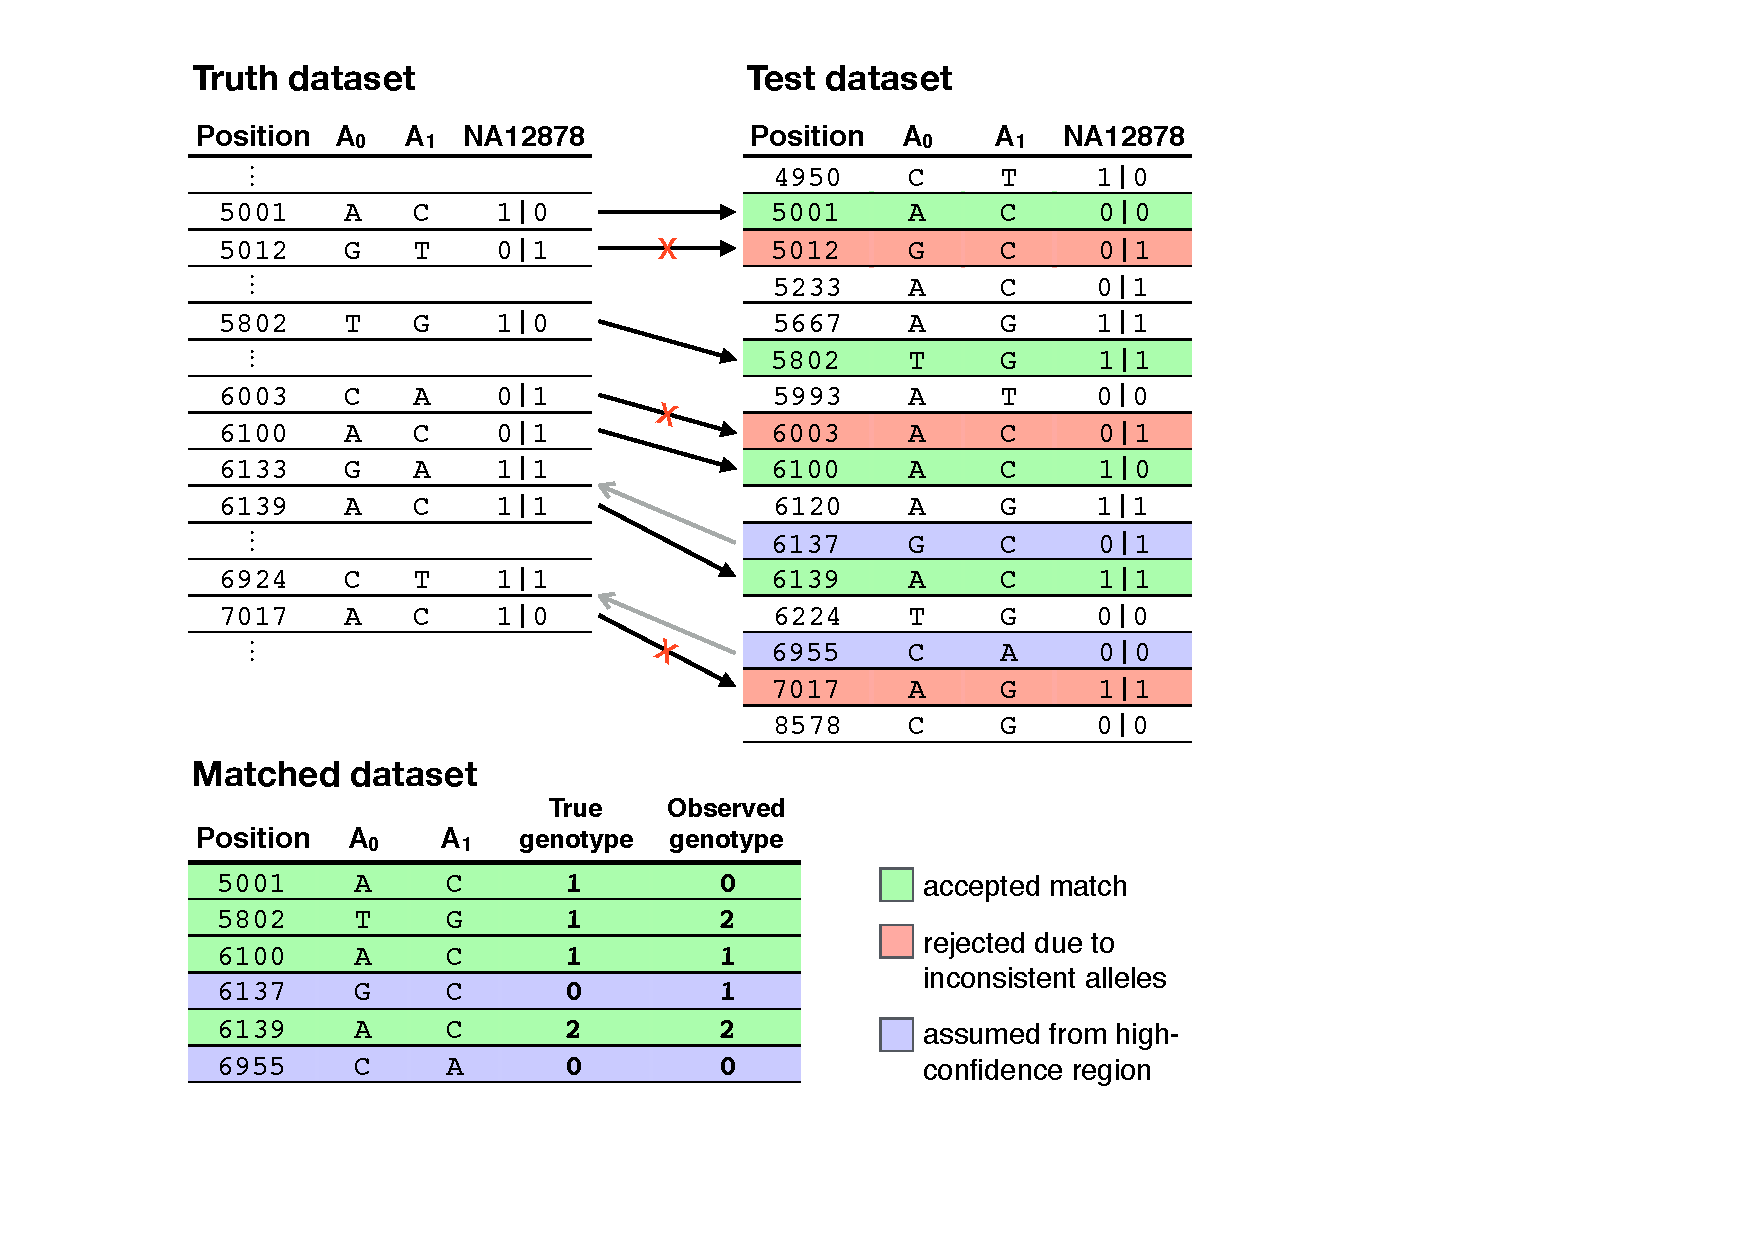
\includegraphics[width=0.75\textwidth]{./img/ch4/info_errormatch}
\Caption{Illustration of the matching process in the generation of error profiles}
{Variant data were reduced to \glspl{snp} and matched per chromosome by variant position and both alleles ($A_0$ and $A_1$) as recorded for either \texttt{NA12877} or \texttt{NA12878}.
Gaps shown in the truth dataset indicate the regions removed after filtering using the accessibility mask provided by \gls{ipg}, such that only high confidence variant calls were retained.
Note that the truth dataset did not contain \glspl{snp} homozygous for the reference allele, but which were assumed from high-confidence regions if present in the test dataset.
This is indicated by left-pointing arrows.}
{fig:info_errormatch}
% \vspace{-5pt}
% \hrulefill%
\end{figure}

%

Misclassification of \gls{snp} genotypes was determined by comparison of each test dataset to the truth dataset, which was done for chromosomes~1--22.
Genotype data were matched by chromosome and variant position (GRCh37/hg19).
As a precaution, sites where reference or alternate nucleotides did not match between test and truth datasets were removed, although only genotypes were compared.

It is important to note that \gls{ipg} data did not contain variants called as being homozygous for the reference allele ($g_0$).
\Addition{\Citet{Eberle:2016ki} identified high-confidence regions in the 13 individual call sets (\textsf{NA12877}, \textsf{NA12878}, and their 11 children) by collating sites that were called as being homozygous for the reference allele and monomorphic in the sample.
Monomorphic variants that were homozygous for the alternate allele were included.}
Therefore, the following assumption was made.
If the position of a variant site in a given test dataset was within high-confidence regions of the \gls{ipg} accessibility mask \Addition{provided by \citet{Eberle:2016ki}}, but not reported in the truth dataset, the true state was assumed to be the $g_0$~type.
This relies on the expectation that the high-confidence intervals comprised data which would have otherwise been reported as a different type.
This matching process is illustrated in \cpref{fig:info_errormatch}.

At each matched site, the population frequency was assigned as recorded in the full sample of the final \glsentrylong{1kg} Phase~\rom{3} dataset, which contained \n{2504} individuals from several continental populations worldwide.
Sites for which no frequency information was available were removed.
%, which was the case for a fraction of sites in \emph{Omni2.5} and \emph{Affy6.0}.
Then, the retained genotypes in the matched datasets were used to measure the rate at which a true genotype ($g_0$, $g_1$, or $g_2$) was observed as the same or another genotype ($\tilde{g}_0$, $\tilde{g}_1$, or $\tilde{g}_2$).
This was done to obtain estimates for \Correct{error rate} parameters $\varepsilon_{ij}$ in matrix $\mathcal{E}$.






%
\subsection{Rate of genotype error in sequencing and genotyping data}
%

% IDEA Clarify the aims: to generate error profile which can be used in subsequent construction of a probabilistic IBD model; here, to evaluate measured error rates and compare to expectations, eg. higher error near centromere

The total number of matched variant sites was \dec{76.859}~million in \emph{1000G.A}, but of which \dec{73.435}~million ($\approx$96\%) were assumed as homozygous reference genotypes.
\Correct{Recall that this assumption applied only to sites found within the high-confidence regions as specified in the \gls{ipg} accessibility mask.}
A lower amount was available in \emph{1000G.B}, where \dec{59.234}~million genotypes were retained, but of which \dec{56.739}~million ($\approx$96\%) were assumed.

This large proportion of sites at which a true $g_0$~genotype was assumed may not come as a surprise, because there is a high chance that a considerable fraction of the variants present in either test dataset may fall within the lengths covered by high-confidence regions.
However, because $g_0$ genotypes were removed in \gls{ipg} data, it is a necessary assumption that those genotypes can be recovered from high-confidence regions.
Otherwise, error could not be determined for $g_0$~genotypes.
Overall, 0.079\% of genotypes were misclassified in \emph{1000G.A}, and 0.025\% in \emph{1000G.B}.
If assumed $g_0$ genotypes are ignored, thus only considering true genotype classes ${j \in \lbrace 1,2 \rbrace}$, overall error was increased; reaching 0.538\% and 0.183\% in \emph{1000G.A} and \emph{1000G.B}, respectively.

Due to the comparatively lower number of available sites in genotyping data (\emph{Omni2.5} and \emph{Affy6.0}), the matched \texttt{NA12877} and \texttt{NA12878} datasets were merged.
Together, the total number of \Correct{matched genotypes} was \Correct{\dec{4.233817}~million} in \emph{Omni2.5} and \Correct{\dec{1.715609}~million} in \emph{Affy6.0}, and where \Correct{\dec{1.361437}~million ($\approx$32\%)} and \Correct{\dec{0.793548}~million ($\approx$46\%)} \Correct{of true genotypes were assumed as being homozygous for the reference allele}, respectively.
The \Correct{proportion} of misclassified genotypes was \Correct{{\SI{0.2557975}{\percent}}} in \emph{Omni2.5}, and \Correct{{\SI{0.139484}{\percent}}} in \emph{Affy6.0}.
Error decreased in both genotyping datasets if $g_0$ was ignored, yielding \Correct{{\SI{0.06786946}{\percent}}} and \Correct{{\SI{0.1056017}{\percent}}} of misclassified genotypes in \emph{Omni2.5} and \emph{Affy6.0}, respectively.

% The discrepancy between inclusion and exclusion of assumed $g_0$ genotypes indicates a bias towards oversaturation with correctly observed genotypes in both \emph{1000G} datasets, such that genotype accuracy may have been artificially inflated.

In the following, the \Correct{error rate} of genotypes was investigated in greater detail, for which matched sites from each true genotype class were considered; first, by exploring the distribution of error along the genome and, second, by true genotype class to obtain empirical \Correct{error rate} estimates, which was then extended to generate frequency-dependent error profiles for each dataset.


%
\subsubsection{Genotype accuracy by chromosomal region}
%

Each chromosome was divided into 1~Mb long chunks to depict the rate of misclassified genotypes over the length of the genome; see \cpref{fig:poserrdens}.
Error densities were calculated by dividing the number of incorrect genotypes by the number of all genomes within each chunk, where chunks with less than \n{100} matched sites were removed.

%
%!TEX root = ../../main.tex


\begin{figure}[tbp]
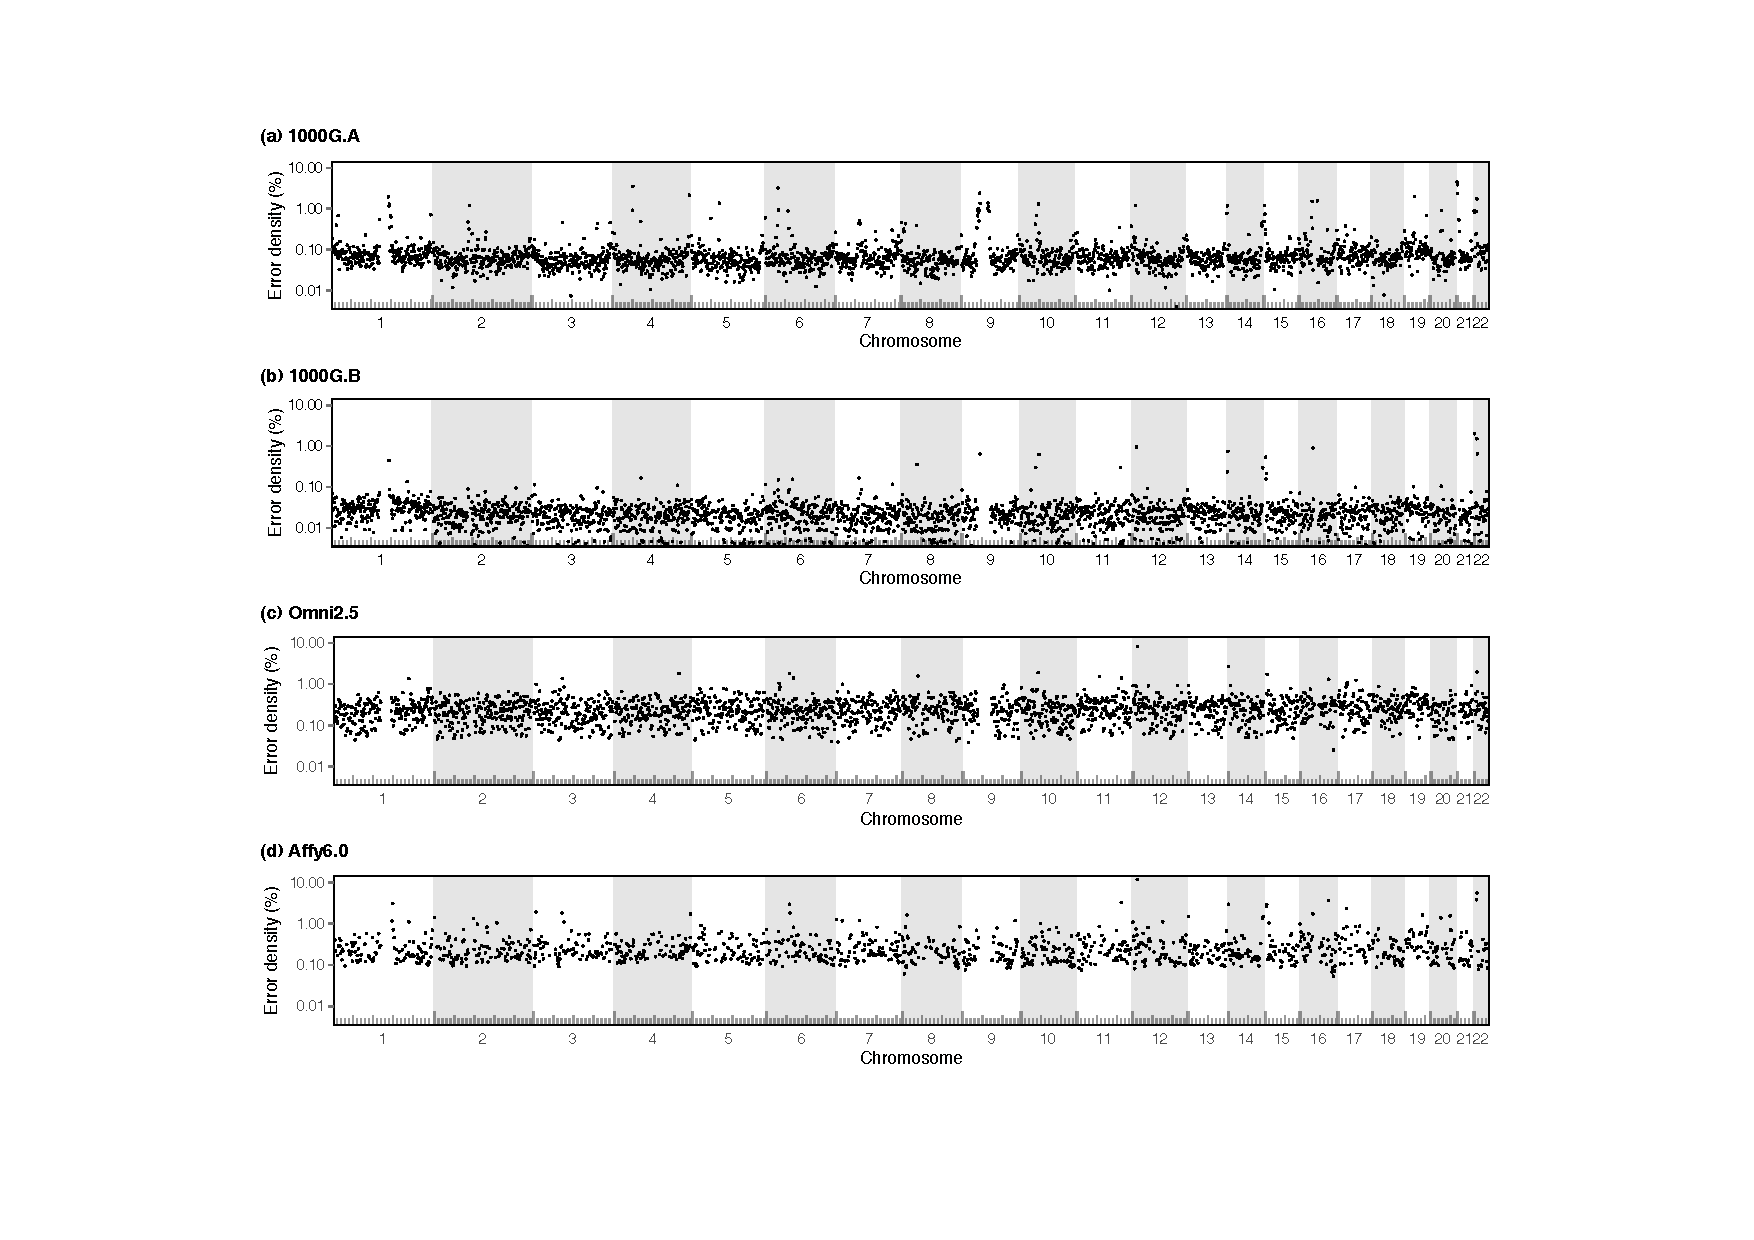
\includegraphics[width=\textwidth]{./img/ch4/poserrdens_new}
\Caption{Positional genotype error density in sequencing and genotyping datasets}%
{The density of misclassified genotypes was calculated along the length of each chromosome, which were divided into equally sized chunks of 1~Mb size.
Error was calculated as the number of misclassified genotypes divided by the total number of genotypes per chunk; percent error shown on log scale.
Chunks with less than 100 genotypes were removed.
The ruler at the bottom edge of each panel shows physical distance per chromosome, where tick marks sit 10~Mb apart.}%
{fig:poserrdens}
% \vspace{-5pt}
% \hrulefill%
\end{figure}

%

The distribution of error in the \emph{1000G.A} dataset was consistently low on average \Correct{({\SI{0.09493559}{\percent}})}, but where error densities increased towards telomere regions and near centromeres, reaching error rates above 1\%.
This is expected, because DNA in the telomeric and centromeric regions is highly repetitive and rich in GC content, which results in difficulties in the amplification process and makes sequence reads difficult to align to the genome.
This pattern was less pronounced in \emph{1000G.B}, as sites outside high-confidence regions were excluded, which resulted in a clear reduction of error along the genome \Correct{on average ({\SI{0.02820162}{\percent}})}.
However, most chromosomes showed locally increased error rates, but where rates above 1\% were rarely observed.
Yet, the persistence of error hotspots indicates that not all low-confidence regions were identified from quality assessment of sequencing data.

In genotyping data, error rates showed less variability along the genome, \eg in the \emph{Omni2.5} dataset, but where error rates averaged \Correct{at {\SI{0.2743292}{\percent}}}, with a few regions of increased error above 5\%.
Although error was low on average in \emph{Affy6.0}, \Correct{averaging at {\SI{0.3078328}{\percent}}}, the likewise lower number of sites resulted in sparse coverage.
However, a few regions showed error rates \Correct{above 5\%, but which were located near the telomeric or centromeric regions.}


%
\subsubsection{Empirical estimation of genotype error rate}
%

Estimates for \Correct{error rate} parameters in $\mathcal{E}$ were derived by considering the proportional relation among observed types per true genotype class.
For each true genotype class $j$, the number of genotypes observed in class $i$ was divided by the total number in class $j$, which gives the empirical value of parameter $\varepsilon_{ij}$; denoted by $\tilde{\varepsilon}_{ij}$.
For an exact formulation, let $n_{ij}$ be the number of observed $\tilde{g}_i$ genotypes whose actual type belongs to the true genotype class $j$.
The empirical value is calculated as
\begin{equation}\label{eq:empexperr}
	\tilde{\varepsilon}_{ij} = \frac{n_{ij}}{N_j} \quad \forall j
\end{equation}
where ${N_j = \sum^{2}_{i=0} n_{ij}}$, \ie the number of all genotypes per true class $j$, such that ${\tilde{\varepsilon}_{0j} + \tilde{\varepsilon}_{1j} + \tilde{\varepsilon}_{2j} = 1 \ \forall \ j}$.
Results for each dataset are presented in \cpref{tab:generrpercent}.

%
% !TEX root = ../../main.tex


\begin{table}[!htb]
\Caption{Measured genotype penetrance in sequencing and genotyping data}
{Genotypes in each true genotype class ($g_0$, $g_1$, and $g_2$) were distinguished by observed genotype class ($\tilde{g}_0$, $\tilde{g}_1$, and $\tilde{g}_2$), to obtain empirical expectations for genotype penetrances $\varepsilon_{ij}$.
Per dataset, proportions sum to 100\% by column.
The total number of genotypes counted per true class are given in the table.\CorrectLabel}
{tab:generrpercent}
\centering
\begin{threeparttable}
\renewcommand{\arraystretch}{1.1}%
\begin{tabular}{lcrrr}
\toprule
 Dataset & Observed genotype & \multicolumn{3}{c}{True genotype} \\ \cmidrule(lr){3-5}
 & & \multicolumn{1}{c}{$g_0$} & \multicolumn{1}{c}{$g_1$} & \multicolumn{1}{c}{$g_2$} \\ \midrule
\textbf{1000G.A}
& $\tilde{g}_0$ & 99.942\% &  0.550\% &  0.033\% \\
& $\tilde{g}_1$ &  0.041\% & 99.281\% &  0.228\% \\
& $\tilde{g}_2$ &  0.017\% &  0.169\% & 99.739\% \\ \cmidrule(lr){2-5}
& \emph{Total} & \num{73435064} & \num{2076115} & \num{1347647} \\ \midrule
\textbf{1000G.B}
& $\tilde{g}_0$ & 99.982\% &  0.193\% &  0.003\% \\
& $\tilde{g}_1$ &  0.013\% & 99.749\% &  0.077\% \\
& $\tilde{g}_2$ &  0.005\% &  0.057\% & 99.920\% \\ \cmidrule(lr){2-5}
& \emph{Total} & \num{56739327} & \num{1515508} & \num{978728} \\ \midrule
\textbf{Omni2.5}
& $\tilde{g}_0$ & 99.655\% &  0.048\% &  0.009\% \\
& $\tilde{g}_1$ &  0.195\% & 99.909\% &  0.021\% \\
& $\tilde{g}_2$ &  0.149\% &  0.043\% & 99.970\% \\ \cmidrule(lr){2-5}
& \emph{Total} & \num{3087037} & \num{854327} & \num{522876} \\ \midrule
\textbf{Affy6.0}
& $\tilde{g}_0$ & 99.831\% &  0.081\% &  0.004\% \\
& $\tilde{g}_1$ &  0.093\% & 99.849\% &  0.040\% \\
& $\tilde{g}_2$ &  0.075\% &  0.070\% & 99.956\% \\ \cmidrule(lr){2-5}
& \emph{Total} &  \num{931857} & \num{463649} & \num{337649} \\ \bottomrule
\end{tabular}


%
%%% Correction in Omni and Affy
%
% \begin{tabular}{lcrrr}
% \toprule
%  Dataset & Observed genotype & \multicolumn{3}{c}{True genotype} \\ \cmidrule(lr){3-5}
%  & & \multicolumn{1}{c}{$g_0$} & \multicolumn{1}{c}{$g_1$} & \multicolumn{1}{c}{$g_2$} \\ \midrule
% \textbf{1000G.A}
% & $\tilde{g}_0$ & 99.942\% &  0.550\% &  0.033\% \\
% & $\tilde{g}_1$ &  0.041\% & 99.281\% &  0.228\% \\
% & $\tilde{g}_2$ &  0.017\% &  0.169\% & 99.739\% \\ \cmidrule(lr){2-5}
% & \emph{Total} & \num{73435064} & \num{2076115} & \num{1347647} \\ \midrule
% \textbf{1000G.B}
% & $\tilde{g}_0$ & 99.982\% &  0.193\% &  0.003\% \\
% & $\tilde{g}_1$ &  0.013\% & 99.749\% &  0.077\% \\
% & $\tilde{g}_2$ &  0.005\% &  0.057\% & 99.920\% \\ \cmidrule(lr){2-5}
% & \emph{Total} & \num{56739327} & \num{1515508} & \num{978728} \\ \midrule
% \textbf{Omni2.5}
% & $\tilde{g}_0$ & 98.349\% &  0.110\% &  0.011\% \\
% & $\tilde{g}_1$ &  0.869\% & 99.838\% &  0.021\% \\
% & $\tilde{g}_2$ &  0.782\% &  0.052\% & 99.968\% \\ \cmidrule(lr){2-5}
% & \emph{Total} & \num{3087037} & \num{854327} & \num{522876} \\ \midrule
% \textbf{Affy6.0}
% & $\tilde{g}_0$ & 99.786\% &  0.081\% &  0.004\% \\
% & $\tilde{g}_1$ &  0.116\% & 99.849\% &  0.040\% \\
% & $\tilde{g}_2$ &  0.098\% &  0.071\% & 99.956\% \\ \cmidrule(lr){2-5}
% & \emph{Total} &  \num{931857} & \num{463649} & \num{337649} \\ \bottomrule
% \end{tabular}

% \begin{tabular}{@{}crrrrrrrr@{}}
% \toprule
% \multicolumn{2}{c}{} & \multicolumn{3}{c}{Confident} & \multicolumn{1}{c}{} & \multicolumn{3}{c}{Strictly confident} \\
% \cmidrule(lr){3-5} \cmidrule(l){7-9}
% \multicolumn{2}{c}{} & \multicolumn{1}{c}{$g_0$} & \multicolumn{1}{c}{$g_1$} & \multicolumn{1}{c}{$g_2$} & \multicolumn{1}{c}{} & \multicolumn{1}{c}{$g_0$} & \multicolumn{1}{c}{$g_1$} & \multicolumn{1}{c}{$g_2$} \\
% \midrule
% \multicolumn{9}{@{}l}{\textbf{1000G}} \\
% $\tilde{g}_0$ &
% & 99.942\% &  0.550\% &  0.033\% &
% & 99.982\% &  0.193\% &  0.003\% \\
% $\tilde{g}_1$ &
% &  0.041\% & 99.281\% &  0.228\% &
% &  0.013\% & 99.749\% &  0.077\% \\
% $\tilde{g}_2$ &
% &  0.017\% &  0.169\% & 99.739\% &
% &  0.005\% &  0.057\% & 99.920\% \\
% \cmidrule(lr){3-5} \cmidrule(l){7-9}
% Total &
% & \num{73435064} & \num{2076115} & \num{1347647} &
% & \num{56739327} & \num{1515508} & \num{978728} \\
% \midrule
% \multicolumn{9}{@{}l}{\textbf{Omni2.5}} \\
% $\tilde{g}_0$ &
% & 98.349\% &  0.110\% &  0.011\% &
% & 99.102\% &  0.053\% &  0.006\% \\
% $\tilde{g}_1$ &
% &  0.869\% & 99.838\% &  0.021\% &
% &  0.486\% & 99.917\% &  0.016\% \\
% $\tilde{g}_2$ &
% &  0.782\% &  0.052\% & 99.968\% &
% &  0.412\% &  0.030\% & 99.977\% \\
% \cmidrule(lr){3-5} \cmidrule(l){7-9}
% Total &
% & \num{3087037} & \num{854327} & \num{522876} &
% & \num{2829681} & \num{797011} & \num{484441} \\
% \midrule
% \multicolumn{9}{@{}l}{\textbf{Affy6.0}} \\
% $\tilde{g}_0$ &
% & 99.786\% &  0.081\% &  0.004\% &
% & 99.859\% &  0.076\% &  0.002\% \\
% $\tilde{g}_1$ &
% &  0.116\% & 99.849\% &  0.040\% &
% &  0.079\% & 99.858\% &  0.037\% \\
% $\tilde{g}_2$ &
% &  0.098\% &  0.071\% & 99.956\% &
% &  0.062\% &  0.065\% & 99.961\% \\
% \cmidrule(lr){3-5} \cmidrule(l){7-9}
% Total &
% & \num{931857} & \num{463649} & \num{337649} &
% & \num{892628} & \num{441291} & \num{317926} \\
% \bottomrule
% \end{tabular}

\begin{tablenotes}[para]\footnotesize
Note that true genotypes homozygous for the reference allele, $g_0$, were not present in \gls{ipg} and assumed from high-confidence regions if present in a given test dataset.
\end{tablenotes}
\end{threeparttable}
\end{table}

%

In all \n{4} datasets, values for $\tilde{\varepsilon}_{ij}$ were highest when genotypes were classified correctly; \ie ${i = j}$, the main diagonal in $\mathcal{E}$.
Notably, $\tilde{\varepsilon}_{00}$ was highest in all sequencing datasets, whereas $\tilde{\varepsilon}_{22}$ was highest in genotyping datasets.
%This again suggests that in the sequencing datasets more $g_0$ genotypes were correctly observed than expected.
In each dataset, true homozygous genotypes were more likely to be misclassified as heterozygotes than as the opposite homozygote, but the probability to observe opposite homozygotes was non-zero throughout.
Misclassification of true heterozygous genotypes showed a preference towards genotypes that are homozygous for the reference allele; except in \emph{Affy6.0} where misclassification rates were nearly equal for $\tilde{g}_0$ and $\tilde{g}_2$.
As formulated in \ctref{eq:errfrqprob}, the observed genotype frequency is a function of the true allele frequency and \Correct{error rates} of genotypes.
Hence, the frequency-dependent distribution of empirical \Correct{error rate} was assessed; see section below.


%
\subsubsection{Frequency-dependent genotype error distribution}
%

For each true genotype class, sites were pooled by their assigned population allele frequencies
into \n{200} frequency bins of equal scope on linear scale; \ie bins were separated in steps of 0.5\%.
Using \ctref{eq:empexperr}, the proportions of observed genotypes were calculated in each bin, to obtain \Correct{error rate} expectations across the frequency spectrum.
Additionally, because it can be expected that $N_j$ becomes small at lower genotype frequencies, bins where the number of genotypes dropped below a nominal threshold were marked to indicate less support for estimated \Correct{error rates}.
\N{3} nominal levels of support were distinguished;
\begin{align*}
	\textit{Low support}     & \quad\text{if}\quad {N_j < 100}\ , \\
	\textit{Reduced support} & \quad\text{if}\quad {100 \leq N_j < 1000}\ , \\
	\textit{High support}    & \quad\text{if}\quad {N_j \geq 1000}\ .
\end{align*}

%
%!TEX root = ../../main.tex


\begin{figure}[!htbp]
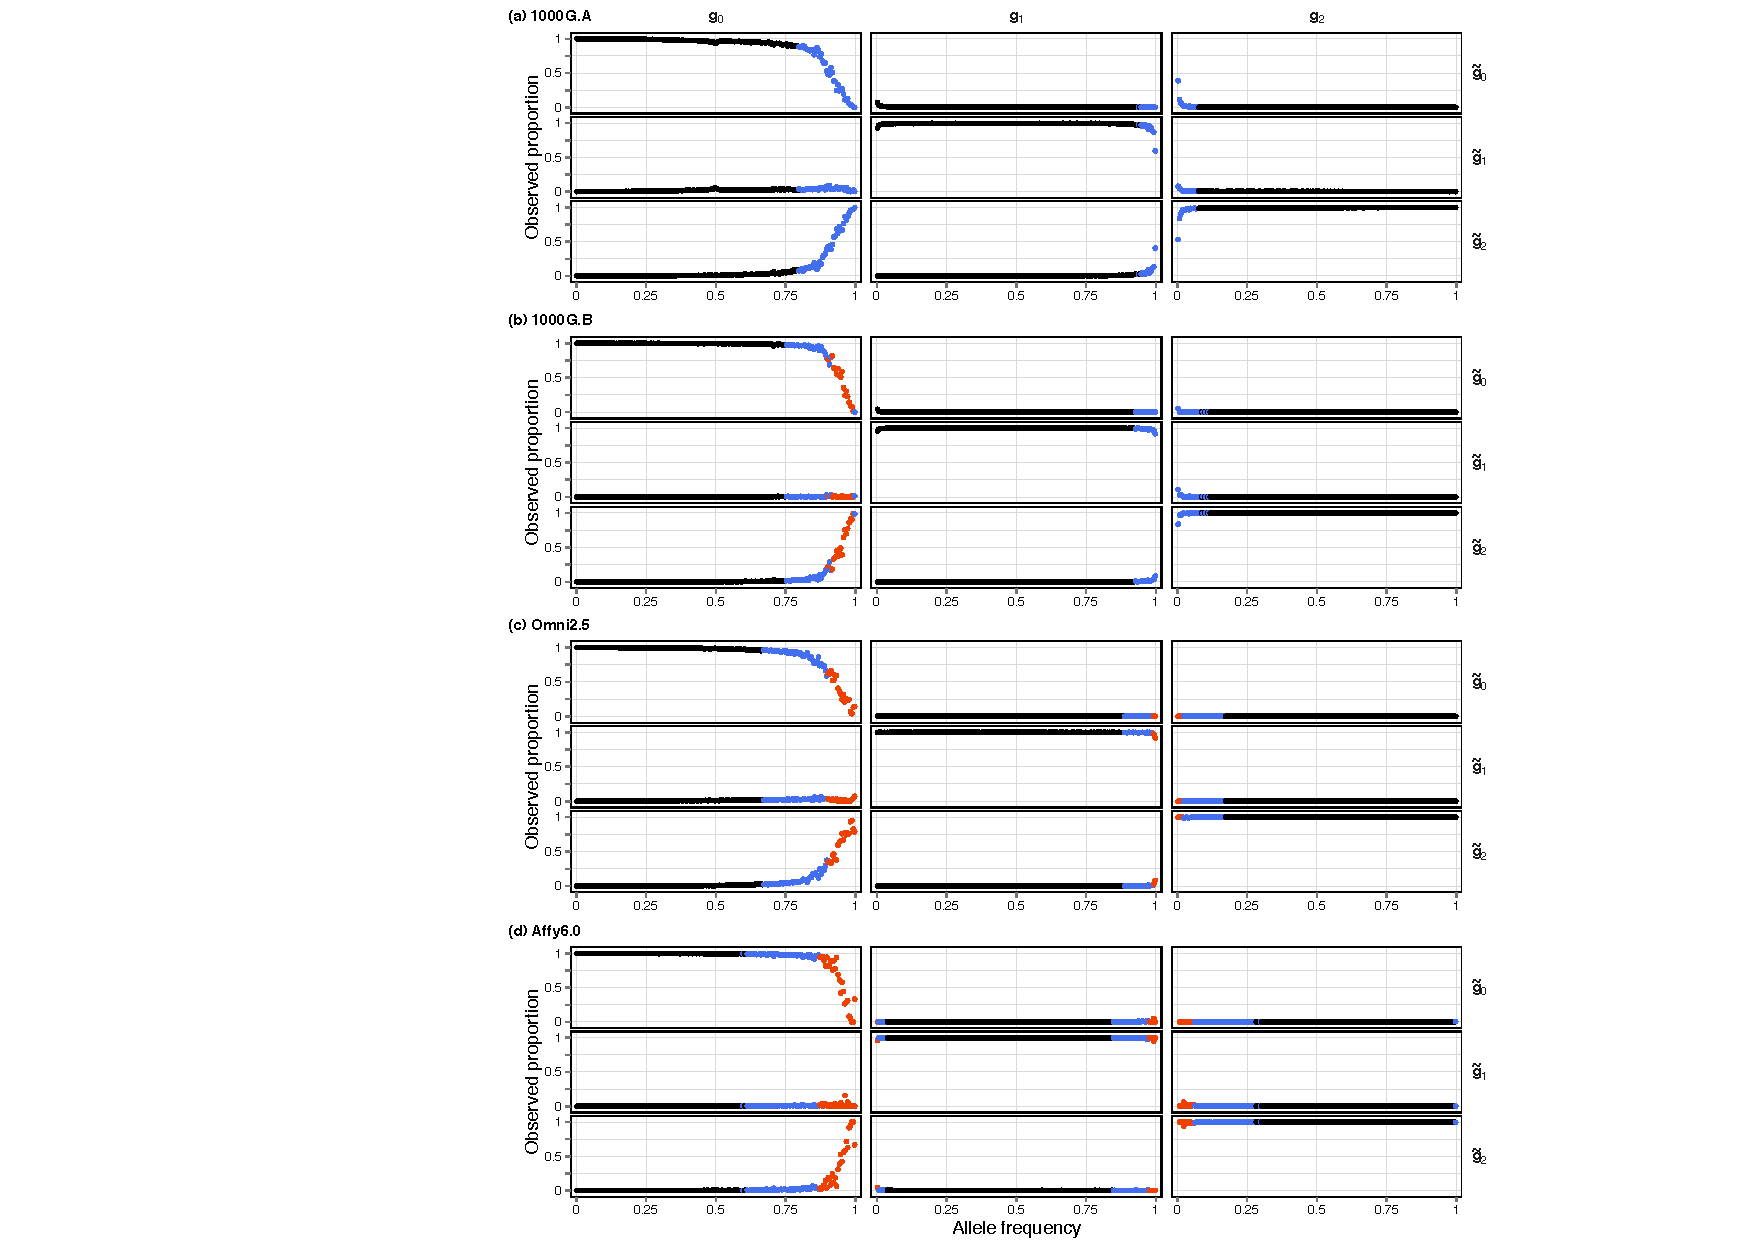
\includegraphics[width=\textwidth]{./img/ch4/generrprop}
\Caption{Empirical error rates in sequencing and genotyping data}%
{For each true genotype class (columns), the fraction of $g_j$ observed as $\tilde{g}_i$ (rows) was calculated per allele frequency bin, to estimate the frequency-dependent distribution of genotype penetrance $\varepsilon_{ij}$.
The set of matched genotypes per true genotype class was divided into \n{200} bins along the allele frequency spectrum.
Allele frequency was assigned to each matched site in a given test dataset, taking the population frequency as recorded in the full sample of the \glsentrylong{1kg} phase~\rom{3} dataset (\n{2504} individuals).
Colours indicate the number of genotypes per bin, $N_{j}$, distinguished at nominal thresholds ${N_j < 100}$ (\emph{red}), ${100 \leq N_j < 1000}$ (\emph{blue}), and ${N_j \geq 1000}$ (\emph{black}).
Note that true genotypes homozygous for the reference allele, $g_0$, were not present in \gls{ipg} and assumed from high-confidence regions if present in a given test dataset.}%
{fig:generrprop}
\end{figure}
\label{sec:emp_gen_err_prop}
%

For each dataset, the resulting \Correct{error rate} distributions are shown in \cpref{fig:generrprop}.
The proportion of $g_0$ observed as $\tilde{g}_1$ was low throughout.
This effect was seen in all \n{4} datasets, regardless of level of support, which was low for bins above 80\% frequency in all datasets (except \emph{1000G.A} with reduced support).
The most striking observation is the loss of accuracy for true $g_0$ genotypes at higher allele frequencies.
For example in \emph{1000G.A}, the proportion of $g_0$ genotypes that were misclassified as $\tilde{g}_2$ increased substantially towards 100\% alternate allele frequency.

\Correct{However, this pattern should be interpreted with caution, due to the imperfect matching process between data generated on different platforms and, in particular, because the set of true homozygous reference genotypes had to be assumed from high-confidence regions in \gls{ipg} data.
For example, it is expected that $g_0$ genotypes are rarely observed at higher allele frequencies in a sample.
Given that several hundred $g_0$ genotypes were seen at relatively high population frequencies makes it likely that a large proportion of $g_2$ genotypes were falsely assumed as $g_0$;
\eg due to missed or filtered variant calls.}

\Correct{Another} explanation for this observation may be seen in somatic mutations in the sampled biological material.
Data for both \textsf{NA12877} and \textsf{NA12878} were generated from lymphoblastoid cell lines created from sampled B-Lymphocyte cells.
For example, it has been shown that induced pluripotent stem cells may accumulate genetic modifications \citep{Gore:2011id}.
Although CEPH cell lines are often used as a renewable resource of DNA, the possibility that cell lines undergo further genetic modifications may not be excluded.
However, here, because the \gls{ipg} protocol would have excluded sites that showed cell line artefacts, it is assumed that the genotypes had to be consistent with Mendelian laws.
Regardless, note that salient patterns of genotype error were most apparent for the assumed subset of the data; \ie at sites not actually contained in the set of reported genotypes.
It is therefore possible that not all unobserved homozygous reference genotypes can be assumed from high-confidence regions when sites are only observed in other data.


In the opposite homozygote class, $g_2$, observed distributions were mirrored, such that the loss of accuracy occurred at lower frequencies; yet, the proportion of misclassified genotypes was markedly lower.
Under the allele-based error model, this asymmetry suggests that the probability of the alternate allele to appear as the reference allele was higher than in reverse direction, such that ${\epsilon_0 < \epsilon_1}$; see \cpref{tab:errormodel}.


The estimated error distributions were used to reproduce empirical error rates in simulated data.
This was done to assess the effect of genotype misclassification on IBD detection, using the method proposed in Chapter~3; \ie targeted IBD detection done thoroughly, or \texttt{tidy}.
For comparison, an alternate IBD detection method was applied to the same data (\texttt{Refined\,IBD} in \texttt{Beagle\,4.1}; \citealt{Browning:2013eh}).







%
\section{Impact of genotype error on IBD detection}
\label{sec:impact_error_data}
%

One of the genotype error profiles constructed in the previous section was used to induce realistic error patterns in simulated data.
Among the \n{4} test datasets, both sequencing datasets were recorded with higher levels of support.
Although \emph{1000G.B} showed overall lower levels of genotype error, \emph{1000G.A} can be seen as being more representative for data obtained in recent large-scale studies; hence, the integration of error was conducted according to the frequency-dependent \Correct{error rate} distribution in the \emph{1000G.A} profile.
The process of error integration in simulated data is described below.


%
\subsection{Integration of empirical error distributions in simulated data}\label{sec:create_error_data}
%

The dataset simulated in Chapter~3 was re-used for integration of genotype error, so as to enable a direct comparison to previously obtained results after applying the same methodology for IBD detection; see \ctref{sec:msprime} for a description of the simulation process.
Briefly, data were simulated using \texttt{msprime\,0.4.0} \citep{Kelleher:2016fn}, with a sample size of ${N=\num{2500}}$ individuals (\ie \n{5000} haplotypes), resulting in \dec{0.672847}~million variant sites over a length of \SI{62.949301}{\mega\basepair} (\SI{108.26675653}{\centi\morgan}).
Diploid individuals wee formed by pairing haplotypes.
From those, data were converted into genotypes, which were then phased, such that \n{3} datasets were generated (true haplotypes, phased haplotypes, and genotype data).
The same process was followed here; however, genotype error was evoked on haplotype level before haplotype sequences were combined to form genotypes.
By doing so, identically distributed proportions of error were present in both the haplotype and genotype datasets, after conversion of the former into the latter, as well as subsequent phasing.

Haplotypes were randomly assigned into fixed pairs which would later form the genotypes of individuals.
Error was included by randomly replacing haplotype pairs dependent on the empirically determined misclassification rates per true genotype class~$j$.
This was done by selecting each variant site in turn and indexing each haplotype pair that would form genotype~$g_j$ before error.
The index ensured that pairs would be drawn without replacement.
Then, for each class~$j$, indexed pairs were randomly drawn and assigned to each of the \n{3} observed genotype classes, in proportions equal to empirical \Correct{error rates}, as determined for the given allele frequency of the currently selected site.
Haplotype pairs were ``mutated'' according to their assigned class, such that they would form $\tilde{g}_i$ after error.

These haplotype data were then converted into a corresponding genotype dataset, which was then phased using \texttt{SHAPEIT\,2} \citep{Delaneau:2008dk,Delaneau:2013hi}; see description in \cpref{sec:ibd_analysis}.
The \n{3} resulting datasets resembled the original datasets used in the evaluation of IBD inference presented in Chapter~3 (\ctref{sec:ibd_results}), which therefore facilitated assessment in relation to the simulated genealogy and the underlying IBD structure of the sample, as well as a direct comparison to the results generated before error was included.

% Note that, here, frequency-dependent error distributions per genotype class were generated from the \emph{1000G.A} profile by pooling and averaging matched variant sites into \n{200} allele frequency bins.
% This was done to reduce the variance in estimated distributions.
% At each site in the data, penetrance rates were calculated through linear interpolation from averaged values and then normalised such that their sum was equal to~1 per site-frequency.

\Addition{Recall that, for example, the empirically determined proportions of the true $g_0$ class per observed $\tilde{g}_2$ were likely to be inflated at higher allele frequencies; as discussed in \cpref{sec:emp_gen_err_prop}.
Errors reproduced in the simulated dataset may therefore be higher than actually present in the \gls{1kg} dataset.
% For example, the original simulation dataset contained no monomorphic sites, but {\Percent{1.967461}} of all sites were monomorphic after the integration of error.
A more detailed account of the characteristics and consequences of the integration of error in the simulated dataset is given in \cpref{sec:ibd_results_err}.}


%
\subsubsection{Accuracy analysis}
%

The following briefly describes the analyses performed.
\N{2} IBD detection methods were applied to available data; the \texttt{tidy} method as proposed in Chapter~3 and the \texttt{Refined\,IBD} algorithm in \texttt{Beagle\,4.1} \citep{Browning:2013eh}.
Recall that the \texttt{tidy} method is based on inference of recombination events in pairs of individuals to detect breakpoints distal to a given target site, which is enabled by the \gls{fgt}, which requires haplotype data, and the \gls{dgt}, which requires genotype data; see \cpref{sec:tidy}.
Accuracy was measured in terms of the physical distance between breakpoints and focal target position at which IBD segments were identified; calculated using the squared Pearson correlation coefficient, $r^2$, and the \gls{rmsle} as defined in \cpref{eq:rmsle}.
Data were analysed in \n{3} approaches:
\begin{approach_}
\item\label{A4:fgt_h} the \gls{fgt} on the simulated haplotypes and
\item\label{A4:fgt_p} on phased haplotypes, and
\item\label{A4:dgt} the \gls{dgt} on genotype data.
\end{approach_}
Note that the \texttt{Refined\,IBD} algorithm can only be used with haplotype data and was therefore evaluated in \ref{A4:fgt_h} and \ref{A4:fgt_p}.
Again, \fk{} was used to denote the frequency of shared alleles, where $k$ is the allele count in the sample.



%
\subsection{Results}
\label{sec:ibd_results_err}
%

In presence of genotype error, the misclassification of alleles observed to be shared among individuals may pose a problem to the identification of haplotype sharing by descent, in particular for variants that are low in frequency or rare, see \cpref{fig:fk_error}; recall that the \texttt{tidy} method utilises rare allele sharing to identify regions of recent relatedness.
\cref{fig:fk_error}{a} indicates the rate at which genotype data appear at a frequency different to their true frequency due to genotype error; shown for variants below 5\% allele frequency.
The figure shows the change between true and observed allele count, depicted as the difference of the observed minus the true count.
For example, \SI{68.22558}{\percent} of \fk{2}~variants remained at the same frequency, but this fraction decreased for alleles found at higher frequencies, \eg \SI{51.13983}{\percent} for \fk{10} and \SI{28.77095}{\percent} for \fk{50}~variants.

%
% !TEX root = ../../main.tex


\begin{figure}[!htb]
{\footnotesize\texthv{\textbf{(a)}  Misclassification rate}} \\
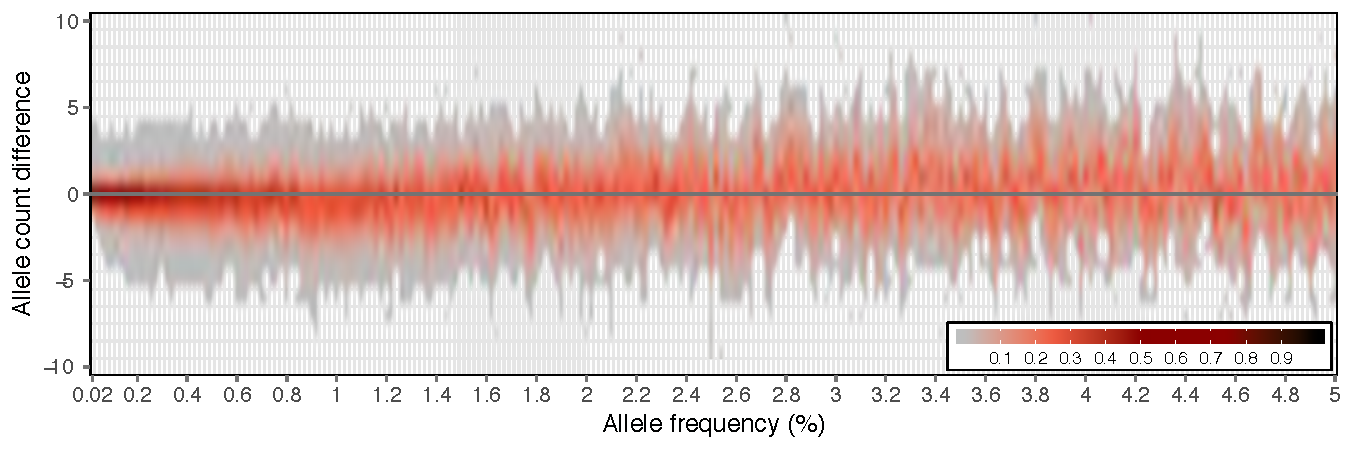
\includegraphics[width=\textwidth]{./img/ch4/fk_error_A_new}
{\footnotesize\texthv{\textbf{(b)}  False positive and false negative rates}} \\
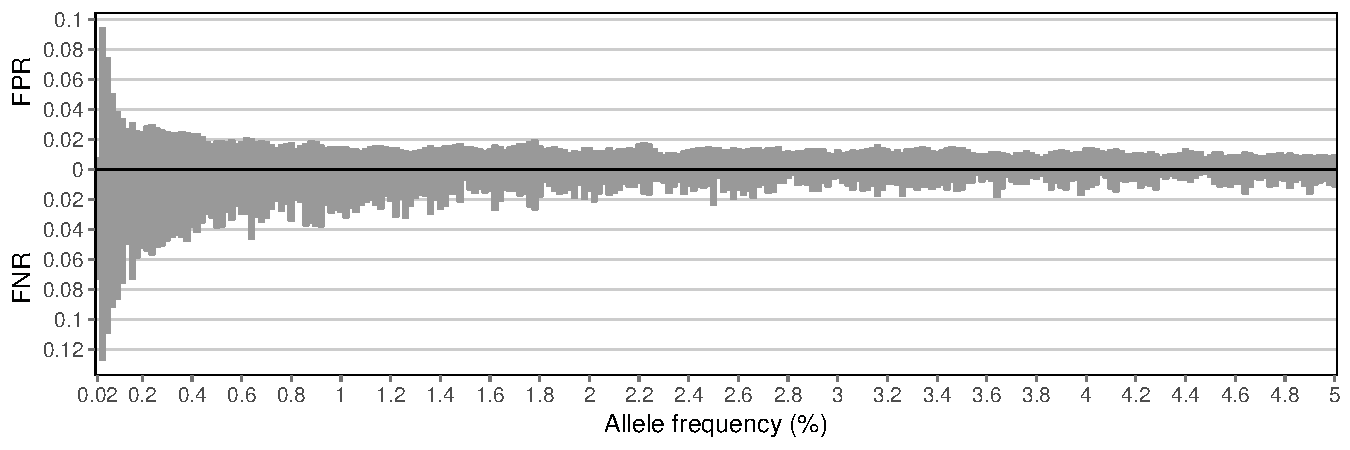
\includegraphics[width=\textwidth]{./img/ch4/fk_error_B}
\Caption{Misclassification of target sites in presence of genotype error}
{Simulated data were modified such that realistic distributions of genotype error were induced.
Panel~\textbf{{(a)}} indicates the rate at which alleles were observed at different frequencies after the inclusion of error.
The proportion of misclassification is indicated by colour intensity.
Panel~\textbf{{(b)}} distinguishes alleles that were falsely observed (false positive) as well as alleles that were missed after the inclusion of error (false negatives).}
{fig:fk_error}
\end{figure}

%

For IBD detection using rare variants as target sites, this may not pose a problem if identified individuals indeed share a given allele.
This is further explored in \cref{fig:fk_error}{b}, where the \gls{fpr} indicates the proportion of alleles that were falsely identified due to $g_0$ or $g_2$ genotypes being observed as $\tilde{g}_1$.
Conversely, the \gls{fnr} indicates the proportion of shared alleles that were missed due to $g_1$ being observed as $\tilde{g}_0$ or $\tilde{g}_2$.
The risk for both types of error was greatest for \fk{2}~variants, here observed at ${\operatorname{FPR}=\dec{0.09356644}}$ and ${\operatorname{FNR}=\dec{0.126583}}$.
On average, \gls{fnr}  (\dec{0.009469898}; ${\pm \dec{0.665030e-3}~\text{SE}}$) was higher than \gls{fpr} (\dec{0.007181344} ; ${\pm \dec{0.403969e-3}~\text{SE}}$), indicating that more shared alleles were missed than falsely observed.



%
\subsubsection{IBD detection using \emph{tidy}}
%

The set of target sites included all \fk{} variants found at ${k \in \lbrace 2, \ldots, 25 \rbrace}$ (\ie alleles shared at frequency ${\leq 0.5\%}$).
In total, \dec{0.296748}~million \glspl{snp} were available in this frequency range, which represented \SI{0.93605}{\percent} of the targets previously identified before the inclusion of error.
Note that sites were only considered if matched to the set of true IBD segments (as previously determined from simulation records).
Hence, false positives were not considered in this analysis.
The number of pairs sharing the focal alleles at available target sites was \dec{10.362361}~million; \ie the total number of IBD segments detected in each approach.

Duplicate segments were removed to retain unique segments after sorting segments by \fk{}, such that segments were associated with the presumably youngest shared allele within the detected breakpoint interval.
Recall that the same IBD interval may be inferred from multiple focal alleles, as these are assumed to sit on the same shared haplotype.
The proportion of uniquely identified segments was \SI{48.03503}{\percent} in \cref{A4:fgt_h},
\SI{48.55437}{\percent} in \cref{A4:fgt_p}, and \SI{41.09449}{\percent} in \cref{A4:dgt}, whereas
\SI{27.40312}{\percent} were unique in the set of true IBD segments.
These sets were then intersected to measure accuracy on the same set of unique IBD segments, which resulted in \dec{2.824385}~million (\SI{27.25619}{\percent}) per approach.

%
% !TEX root = ../../main.tex


\begin{figure}[p]
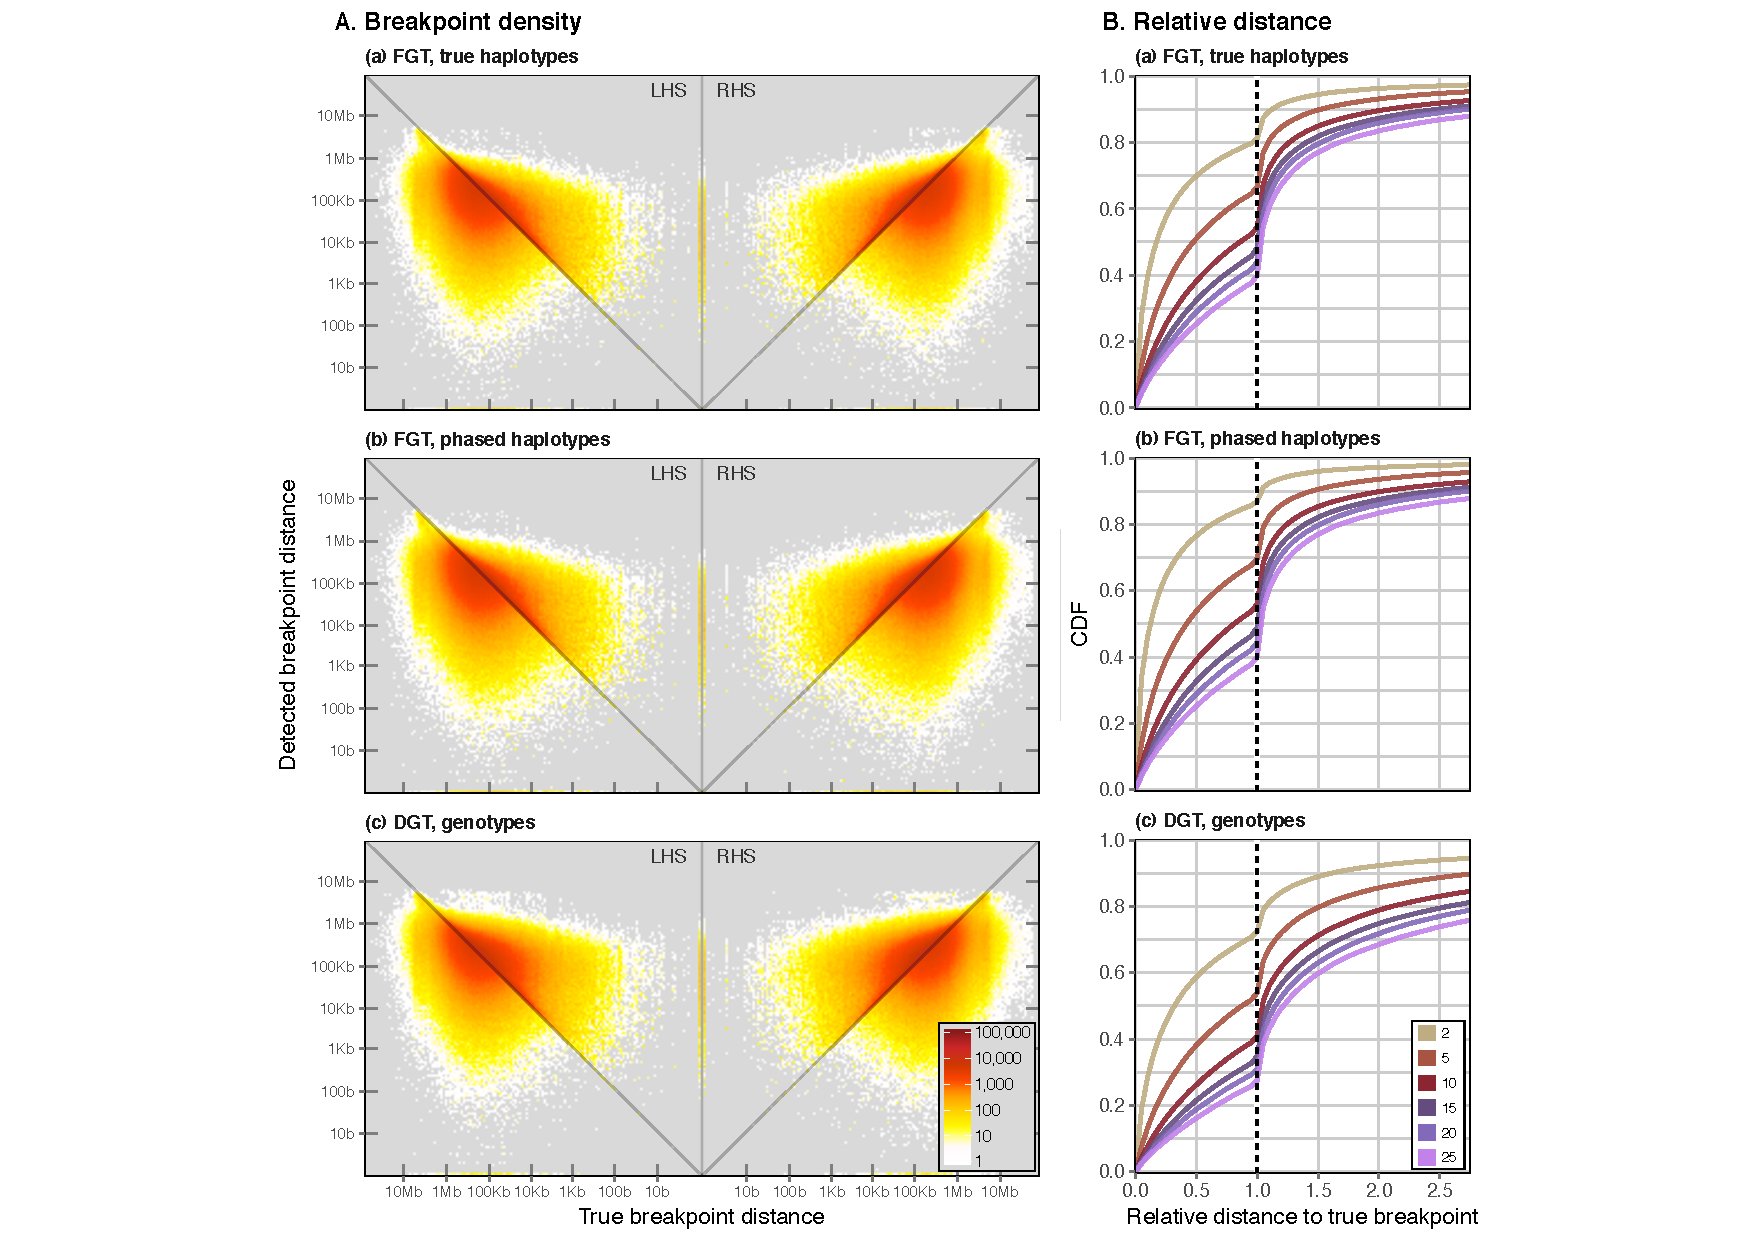
\includegraphics[width=\textwidth]{./img/ch4/break_naive_err}
\Caption{Accuracy of IBD detection using \emph{tidy} after inclusion of genotype error}
{Simulated data after the inclusion of error was analysed using the \gls{fgt} on true haplotypes (a), phased haplotypes (b), and the \gls{dgt} on genotype data (c).
Panel~\textbf{(A)} shows the density of true and detected breakpoints in terms of the physical distance between each detected breakpoint and the corresponding focal site; shown separately for breakpoints detected on the left (LHS) and right-hand side (RHS) of a focal position.
The number of detected and true breakpoints is indicated by colour intensity.
Panel~\textbf{(B)} shows the physical length in terms of the relative distance between a focal site and the detected breakpoint, $\hat{d}$, normalised by the distance to the true breakpoint, $d$; \ie relative distance was calculated as $\rfrac{\hat{d}}{d}$, such that $<1$ indicates underestimation and and $>1$ overestimation of detected breakpoint distance.
This is shown as the cumulative density per \fk{}~variant, for ${k \in \{2, 5, 10, 15, 20, 25\}}$.}
{fig:naive_break_err}
\end{figure}

%

The proportion of breakpoints that were overestimated (in terms of the true distance between target position and actual recombination breakpoint) was
\SI{50.68358}{\percent}, \SI{49.69084}{\percent}, and \SI{63.86433}{\percent} in \ref{A4:fgt_h}, \ref{A4:fgt_p}, and \ref{A4:dgt}, respectively.
Recall that before error was included, the vast majority of breakpoints (${>95\%}$) was overestimated in each approach.
When the \gls{fgt} was used, \SI{49.22148}{\percent} of breakpoints were underestimated and \SI{0.094941}{\percent} coincided with true breakpoints in \cref{A4:fgt_h}, which was similar in \cref{A4:fgt_p} where \SI{50.21720}{\percent} and \SI{0.091966}{\percent} of breakpoints were underestimated and exact, respectively.
When the \gls{dgt} was used, \SI{36.07447}{\percent} of breakpoints were underestimated, but also only \SI{0.061199}{\percent} were exact.

Overall accuracy was low in all approaches; $r^2$ was \dec{0.069374}, \dec{0.072411}, and \dec{0.088683} in \ref{A4:fgt_h}, \ref{A4:fgt_p}, and \ref{A4:dgt}, respectively, which was also reflected in corresponding high error scores (\gls{rmsle}), which were \dec{0.713821}, \dec{0.721678}, \dec{0.693851}, respectively.
For comparison, accuracy measured on the same set of segments, but without genotype error, was ${r^2 > 0.85}$ and \gls{rmsle}~${< 0.55}$ for each approach.
When seen per \fk{}~category, all \n{3} approaches consistently showed low correlation with true segment breakpoints (${r^2 < 0.2}$) and a high magnitude of error (${\rmsle > 0.6}$); see \ctref{tab:stat_hmm_accuracy}, which is shown for comparison to results obtained using the \gls{hmm}-based approach developed in the second part of this chapter.

To determine the lengths of IBD segments in each approach, boundary cases were removed to ensure that breakpoints were detected on both sides of each segment; \SI{0.6221885}{\percent}, \SI{0.6211972}{\percent}, and \SI{0.9235285}{\percent} were removed in \ref{A4:fgt_h}, \ref{A4:fgt_p}, and \ref{A4:dgt}, respectively, but which was noticeably lower compared to boundary cases removed in the set of true IBD segments (\SI{1.359482}{\percent}).
Again, sets were intersected, retaining \dec{2.781729}~million (\SI{98.48972}{\percent}) common segments across approaches.

%
% !TEX root = ../../main.tex


\begin{figure}[!htb]
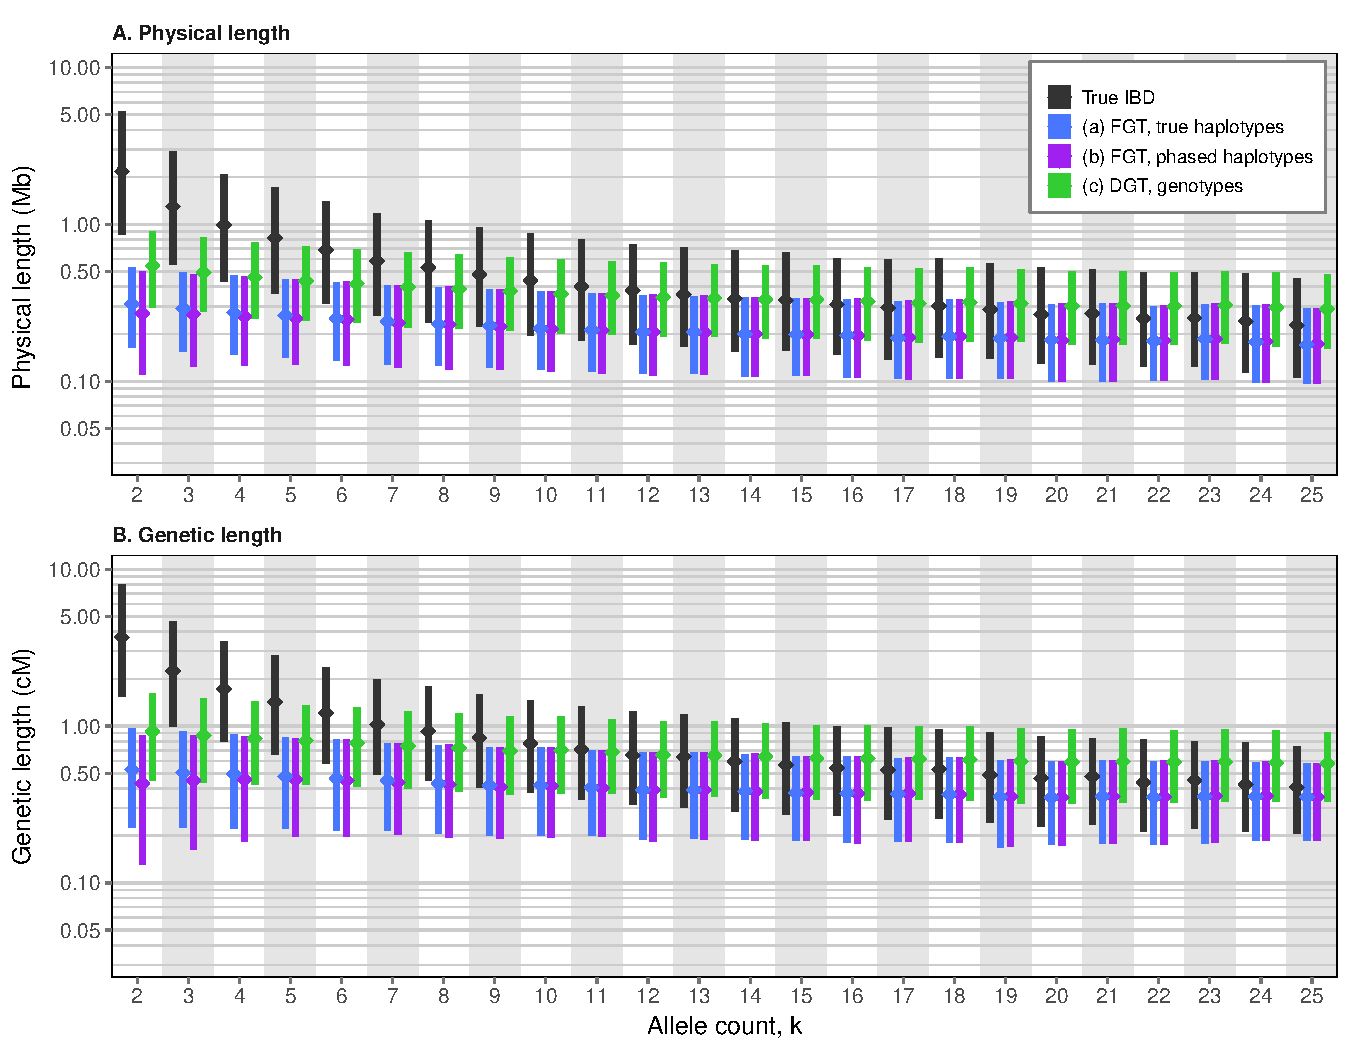
\includegraphics[width=\textwidth]{./img/ch4/length_naive_err.pdf}
\Caption{IBD length distribution using \emph{tidy} after inclusion of genotype error}
{The distribution of physical (A) and genetic (B) segment length is shown by allele count (\fk{}~category).
Results are shown for \n{3} approaches; (a) FGT on true haplotypes, (b) FGT on phased haplotypes, and (c) DGT on genotype data.
Corresponding true lengths are shown in for comparison.
Bottom and top of each bar indicate \nth{1} and \nth{3} quartiles, respectively, between which the median (\nth{2} quartile) is marked (\emph{diamonds}).}
{fig:naive_length_err}
\end{figure}

%

Median physical length (and median genetic length) was relatively short when the \gls{fgt} was used in \cref{A4:fgt_h,,A4:fgt_p}, yielding \SI{0.199520}{\mega\basepair} (\SI{0.381497}{\centi\morgan}) and \SI{0.198376}{\mega\basepair} (\SI{0.378427}{\centi\morgan}), respectively.
For the \gls{dgt}, \cref{A4:dgt}, median length was closer to the true length; \SI{0.331612}{\mega\basepair} (\SI{0.635486}{\centi\morgan}) and \SI{0.337100}{\mega\basepair} (\SI{0.584752}{\centi\morgan}), respectively.
However, for \fk{25}~variants, a clear difference was seen, where the median length was
\SI{0.3114444}{\mega\basepair} (\SI{0.5271301}{\centi\morgan}) in \ref{A4:fgt_h} and
\SI{0.2703742}{\mega\basepair} (\SI{0.4303142}{\centi\morgan}) in \ref{A4:fgt_p}.
But median length was likewise reduced in \ref{A4:dgt} compared to the true length; \SI{0.5431724}{\mega\basepair} (\SI{0.9262646}{\centi\morgan}) and
\SI{2.1723358}{\mega\basepair} (\SI{3.6770937}{\centi\morgan}) respectively.
This difference was not seen towards higher frequencies, \eg at \fk{2}~variants, reaching
\SI{0.1712515}{\mega\basepair} (\SI{0.3543174}{\centi\morgan}),
\SI{0.1725973}{\mega\basepair} (\SI{0.3538201}{\centi\morgan}), and
\SI{0.2886190}{\mega\basepair} (\SI{0.5784379}{\centi\morgan}) in
\ref{A4:fgt_h}, \ref{A4:fgt_p}, and \ref{A4:dgt}, respectively, compared to
\SI{0.2275384}{\mega\basepair} (\SI{0.4081054}{\centi\morgan}) in true segments.

The length distribution of true and detected IBD segments is shown in \cpref{fig:naive_length_err}.
Note the similarity to \ctref{fig:1kg20_lengths}, which was conducted using the \gls{fgt} and \gls{dgt} on data from \gls{1kg} (chromosome~20).
This result suggests that the non-probabilistic IBD detection method implemented in \texttt{tidy} is likely to be biased in presence of genotype error.
To illustrate the problem, consider the example given in \cpref{fig:full_ibd_error}, which highlights the effect of \Correct{error for breakpoint detection using the \gls{fgt} and \gls{dgt}}.
The figure shows the underlying IBD structure for each pair of chromosomes in \n{2} individuals sharing a randomly picked rare allele.
In \cref{fig:full_ibd_error}{a}, the positions of breakpoints detected using the \gls{fgt} and \gls{dgt} are indicated as found along the whole chromosome before the inclusion of error.
In contrast, \cref{fig:full_ibd_error}{b} shows the same analysis but after genotype error was included.
Since the innermost breakpoint interval delimits the inferred IBD segment, it can be expected that even small amounts of genotype error are likely to result in underestimation of IBD length.

%
% !TEX root = ../../main.tex


\begin{figure}[!htb]
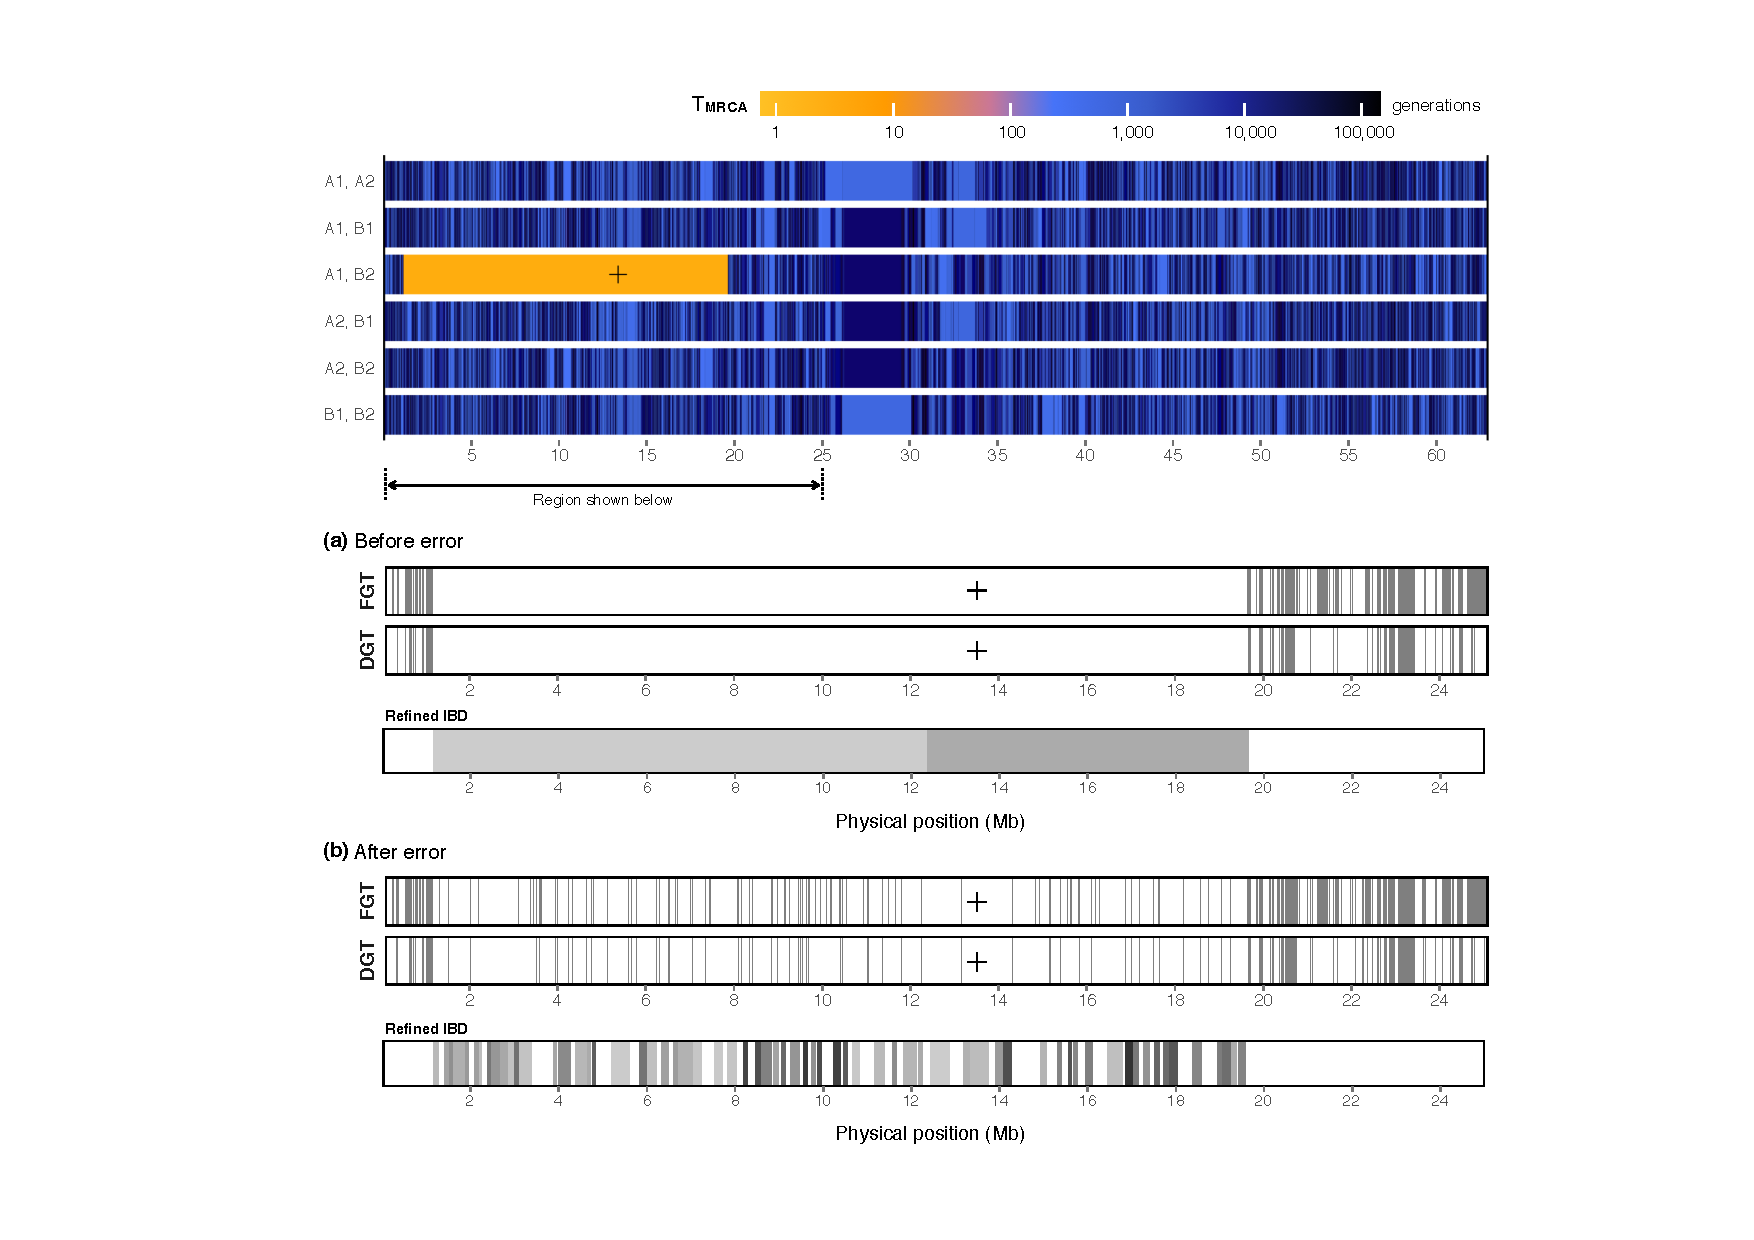
\includegraphics[width=\textwidth]{./img/ch4/full_ibd_error_new}
\Caption{Example of the effect of genotype error on IBD detection}
{One allele and a pair of individuals sharing that allele were randomly selected and the underlying IBD structure for all \n{6} possible pairs of the \n{4} chromosomes was determined from simulation records (\emph{top}).
The figure shows the ``mosaic'' of IBD segments along the sequence of the simulated chromosome; distinguished by the \gls{tmrca}.
The focal shared allele is indicated at the pair of chromosomes sharing that allele (\emph{cross}).
Data were compared before \textbf{(a)} and after \textbf{(b)} the integration of empirically determined genotype error.
In each dataset, the \gls{fgt} and \gls{dgt} were used to detect all breakpoints to the left and right-hand side of the target position.
In addition, the IBD segments reported for the focal pair of haplotypes using the \texttt{Refined\,IBD} method are shown before and after error, where each segment is distinguished by a different colour on grey-scale.
Note that these results were produced on true haplotype data but not phased haplotypes, to highlight the impact of genotype error alone.
Data were simulated using \texttt{msprime} (see \ctref{sec:msprime}).\CorrectLabel}
{fig:full_ibd_error}
\end{figure}

%


%
\subsubsection{IBD detection using \emph{Refined\,IBD} in \emph{Beagle\,4.1}}
%

\CorrectNote{Section re-written to follow the changes made in \cpref{sec:ibd_beagle_tru}}

The probabilistic \texttt{Refined\,IBD} method implemented in \texttt{Beagle} version~4.1 \citep{Browning:2013eh}\footnote{Beagle 4.1: \url{https://faculty.washington.edu/browning/beagle/beagle.html} \accessed{2016}{11}{22}} was used for IBD detection in data after the inclusion of error.
Because the method requires haplotype data, the analysis was performed on the generated (``true'') haplotypes and the set of phased haplotypes; in the following referred to as \cref{A4:fgt_h,,A4:fgt_p}.
The purpose of this analysis was to determine the impact of genotype error on the detection of contiguous shared haplotype intervals.
Because \texttt{Refined\,IBD} attempts to infer IBD for any haplotype pair without reference to a specific target allele, it was necessary to match the set of reported IBD segments to the true shared haplotype intervals that were previously determined from simulation records (\ie all segments around shared \fk{[2,25]} alleles).
The analysis followed the procedure described in \cpref{sec:ibd_beagle_tru}.

\Cref{A4:fgt_h} returned \dec{12.194909}~million segments at \dec{5.807497}~million haplotype pairs.
In \cref{A4:fgt_p}, \dec{12.397767}~million segments at \dec{5.937559}~million haplotype pairs were detected.
In the latter, \n{1382} pairs were removed from the results obtained on phased haplotype data, to enable the analysis to match segments based on the pair of individuals for which IBD was inferred; otherwise the true haplotype pair could not be identified correctly due to the phasing process (as described in \cref{sec:ibd_beagle_tru}).

%
% !TEX root = ../../main.tex


\begin{figure}[!htb]
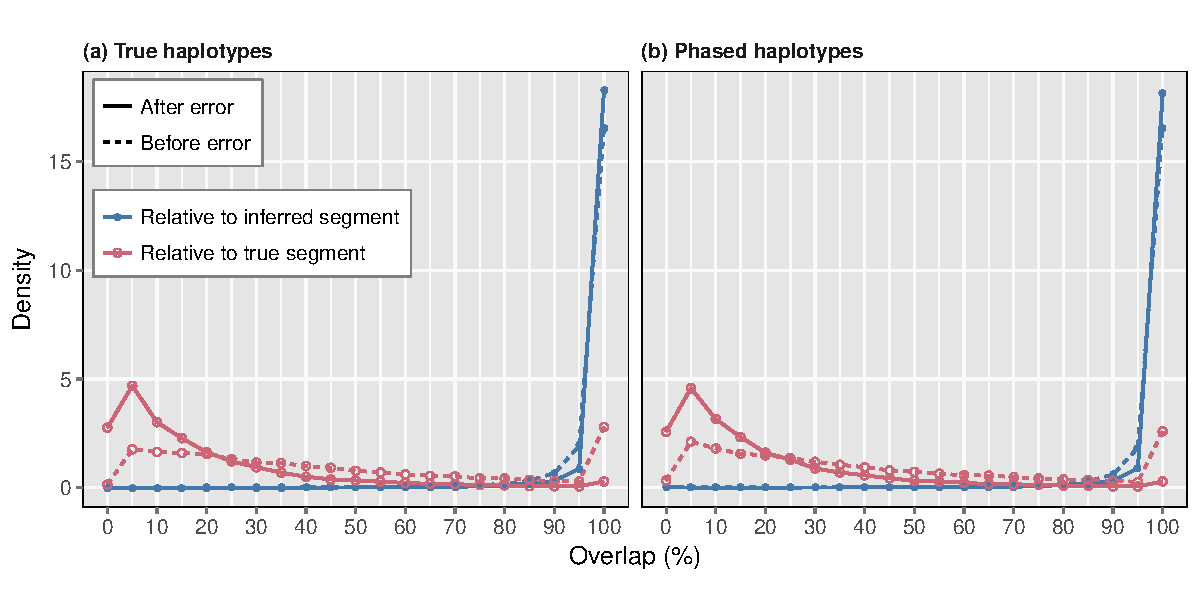
\includegraphics[width=\textwidth]{./img/ch4/beagle_overlap_err}
\Caption{IBD segment overlap inferred using \emph{Refined\,IBD} after integration of error}
{The proportion of overlap was measured by aligning each inferred IBD segment to the set of unique true segments determined for a given pair.
Interval comparisons with zero overlap were ignored.
The results shown were generated on a random subset of \n{10000} pairs in \cref{app:fgt_h,,app:fgt_p}.
The reported densities refer to the proportion of overlap with respect to the inferred segment (\emph{blue}) and the true segment (\emph{red}).
Corresponding densities for the results obtained on data before the integration of error are shown for comparison (\emph{dashed} lines); see \cpref{fig:beagle_overlap}.
\AdditionLabel}
{fig:beagle_overlap_err}
\end{figure}

%

The total base overlap between inferred and true shared haplotype intervals was measured, for which all segments inferred in \ref{A4:fgt_h} and \ref{A4:fgt_p} were aligned to the set of true intervals, after removing duplicate segments in the latter.
The proportion of overlap was measured only at segments at which at least \n{1} base overlapped.
On average, an overlap of \Percent{98.85546} and \Percent{98.5524} was measured relative to inferred IBD in \ref{A4:fgt_h} and \ref{A4:fgt_p}, respectively, but \Percent{18.7064} and \Percent{19.00517} on average when measured relative to true IBD, respectively.
This suggested that the inferred IBD intervals were likely to be found within the region spanned by the underlying shared haplotype, but such that the region was only partially covered on average.
For comparison, before error, average overlap relative to true IBD segments was \Percent{44.29831} and \Percent{42.25553} in \ref{A4:fgt_h} and \ref{A4:fgt_p}, respectively.
The density of overlap measured relative to both the inferred and true segments, before and after error, is shown in \cpref{fig:beagle_overlap_err}.
Also, the example shown in \cpref{fig:full_ibd_error} highlights the difference in coverage for IBD segments inferred using \texttt{Refined\,IBD} on data before and after the integration of error.


Next, inferred IBD segments returned in \cref{A4:fgt_h,A4:fgt_p} were matched to true intervals based on finding a given target site within the inferred interval.
This was done to facilitate measures of accuracy based on the physical distance between a given target site and the position of an inferred breakpoint.
To enable the analysis to measure breakpoint accuracy conditional on the frequency of the target allele, the full set of matched segments was further reduced by removing duplicate segment matches per pair, where the segment tagged by the lowest-frequency allele was retained; again, as described in \cref{sec:ibd_beagle_tru}.
As a result, \dec{1.504609}~million segments and \dec{1.516095}~million segments were retained, respectively, after removing duplicate segment matches per pair.


%
% !TEX root = ../../main.tex


\begin{figure}[!htbp]
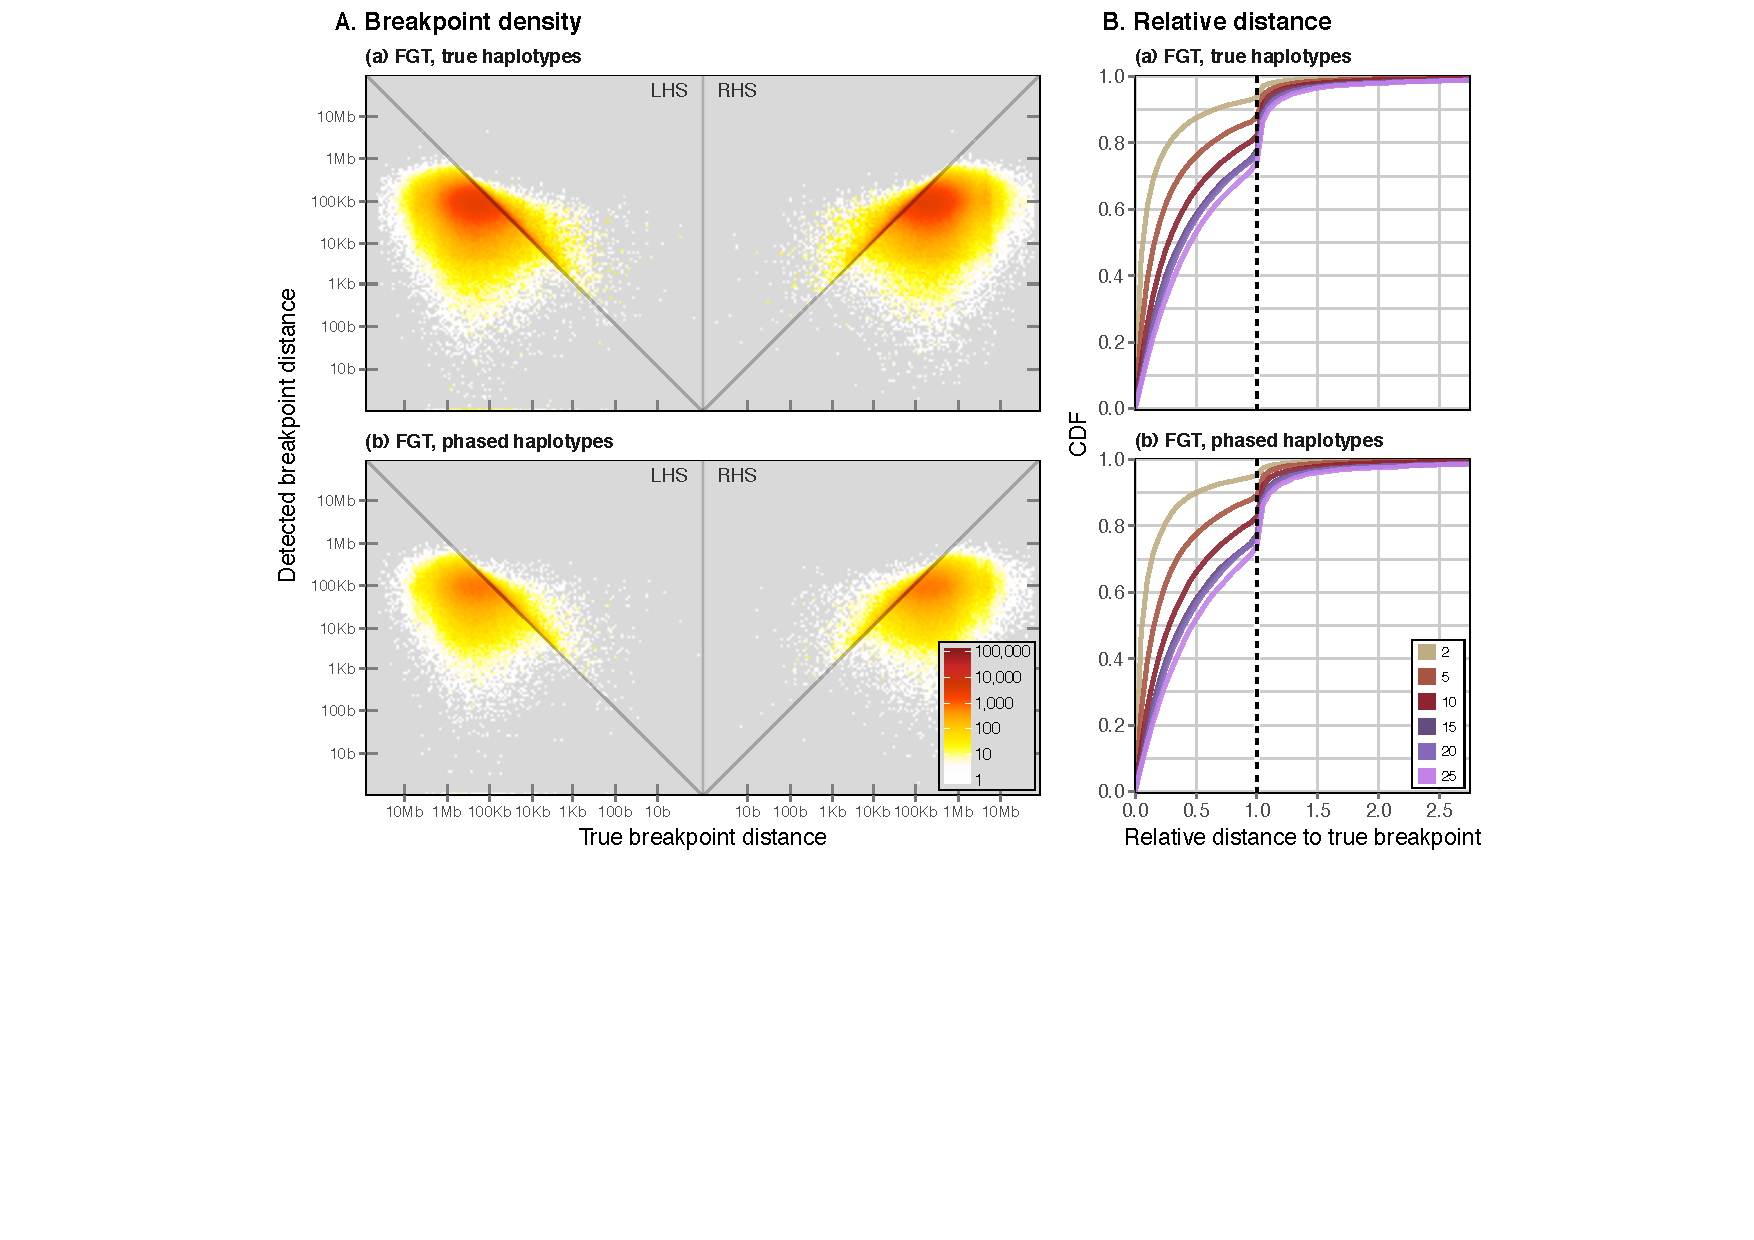
\includegraphics[width=\textwidth]{./img/ch4/break_beagle_err}
\Caption{Accuracy of IBD detection using \emph{Refined\,IBD} after inclusion of genotype error}
{Panel~\textbf{(A)} shows the density of true and detected breakpoints; Panel~\textbf{(B)} shows the physical length in terms of the relative distance between a focal site and the detected breakpoint.
See \cpref{fig:naive_break_err} for a detailed description.}
{fig:beagle_break_err}
\end{figure}

%


In \cref{A4:fgt_h}, \SI{80.10294}{\percent} of the breakpoints detected were underestimated relative to the matched target position.
This was similar in \cref{A4:fgt_p}, where \Percent{80.22851} were underestimated.
A difference between low and high frequency alleles was seen; \Percent{93.73282} and \Percent{95.19862} of segments matched to \fk{2} alleles were underestimated, respectively, while \Percent{75.96449} and \Percent{75.82247} were underestimated at \fk{25} alleles, respectively.
The density of inferred by true breakpoint distance per match segment, as well as the \gls{cdf} of the relative distance per \fk{}~category is shown in \cpref{fig:beagle_break_err}.

The overall accuracy of the breakpoints detected was relatively low;
${r^2=\dec{0.02002049}}$ ($\rmsle=\dec{0.8689641}$) in \ref{A4:fgt_h} and
${r^2=\dec{0.02134879}}$ ($\rmsle=\dec{0.8640695}$) in \ref{A4:fgt_p}, measured by the physical distance between a given target site and the breakpoint on either the left or right-hand side.
Again, accuracy decreased towards lower frequencies; for example, at \fk{2} alleles,
${r^2=\dec{0.005844105}}$ (${\rmsle=\dec{1.4768689}}$) and
${r^2=\dec{0.005439204}}$ (${\rmsle=\dec{1.4941836}}$), respectively, compared to
${r^2=\dec{0.030571264}}$ (${\rmsle=\dec{0.7530622}}$) and
${r^2=\dec{0.032509924}}$ (${\rmsle=\dec{0.7466905}}$) at \fk{25} alleles, respectively.


%
% !TEX root = ../../main.tex


\begin{figure}[!htb]
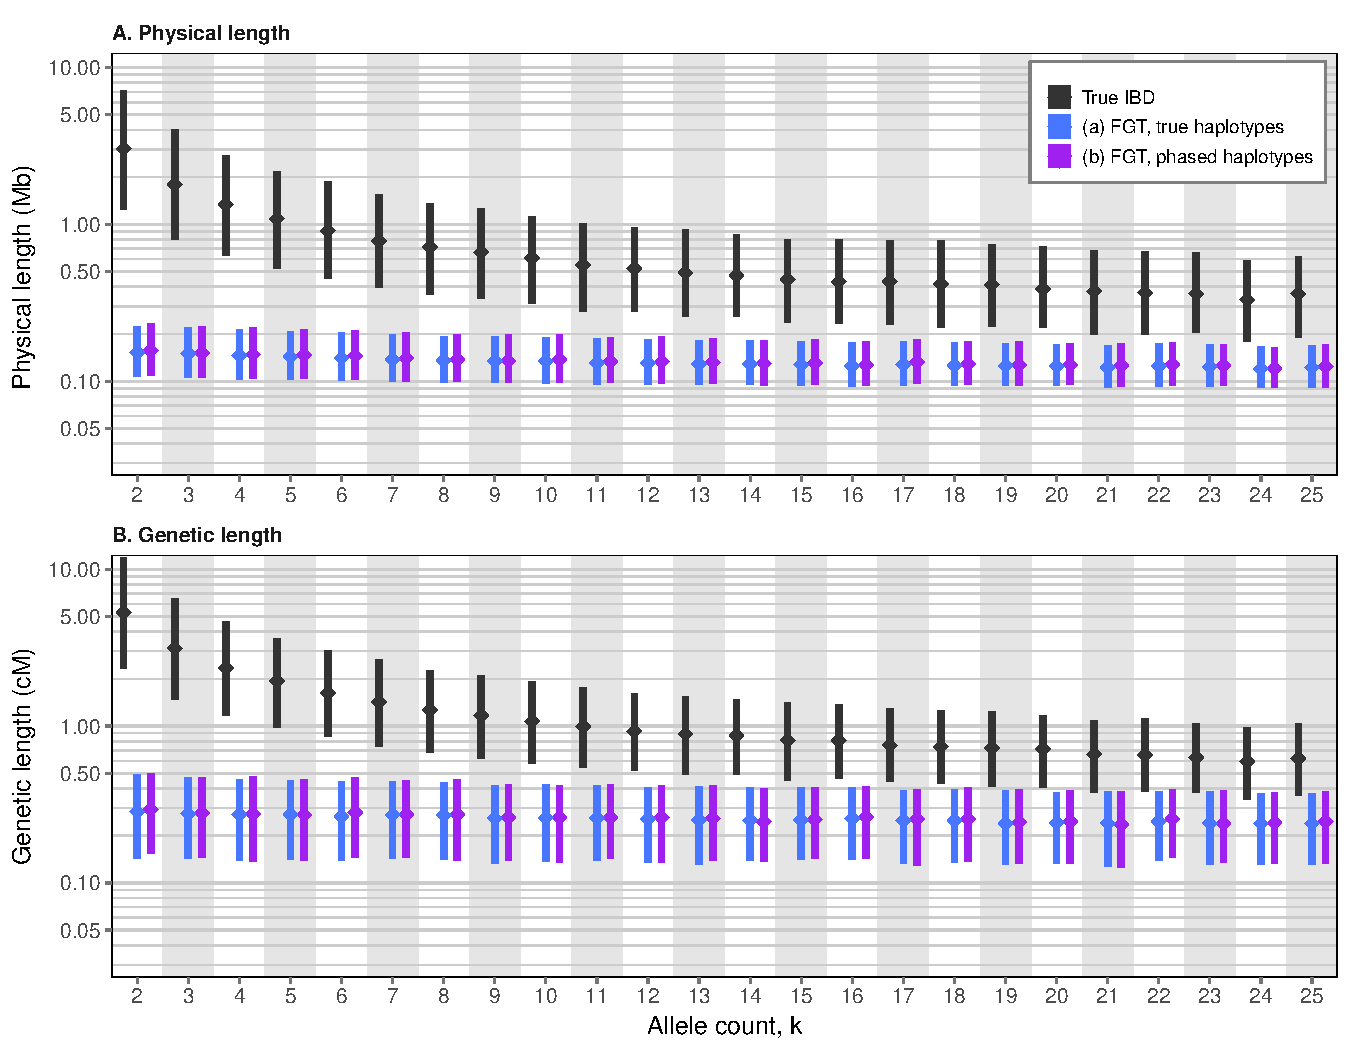
\includegraphics[width=\textwidth]{./img/ch4/beagle_length_err}
\Caption{IBD length detected using \emph{Refined\,IBD} after integration of error}
{The distribution of physical (A) and genetic (B) segment length is shown by allele count (\fk{}~category).
Results were obtained using \texttt{Refined\,IBD} in \texttt{Beagle\,4.1}, on true and phased haplotype data; \ie \cpref{A4:fgt_h,,A4:fgt_p}, respectively.
Bottom and top of each bar indicate \nth{1} and \nth{3} quartiles, respectively, between which the median (\nth{2} quartile) is marked (\emph{diamonds}).\CorrectLabel}
{fig:beagle_length_err}
\end{figure}

%


The physical (genetic) lengths of inferred segments were measured after removing boundary cases;
\n{26856} in \ref{A4:fgt_h} and
\n{26939} in \ref{A4:fgt_p}.
Overall median length was
\SI{0.129056}{\mega\basepair} (\SI{0.2418396}{\centi\morgan}) in \ref{A4:fgt_h} and
\SI{0.130546}{\mega\basepair} (\SI{0.2436294}{\centi\morgan}) in \ref{A4:fgt_p}, which was considerably shorter compared to the set of matched true shared haplotype segments at
\SI{0.518782}{\mega\basepair} (\SI{0.8780738}{\centi\morgan}).
The median length of segments matched to \fk{2} alleles was marginally longer compared to higher-frequency alleles;
\SI{0.1546400}{\mega\basepair} (\SI{0.2722529}{\centi\morgan}) in \ref{A4:fgt_h} and
\SI{0.1583120}{\mega\basepair} (\SI{0.2707016}{\centi\morgan}) in \ref{A4:fgt_p}, where the matched true segments were found at
\SI{2.6124460}{\mega\basepair} (\SI{4.4754927}{\centi\morgan}).
For \fk{25} alleles, median length was
\SI{0.1233630}{\mega\basepair} (\SI{0.2291572}{\centi\morgan}) and
\SI{0.1251330}{\mega\basepair} (\SI{0.2309485}{\centi\morgan}), respectively, compared to
\SI{0.3965520}{\mega\basepair} (\SI{0.6371054}{\centi\morgan}) for the matched true segments.
The distribution of segment length inferred in \cref{A4:fgt_h,,A4:fgt_p} is shown in \cpref{fig:beagle_length_err}.



%
%%% Replaced with above
%
% , \SI{79.52689}{\percent} overestimated, and \SI{0.111050}{\percent} coincided with true IBD breakpoints.
% This distribution was similar in \cref{A4:fgt_p}, yielding \SI{20.26241}{\percent}, \SI{79.64156}{\percent}, and \SI{0.096028}{\percent}, respectively.
% This is also seen in \cpref{fig:beagle_break_err}, where IBD breakpoints tend to be underestimated
% In comparison to IBD detected using \texttt{tidy}, overall accuracy was lower, with ${r^2=0.017126}$ in \ref{A4:fgt_h} and ${r^2=0.017756}$ in \ref{A4:fgt_p}, and the magnitude of error more elevated, at ${\rmsle=0.8496714}$ and ${\rmsle=0.8441583}$, respectively.
%
% After removing boundary cases,
% \SI{0.2707015}{\percent} and \SI{0.2865119}{\percent} in \ref{A4:fgt_h} and \ref{A4:fgt_p} respectively, median length was further reduced in comparison to \texttt{tidy}, which was observed at \SI{0.1291382}{\mega\basepair} (\SI{0.2527802}{\centi\morgan}) in \ref{A4:fgt_h} and
% \SI{0.1313005}{\mega\basepair} (\SI{0.2561401}{\centi\morgan}) in \ref{A4:fgt_p};
% true length was noticeably longer with \SI{0.4959440}{\mega\basepair} (\SI{0.8832682}{\centi\morgan}); note that this was the median length found for the same set of segments as matched in \ref{A4:fgt_h}.
% The distribution of true and detected IBD length is given in \cpref{fig:beagle_length_err}.
%


%
\subsection{Discussion}
%

Two conclusions can be drawn from the analysis of simulated data after the integration of (realistic) error rates.
First, the distribution of shared alleles is altered in presence of error such that a given shared allele may not correctly identify genomic regions of recent shared ancestry between pairs of haplotypes.
In cased where a rare allele was missed (or removed through quality control), the underlying shared haplotype segment may still be retrieved from other, nearby rare variants that identify the same shared haplotype in a given haplotype pair.
\Addition{Conversely, in cases where a rare allele was falsely called or typed, it can be expected the the actual relationship between the haplotypes at that position is relatively old, such that the interval detected is likely to be relatively short.}

Second, the main insight gained from the analyses using the \gls{fgt}, \gls{dgt}, and \texttt{Refined\,IBD} is that the impact of error on the detection of shared haplotype segments is dramatic.
As highlighted by the example shown in \cpref{fig:full_ibd_error}, neither method was able to infer contiguous intervals that accurately reflect the actual shared haplotype segment.
When the \gls{fgt} or \gls{dgt} were used, it was suggested that even low rates of error may lead to the observation of false positive breakpoints, because even one false positive would suffice to disrupt the rule-based detection process as it is currently implemented.

% disrupt the IBD detection process and is likely to result in a general underestimation of the underlying IBD length.
% Therefore, the analysis has provided sufficient evidence to justify the development of a more extensive method for IBD detection.
% In particular, I used the the estimated proportions of genotype \Correct{error} to extend the targeted IBD detection approach such that the distribution of genotype pairs can be modelled for inference under IBD and non-IBD.
% From this, a novel, fully probabilistic approach was developed using a \gls{hmm}.

\Addition{However, when using \texttt{Refined\,IBD}, the low overall accuracy measured may not be surprising given that the inferred segments were likely to be scattered along the full length of the underlying shared haplotype region.
The matching process was therefore not straightforward, as only the segment covering a given target site was retained.
For example, an additional method could be implemented to concatenate neighbouring segments inferred per pair to approximate the interval of the underlying shared haplotype.
This was not attempted here, as it appeared more feasible to extend the targeted IBD detection approach implemented in \texttt{tidy}, which was done in the following section.}



%
\section{A Hidden Markov Model for IBD inference}
\label{sec:ibd_hmm_method}
%

Despite the high accuracy of the \gls{fgt} and \gls{dgt} to detect shared haplotype segments in simulated data, it has emerged from the previous analysis that a non-probabilistic approach may be less suitable for IBD detection if the presence of genotype error cannot be excluded.
Because it cannot be assumed that real data is obtained without error, it would therefore be beneficial to devise a fully probabilistic implementation of the IBD detection algorithm, in which observed error rates can be included.
Here, this was attempted by constructing a \glsentryfull{hmm}.

An \gls{hmm} is a probabilistic sequence model which is widely used in applications of machine learning, likelihood computation, and sequence classification; see \citet{Rabiner:1989hs}.
In general, a sequence of observations is assumed to be the product of an unobserved Markov process, in which a sequence of underlying, but ``hidden'' states determines the probability of observing the data.
Each state is characterised by a probability distribution over a finite set of possible observations.
Although the sequence of hidden states is not known, it can be inferred from the sequence of observations.

A wide range of statistical methods for genetic data analysis are driven by \gls{hmm}-based algorithms.
Notable examples are methods used for genotype phasing and imputation; \eg \texttt{SHAPEIT} \citep{Delaneau:2011iu},
\texttt{EAGLE} \citep{loh2016fast,Loh:2016bl}, and
\texttt{IMPUTE} \citep{Howie:2009hq,Howie:2011ji}, to name a few.
It is worth to mention that many of the commonly employed methods (above included) are based on the influential \citet{Li:2003uz} model, which for a set of observed genotypes reconstructs the unobserved haplotypes as ``imperfect mosaics'' of known haplotypes in reference data.
While this model provides the ability to solve several kinds of problems in statistical genetics, such as phasing or imputation, it is less applicable for inference of IBD.

A variety of different approaches exist for the inference of IBD segments, many of which have not fully adopted the view that observed genetic variation is the product of a genealogical process which, in principle, can be modelled as a Markov process.
An example of a rule-based method is the widely implemented \texttt{GERMLINE} algorithm \citep{Gusev:2009hd}, which is part of the often employed \texttt{Refined\,IBD} method \citep{Browning:2013eh}.
This algorithm was designed as an efficient search method through which IBD status is inferred from imperfectly matched haplotypes in large sample data.
In contrast, model-based implementations for inference of IBD in samples of seemingly unrelated individuals all rely on \glspl{hmm}; see review by \citet{Thompson:2013cj}.
The first to assume that IBD arises from a Markov process (without specifically stating it) was \citet{Stam:1980gs}, who extended the idea of recombination breakpoints (or ``junctions'') introduced by \citet{Fisher:1949vh,fisher1954} to describe the probability distribution of the fraction of the genome that is identical by descent in a finite and randomly mating population.
% Later, \citet{Chapman:2003jt} proposed a different model to describe the length of IBD segments in terms of the distribution of recombination breakpoints along pairs of chromosomes as a Markov chain.
Later, \citet{Leutenegger:2003is} developed an \gls{hmm} for inference of inbreeding coefficients from genotype data in individuals of unknown parental relationships.
Equivalent models were implemented to detect IBD in phased haplotypes \citep[\eg][]{Purcell:2007dg,Browning:2008es}.

Here, a different IBD-model is proposed which is used for inference of recombination breakpoints around a target position in pairs of individuals.
The approach is conceptually similar to the previously presented method for deterministic IBD detection using the \gls{fgt} or \gls{dgt}, see \cpref{sec:tidy}, but where the detection of breakpoint intervals (\ie the physical start and end points of IBD segments) are determined through sequence classification in the \gls{hmm}.
Notably, the presented method relies on genotype information and does not require haplotype data; it is therefore not affected by phasing error.

The following section describes the algorithm through which target sites in sample data are analysed.
This is followed by a detailed description of the model, which includes the theoretical expectations under the assumption of no error.
Then, the model is extended to include the empirically determined distributions of genotype error for each of the possible genotype pairs.
In the end, the presented \gls{hmm}-based method for IBD detection was evaluated in the same way as was done for the \gls{fgt} or \gls{dgt} in the previous chapter.
%The \gls{hmm} was evaluated on simulated data and applied to a real dataset.


%
\subsection{The algorithm for probabilistic IBD inference}
%


Consider a sample of $N$ diploid individuals and $M$ variant markers; in particular, \gls{snp} data are assumed.
To determine the IBD structure around a focal variant site, let this site be denoted by ${i \in \lbrace 1, \ldots, M \rbrace}$ and its physical position by $b_i$.
All individuals sharing the derived (alternate) allele at this site are identified and analysed in a pairwise fashion.
In each pair, the breakpoint interval, ${[b_L, b_R]}$, is inferred, where $b_L$ and $b_R$ are the chromosomal positions of the most likely recombination breakpoints to the left and right-hand side of the focal position, respectively.

As before, it is convenient to refer to a target site by its frequency in the sample.
Thus, \fk{} variants are distinguished where $k$ is the number of allele copies in the sample, and where ${k \geq 2}$ must be satisfied.
Note that only those individuals are considered that are heterozygous for the focal allele, which is why the subset of identified individuals may be smaller than $k$, but not smaller than 2 in order to form at least \n{1} pair.
Also, as described in Chapter~3 (\ccref{sec:rarevars}), rare variants are presumed to derive from relatively recent mutations and are therefore more likely to identify long IBD tracts, as recombination had less time to break down the length of the shared haplotype identity.
Hence, this method is primarily intended for inference of IBD around rare variants, where ${k \ll 2N}$.
However, note that in principle any \fk{\geq2} variant can be analysed using the presented method.

The input data analysed in the \gls{hmm} is the paired sequence of genotypes in both individuals sharing the focal allele.
The observation sequence is composed of the paired genotypes along the chromosomes of the \n{2} individuals sharing the focal allele; as such, haplotype data is not required.
Since each individual contributes a genotype at a single locus, $g_k$ (where ${k \in \lbrace 0,1,2 \rbrace}$), to form a genotype pair, denoted by $g_{k_1 k_2}$, it follows that there are \n{6} possible observation states; $g_{00}$, $g_{01}$, $g_{02}$, $g_{11}$, $g_{12}$, and $g_{22}$, where the order of genotypes in a pair is ignored.
Further, \n{2} states are distinguished in which genotype pairs can be observed; either the \n{2} individuals share a haplotype identical by descent, or they do not, which is denoted by \emph{ibd} and \emph{non}, respectively.
These correspond to the hidden states that are assumed to generate the data.

For a given focal site and a pair of individuals sharing the allele, the sequence of genotype pairs is analysed as \n{2} independent Markov chains; \ie \n{1} to the left and \n{1} to the right-hand side of the focal variant, with the focal site at the start of both chains.
For convenience, the index~$j$ is defined relative to $i$ and follows the direction of moving from $b_i$ to the last site in the observed sequence, either $b_1$ to the left or $b_M$ to the right-hand site.
Hence, ${j=0}$ at the focal site and ${j = m}$ at the last site, where $m$ is the number of markers to the left or right-handed sequence relative to the focal site (excluding the focal site).

Since the focal allele is assumed to identify the shared haplotype in \emph{ibd}, the first site along the sequence that is classified in the \emph{non} state is taken as a breakpoint, on both sides, such that the inferred IBD segment is enclosed in ${[b_L, b_R]}$.
By definition, the smallest detectable interval around a focal variant at site $i$ is therefore ${[b_{i-1}, b_{i+1}]}$.
If the chain remains in \emph{ibd} until the end of the sequence, the last position is taken as a breakpoint (referred to as a \emph{boundary case}).

The following section describes the underlying model through which each site in the observation sequence is classified into either \emph{ibd} or \emph{non}.


%
\subsection{Description of the model}
%

\Glsentrylong{ibd} is modelled as a first-order Markov process in a \n{2}-state \gls{hmm}, where the observed genotypes in a pair of diploid individuals are emitted from either the \emph{ibd} or the \emph{non} state.
Given the Markov property, the following assumptions are made.
First, the probability of the hidden state at site~$j$ only depends on the previous hidden state at site~${j-1}$.
Second, the probability of observing a particular genotype pair at site~$j$ only depends on the hidden state at site~$j$ and not on any of the other states.

Let the hidden state space be denoted by ${S = \lbrace \textit{ibd},\textit{non} \rbrace}$, and the set of observable states by ${G = \lbrace g_{00},~g_{01},~g_{02},~g_{11},~g_{12},~g_{22} \rbrace}$.
The model itself is denoted by
\begin{equation}\label{eq:hmm_model}
	\lambda ~=~ \lbrace \Psi, \xi, \pi \rbrace
\end{equation}
where $\Psi$ is a matrix of state \emph{transition} probabilities and $\xi$ corresponds to a set of vectors which store the probability of observing each of the possible genotype pairs; \ie the \emph{emission} probabilities in each state.
The model is illustrated in \cpref{fig:info_hmm}, where the probabilities of emission from \emph{ibd} are denoted by $\delta_{k_1 k_2}$ and from \emph{non} by $\eta_{k_1 k_2}$.
The \emph{initial} probabilities of being in either state at the start of the sequence is given by $\pi$.

%
%!TEX root = ../../main.tex


\begin{figure}[!htb]
\centering
%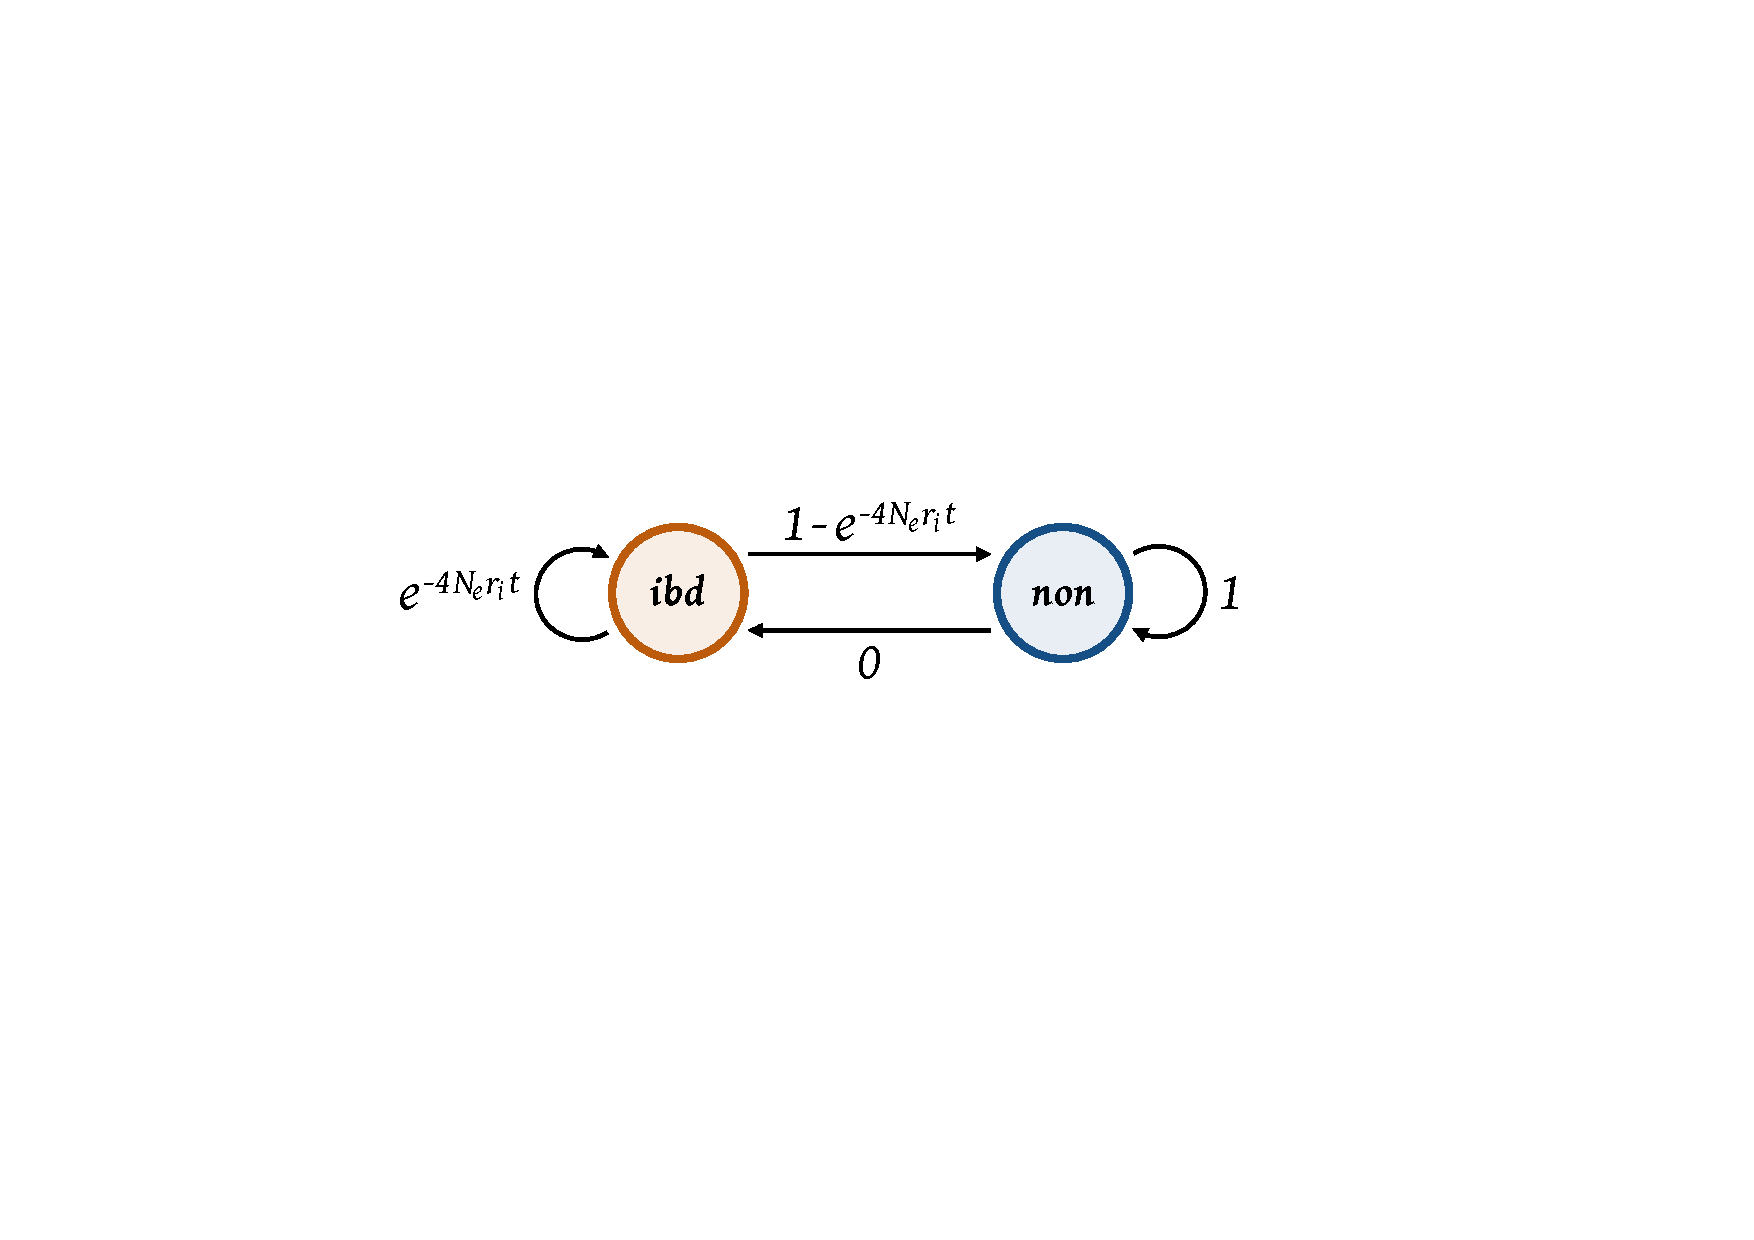
\includegraphics[width=0.75\textwidth]{./img/ch4/hmm_trans}\\

\vspace{5pt}
\begin{tikzpicture}[->,>=stealth,auto,thick,
txt/.style={font=\sffamily\small,text width=2.5cm},
sub/.style={circle,draw=white, fill=white,minimum size=1.75cm},
state/.style={circle,draw,ultra thick,minimum size=1.5cm,outer sep=2pt,font=\bfseries\Large},
dbl/.style={diamond,draw=black!50,thick,minimum size=1.45cm,outer sep=2pt},
obs/.style={diamond,draw=black,fill=white,fill opacity=0.5,text opacity=1,thick,minimum size=1.5cm,outer sep=2pt,font=\bfseries}]

\newcommand{\observeIBD}[4]{
\draw[->,draw=DarkOrange2!20,ultra thick] (#1) to (#2);
\draw[->,draw=DarkOrange3,densely dotted] (#1) -- (#2) node [pos=#4,sloped,left,fill=white,font=\small,inner sep=1pt] {#3};
}
\newcommand{\observeNON}[4]{
\draw[->,draw=DodgerBlue3!20,ultra thick] (#1) to (#2);
\draw[->,draw=DodgerBlue4,densely dotted] (#1) -- (#2) node [pos=#4,sloped,right,fill=white,font=\small,inner sep=1pt] {#3};
}

\node[txt] at (-1, 5) {Hidden\\states, $S$};
\node[txt] at (-1, 0) {Observation\\states, $G$};

\node[sub] (I) at (3.5,5) {};
\node[sub] (N) at (8.5,5) {};

\node[state,draw=DarkOrange3,fill=DarkOrange1!25] (ibd) at (3.5,5) {\emph{ibd}};
\node[state,draw=DodgerBlue4,fill=DodgerBlue1!25] (non) at (8.5,5) {\emph{non}};

% \node[dbl] (s00) at (1,0.84) {};
% \node[dbl] (s01) at (3,0.84) {};
% \node[dbl] (s02) at (5,0.84) {};
% \node[dbl] (s11) at (7,0.84) {};
% \node[dbl] (s12) at (9,0.84) {};
% \node[dbl] (s22) at (11,0.84) {};

\node[obs] (g00) at (1,0) {$g_{00}$};
\node[obs] (g01) at (3,0) {$g_{01}$};
\node[obs] (g02) at (5,0) {$g_{02}$};
\node[obs] (g11) at (7,0) {$g_{11}$};
\node[obs] (g12) at (9,0) {$g_{12}$};
\node[obs] (g22) at (11,0) {$g_{22}$};

% \path (ibd.25)  edge node[above]{\Large{${1 - e^{-4 \Ne r_i \tau_k}}$}} (non.155);
\path (ibd.25)  edge node[above]{\large{$\varphi$}} (non.155);
\path (non.205) edge node[below]{\large{$0$}} (ibd.335);

% \path (ibd) edge [out=205,in=155,looseness=5] node[left] {\Large{${e^{-4 \Ne r_i \tau_k}}$}} (ibd);
\path (ibd) edge [out=205,in=155,looseness=5] node[left] {\large{$1-\varphi$}} (ibd);
\path (non) edge [out=25,in=335,looseness=5] node[right] {\large{$1$}} (non);

\observeIBD{I.315}{g22}{$\delta_{22}$}{0.25}
\observeIBD{I.300}{g12}{$\delta_{12}$}{0.31}
\observeIBD{I.285}{g11}{$\delta_{11}$}{0.4}
\observeIBD{I.270}{g02}{$\delta_{02}$}{0.5}
\observeIBD{I.255}{g01}{$\delta_{01}$}{0.45}
\observeIBD{I.240}{g00}{$\delta_{00}$}{0.45}

\observeNON{N.225}{g00}{$\eta_{00}$}{0.25}
\observeNON{N.240}{g01}{$\eta_{01}$}{0.31}
\observeNON{N.255}{g02}{$\eta_{02}$}{0.4}
\observeNON{N.270}{g11}{$\eta_{11}$}{0.5}
\observeNON{N.285}{g12}{$\eta_{12}$}{0.45}
\observeNON{N.300}{g22}{$\eta_{22}$}{0.45}

\end{tikzpicture}
% \vspace{10pt}
%
% X
%
% \vspace{10pt}
% \begin{tikzpicture}[auto,thick,decoration={coil},
% line/.style={->,>=latex},
% rec/.style={->,>=stealth,rounded corners=4pt},
% txt/.style={font=\sffamily\small,text width=2.5cm},
% dna/.style={decorate,thick,decoration={aspect=0, segment length=0.5cm}},
% var/.style={rectangle,draw=black!50,fill=black!10,minimum size=0.4cm,outer sep=2mm,inner sep=2pt,font=\tiny\sffamily\bfseries}]
%
% \node[txt] at (-1, 5) {Genome};
% \node[txt] at (-1, 3.5) {Sample variant sequence};
%
% % \node[var] at (2.1,0) {};
% % \node[var] at (3.5,0) {};
%
% \foreach \v [remember=\v as \last (initially 1), count=\i] in {1.94,2.87,4.05,4.71,5.86,7.37,8.63,9.66,10.38}{
% 	\fill[gray!50] (\v - 0.05,4.6) rectangle (\v + 0.05,5.4);
% 	\coordinate (beg) at (\v,4.4);
% 	\node[var]  (end) at (\v,3.4) {\i};
% 	\draw[line] (beg) to (end.north);
% }
%
% \draw[dna, decoration={amplitude=.15cm}] (1.1,5) -- (11.5,5);
% \draw[dna, decoration={amplitude=-.15cm}] (1,5) -- (11.5,5);
%
% \fill[white] (0.9,4.6) rectangle (1.13,5.4);
% \fill[white] (11.2,4.6) rectangle (11.6,5.4);
%
% % \node[site] (1) at (1.0,2) {};
% %
% % \foreach \s [remember=\s as \last (initially 1)] in {2,...,10}{
% %   \node[site] (site\s) at (\s,2) {};
% %   \draw[line] (\last,2) to (site\s.west);
% % 	\node[site] (\s) at (\s,2) {};
% % }
%
% \end{tikzpicture}

\vspace{5pt}

\Caption{Illustration of the Hidden Markov Model for IBD inference}%
{\N{2} hidden states are assumed to generate the observations in a Markov process; \emph{ibd} and \emph{non}.
Transitions from each state into any state are indicated by \emph{solid} lines.
The probability of transition from \emph{ibd} to \emph{non} is denoted by $\varphi$, and from \emph{non} to \emph{ibd} is set to zero; hence, once the Markov chain proceeds into the \emph{non} state it cannot transition back into \emph{ibd}.
This is because the IBD process is modelled such that only the innermost IBD segment is inferred, relative to the focal position which sits at the start of the sequence.
The input sequence consists of genotype data from a pair of individuals, resulting in \n{6} possible observation states; denoted by $g_{k_1 k_2}$, where ${k_1,k_2 \in \lbrace 0,1,2 \rbrace}$.
The probabilities of emitting each possible genotype pair given each hidden state are denoted by $\delta_{k_1 k_2}$ and $\delta_{k_1 k_2}$ for \emph{ibd} and \emph{non}, respectively; indicated by the \emph{dotted} lines.
The direction of arrows indicates conditional dependence; \ie the transition from one hidden state into another state, or emission of a genotype pair while being in \emph{ibd} or \emph{non}.}%
{fig:info_hmm}
\end{figure}

%

The parameters of the model are defined in \n{2} ways.
First, theoretical expectations for transition, emission, and initial probabilities are derived; see \pref{sec:HmmTrans,,sec:HmmEmiss,,sec:HmmInit}, respectively.
Then, in \cpref{sec:HMMError}, the model is extended to include genotype error from empirical data as obtained in \cpref{sec:generrprofiles}.




%
\subsubsection{Transition probabilities}
\label{sec:HmmTrans}
%

Given the \n{2} hidden states, the transition matrix $\Psi$ is defined as a $2 \times 2$ matrix which stores the probabilities of moving from one state into another state, as well as the probabilities of remaining in the same state; see below.
\begin{equation}\label{eq:transmatrix}\onehalfspacing
\Psi_{j,k}  ~=~
\begin{bmatrix}
	\psi_{j,k}(\textit{ibd}\mid\textit{ibd})  &
	\psi_{j,k}(\textit{non}\mid\textit{ibd})  \\[1ex]
	\psi_{j,k}(\textit{ibd}\mid\textit{non})  &
	\psi_{j,k}(\textit{non}\mid\textit{non})  \\
\end{bmatrix}
\end{equation}
In particular, the probability of transition from \emph{ibd} to \emph{non}, denoted by ${\varphi = \psi_{j,k}(\textit{non}\mid\textit{ibd})}$, is modelled dependent on the rate of recombination between consecutive sites, in order to estimate the probability of the distance to the first recombination breakpoint along the sequence.
\N{2} variables are considered; the genetic distance between the current and the previous position, and the expected \gls{tmrca} of the focal \fk{} variant.

Let the genetic distance between positions $b_j$ and $b_{j-1}$ be denoted by $r_j$, measured in \emph{Morgan}, which is the product of the recombination rate per site per generation, $\rho$, and the physical distance of the sequence interval in basepairs.
If the recombination rate varies over the length of the chromosome, that is if a genetic map is available, $r_j$ can be obtained from map distances.
Note that the model considers ${2 r_j}$ to account for recombination occurring along either of the \n{2} lineages considered.
In a population genetics setting, time is scaled in units of $2\Ne$ generations for a sample of diploid individuals, where \Ne is the diploid effective population size of the population under consideration.
% \N{1} time unit therefore is ${\tau = \rfrac{t}{2\Ne}}$, where $t$ corresponds to time measured in discrete generations.
Thus, the scaled rate of recombination within the interval between consecutive sites and per time unit is equal to ${4\Ne r_j}$.

The expected age of an allele, measured in scaled time units and denoted by $\tau_k$, can be estimated directly from its frequency; \Correct{as already presented in \cpref{sec:alleleage}.}
\Correct{Briefly,} \citet{Kimura:1973ug} derived a formulation for the expected age of a selectively neutral allele in a stationary population using diffusion theory; \Correct{see \cref{eq:intro_kimura_ohta}.}
Later, \citet{Griffiths:2013ec} showed that the expected age of an allele in a constant population can be derived in context of the coalescent, given the assumptions of the infinite sites model; \Correct{see \cref{eq:intro_griffiths_tavare}.}
Both approaches result in approximately equal distributions for allelic age
\Addition{with negligible differences; \eg for a sample of ${n=\num{1000}}$ haplotypes, the expected age of an \fk{2} allele is
${\mathbb{E}\left[t_m\right]=\dec{0.02490825}}$ using \cref{eq:intro_kimura_ohta} and
${\mathbb{E}\left[t_m\right]=\dec{0.02398986}}$ using \cref{eq:intro_griffiths_tavare}.
}
Here, \cref{eq:intro_kimura_ohta} was used for computation of $\tau_k$ due to its simplicity.

\Addition{It should be noted that the expectation of allele age as used here implies the assumption of a constant population size, which is rarely observed in nature and also not the case for the simulated dataset on which the presented method was evaluated (as presented further below).
The value of the expected age is nonetheless useful to arrive at approximate transition probabilities that are assumed to be suitable for the current \gls{hmm}.}

The distance to a recombination event follows the geometrical distribution if measured in discrete generations.
However, it can be approximated on a continuous time scale using the exponential distribution in the limit as $\Ne$ tends to infinity; that is, generally, if population size is sufficiently large \citep[see][]{hein2004gene}.
Thus, the probability of transition from \emph{ibd} to \emph{non} can be expressed as follows.
\begin{equation}\label{eq:hmm_trans_prob}
	\varphi ~=~ \psi_{j,k}(\textit{non}\mid\textit{ibd}) ~=~
	1 - \Big( 1 - \frac{4\Ne r_j}{2\Ne} \Big)^{2\Ne\tau_k} ~\approx~
	1 - \euler{-2\Ne r_j \tau_k}
\end{equation}
The probability of remaining in \emph{ibd} is therefore ${\psi_{j,k}(\textit{ibd}\mid\textit{ibd}) = 1-\varphi}$, because the probability distribution over possible states for a given state must sum to~1.
For illustration, \cpref{fig:hmm_transmatrix} shows the probability of transition from \emph{ibd} dependent on the genetic distance between consecutive sites along the sequence and the allele frequency of the focal allele.

Note that the model relies on the assumption that the probability of transition from \emph{non} to \emph{ibd} has \n{0} probability; \ie
\begin{equation*}\onehalfspacing
	\psi_{j,k}(\textit{ibd}\mid\textit{non}) = 0\ , \quad
	\psi_{j,k}(\textit{non}\mid\textit{non}) = 1\ .
\end{equation*}
Therefore, the architecture of the model is not fully connected or \emph{ergodic}.
This is typically referred to as a left-to-right or \emph{Bakis} \gls{hmm}, as transitions can only proceed in \n{1} direction.
Once the \emph{ibd} state has been left, the chain remains in the \emph{non} state such that only the innermost IBD segment is inferred, relative to the focal site at the start of the sequence.

%
% !TEX root = ../../main.tex


\begin{figure}[!htb]
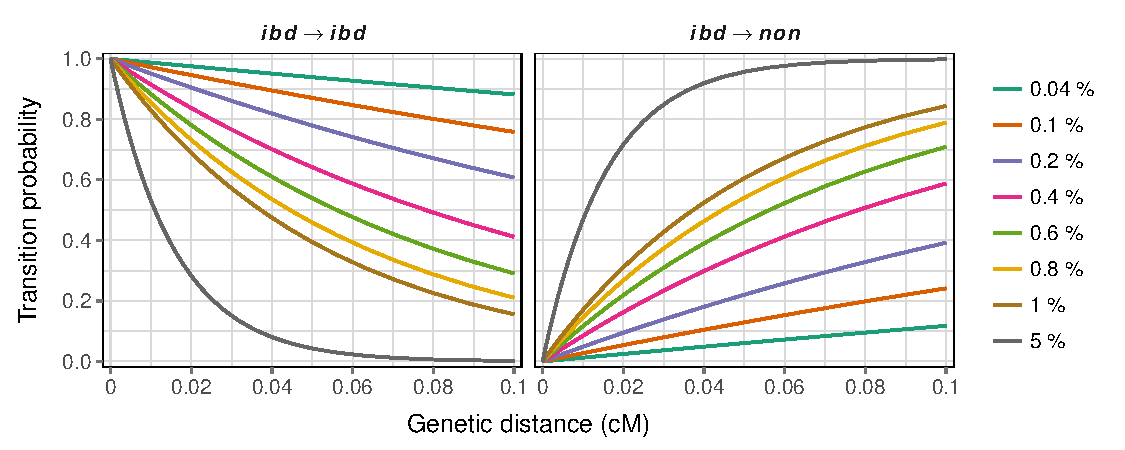
\includegraphics[width=\textwidth]{./img/ch4/hmm_transmatrix}
\Caption{Probability distribution of transition dependent on IBD}
{The probability of transition was modelled dependent on the genetic distance between a particular site and the previous site and the expected age of the focal allele.
The frequency of the focal allele determines its expected age, which is shown for different frequency values.
An effective population size of ${\Ne = \num{10000}}$ was specified.
For example, the frequency of a \fk{2} allele in a sample of \n{5000} haplotypes is equal to 0.04\% (\emph{green} line).}
{fig:hmm_transmatrix}
\end{figure}

%

It is necessary to note that a pair of diploid individuals may share more than \n{1} recent haplotype identical by descent; \eg along the same \n{2} chromosomes or any pair of the \n{4} chromosomes.
Here, this possibility was not considered due to the variant-centric approach of the method.
As such, inference is dependent on the properties of a given \fk{}~variant.
The focal allele serves as an indicator for haplotype sharing and transition probabilities are computed dependent on the expected time of the focal mutation event, given the allele frequency at the focal site.
For example, by allowing transitions from the \emph{non} state back to \emph{ibd},
the IBD inference would be biased as the length of distinctly inferred segments (\ie for other genealogies along the chromosome) would be conditioned on the expected age of the focal allele.


%
\subsubsection{Emission probabilities}
\label{sec:HmmEmiss}
%

\CorrectNote{This section was simplified according to the comments provided.}

The model parameter $\xi$ stores the emission or \emph{output} probability vectors of the hidden states.
Each vector is a probability distribution over the possible observation states with sum~1.
There are \n{6} possible states in which a pair of genotypes can be observed.
A genotype pair is denoted by ${g_{k_1,k_2}}$, where ${k_1,k_2 \in \{0,1,2\}}$.
In the following, the emission probabilities for the possible genotype pairs are derived for each hidden state; \emph{non} and \emph{ibd}.
The probability to observe a given genotype pair is written as ${P_\textit{non}(k_1,k_2) = \eta_{k_1 k_2}}$ in \emph{non}, and ${P_\textit{ibd}(k_1,k_2) = \delta_{k_1 k_2}}$ in \emph{ibd}.

Consider a pair of genotypes observed in two diploid individuals at a single locus.
Each genotype can be observed in one of \n{3} possible states, which are again indexed by ${k \in \lbrace 0,1,2 \rbrace}$, where $k$ counts the alternate alleles that compose a genotype.
Recall that the expected frequency of a single genotype is ${f_{g}(k) = {{n}\choose{k}}~p^{n-k}~q^{k}}$ where ${n=2}$ for the \n{2} haplotypes per individual, an where $p$ and ${q=1-p}$ correspond to the frequency of the reference and alternate allele, respectively, as given in \ctref{eq:genpropk}.
In the general case, that is in a randomly mating population, the genotypes in both individuals are assumed to be independent.
It follows that the expected frequency of a genotype pair is the joint probability of the expected genotype frequencies involved.

%
% !TEX root = ../../main.tex


\begin{table}[!b]
\Caption{Punnett squares of genotype pair partitions under non-IBD and IBD}
{Allele frequency contributions are itemised for each possible pair of genotypes.
Rows and columns correspond to alleles in ordered haplotype combinations, ${(h_{c_{1}}, h_{c_{2}})}$, with ${f_h(c=0)=p}$ and ${f_h(c=1)=q}$, where ${c \in \lbrace 0,1 \rbrace}$.
Expressions in cells are the product of these combinations.
Genotype pairs are formed by summing over the cells corresponding to the \n{2} genotypes in a given pair (labelled on the right in each row and at the bottom of each column).
Panel~\textbf{(a)} shows the partitions of expected frequencies for genotype pairs that do not share a haplotype (\ie \emph{non} state).
In Panel~\textbf{(b)}, if a haplotype is identical by descent (\ie \emph{ibd} state), one of the haplotypes is marked as shared; denoted by an asterisk, $h^*_{k}$.
Note that a haplotype can only be shared, if contained in both row-by-column combinations, or frequencies are zero otherwise.}
{tab:genpairprop}

\begin{minipage}{0.5\textwidth}
\quad\textbf{(a)} \emph{non} \\[0.5em]
\begin{tabular}[t]{c|c|c|c|c|c}
\multicolumn{1}{c}{\rule[-1.5ex]{0pt}{0pt}} &
\multicolumn{1}{c}{$h_{0}, h_{0}$} &
\multicolumn{1}{c}{$h_{0}, h_{1}$} &
\multicolumn{1}{c}{$h_{1}, h_{0}$} &
\multicolumn{1}{c}{$h_{1}, h_{1}$} &
\multicolumn{1}{c}{} \\ \cline{2-5}
\rule{0pt}{3ex}\rule[-2ex]{0pt}{0pt}
  $h_{0}, h_{0}$   & $p^{4}$       & $p^{3}q$      & $p^{3}q$      & $p^{2}q^{2}$ & $g_{0}$ \\ \cline{2-5}
\rule{0pt}{3ex}\rule[-2ex]{0pt}{0pt}
  $h_{0}, h_{1}$   & $p^{3}q$      & $p^{2}q^{2}$  & $p^{2}q^{2}$  & $pq^{3}$     & $g_{1}$ \\ \cline{2-5}
\rule{0pt}{3ex}\rule[-2ex]{0pt}{0pt}
  $h_{1}, h_{0}$   & $p^{3}q$      & $p^{2}q^{2}$  & $p^{2}q^{2}$  & $pq^{3}$     & $g_{1}$ \\ \cline{2-5}
\rule{0pt}{3ex}\rule[-2ex]{0pt}{0pt}
  $h_{1}, h_{1}$   & $p^{2}q^{2}$  & $pq^{3}$      & $pq^{3}$      & $q^{4}$      & $g_{2}$ \\ \cline{2-5}
\multicolumn{1}{c}{} &
\multicolumn{1}{c}{$g_{0}$} &
\multicolumn{1}{c}{$g_{1}$} &
\multicolumn{1}{c}{$g_{1}$} &
\multicolumn{1}{c}{$g_{2}$} &
\multicolumn{1}{c}{}
\end{tabular}
%\[
%\begin{split}
%P_{non}(0,0) &= p^{4}         \\
%P_{non}(0,1) &= 4p^{3}q       \\
%P_{non}(0,2) &= 2p^{2}q^{2}   \\
%P_{non}(1,1) &= 4p^{2}q^{2}   \\
%P_{non}(1,2) &= 4pq^{3}       \\
%P_{non}(2,2) &= q^{4}
%\end{split}
%\]
\end{minipage}
%
\begin{minipage}{0.5\textwidth}
\quad\textbf{(b)} \emph{ibd} \\[0.5em]
\begin{tabular}[t]{c|c|c|c|c|c}
\multicolumn{1}{c}{\rule[-1.5ex]{0pt}{0pt}} &
\multicolumn{1}{c}{$h_{0}, h^*_{0}$} &
\multicolumn{1}{c}{$h_{0}, h^*_{1}$} &
\multicolumn{1}{c}{$h_{1}, h^*_{0}$} &
\multicolumn{1}{c}{$h_{1}, h^*_{1}$} &
\multicolumn{1}{c}{} \\ \cline{2-5}
\rule{0pt}{3ex}\rule[-2ex]{0pt}{0pt}
  $h_{0}, h^*_{0}$   & $p^{3}$   & $0$       & $p^{2}q$  & $0$       & $g_{0}$ \\ \cline{2-5}
\rule{0pt}{3ex}\rule[-2ex]{0pt}{0pt}
  $h_{0}, h^*_{1}$   & $0$       & $p^{2}q$  & $0$       & $pq^{2}$  & $g_{1}$ \\ \cline{2-5}
\rule{0pt}{3ex}\rule[-2ex]{0pt}{0pt}
  $h_{1}, h^*_{0}$   & $p^{2}q$  & $0$       & $pq^{2}$  & $0$       & $g_{1}$ \\ \cline{2-5}
\rule{0pt}{3ex}\rule[-2ex]{0pt}{0pt}
  $h_{1}, h^*_{1}$   & $0$       & $pq^{2}$  & $0$       & $q^{3}$   & $g_{2}$ \\ \cline{2-5}
  \multicolumn{1}{c}{} &
\multicolumn{1}{c}{$g_{0}$} &
\multicolumn{1}{c}{$g_{1}$} &
\multicolumn{1}{c}{$g_{1}$} &
\multicolumn{1}{c}{$g_{2}$} &
\multicolumn{1}{c}{}
\end{tabular}
%\[
%\begin{split}
%P_{ibd}(0,0) &= p^{3}            \\
%P_{ibd}(0,1) &= 2p^{2}q          \\
%P_{ibd}(0,2) &= 0                \\
%P_{ibd}(1,1) &= p^{2}q + pq^{2}  \\
%P_{ibd}(1,2) &= 2pq^{2}          \\
%P_{ibd}(2,2) &= q^{3}
%\end{split}
%\]
\end{minipage}

\end{table}

%

Here, independence of genotype frequencies is assumed for the \emph{non} state, but which does not apply if the \n{2} individuals share a haplotype identical by descent as considered in the \emph{ibd} state.
For example, under the the infinite sites model, it is expected that genotypes $g_{0,2}$ and $g_{2,0}$ cannot be observed if they share a haplotype by descent.
For simplicity, \cpref{tab:genpairprop} provides a convenient representation of the composition of haplotypes per genotype pair in \emph{non} and \emph{ibd}, from which the expected genotype pair frequency can be derived.

The probability of observing genotype pair ${g_{k_1,k_2}}$ is equal to its frequency in the sample.
In the \emph{non}~state, the expectation is given by
\begin{equation}\label{eq:genpairnon}\onehalfspacing
	\eta_{k_1 k_2} ~=~
  \begin{cases}
		~ p^4       & ~ \text{if ~~ $k_1 = 0$, $k_2 = 0$} \\
    ~ 4 p^3 q   & ~ \text{if ~~ $k_1 = 0$, $k_2 = 1$ ~~ or ~~ $k_1 = 1$, $k_2 = 0$} \\
    ~ 2 p^2 q^2 & ~ \text{if ~~ $k_1 = 0$, $k_2 = 2$ ~~ or ~~ $k_1 = 2$, $k_2 = 0$} \\
    ~ 4 p^2 q^2 & ~ \text{if ~~ $k_1 = 1$, $k_2 = 1$} \\
    ~ 4 p q^3   & ~ \text{if ~~ $k_1 = 1$, $k_2 = 2$ ~~ or ~~ $k_1 = 2$, $k_2 = 1$} \\
    ~ q^4       & ~ \text{if ~~ $k_1 = 2$, $k_2 = 2$}
  \end{cases}
\end{equation}
and likewise, for the \emph{ibd}~state, by
\begin{equation}\label{eq:genpairibd}\onehalfspacing
	\delta_{k_1 k_2} ~=~
  \begin{cases}
		~ p^3           & ~ \text{if ~~ $k_1 = 0$, $k_2 = 0$} \\
    ~ 2 p^2 q       & ~ \text{if ~~ $k_1 = 0$, $k_2 = 1$ ~~ or ~~ $k_1 = 1$, $k_2 = 0$} \\
    ~ 0             & ~ \text{if ~~ $k_1 = 0$, $k_2 = 2$ ~~ or ~~ $k_1 = 2$, $k_2 = 0$} \\
    ~ p^2 q + p q^2 & ~ \text{if ~~ $k_1 = 1$, $k_2 = 1$} \\
    ~ 2 p q^2       & ~ \text{if ~~ $k_1 = 1$, $k_2 = 2$ ~~ or ~~ $k_1 = 2$, $k_2 = 1$} \\
    ~ q^3           & ~ \text{if ~~ $k_1 = 2$, $k_2 = 2$} \text{.}
  \end{cases}
\end{equation}
However, note that \cref{eq:genpairibd} above implicitly assumes that no mutations have occurred on either lineage after co-inheritance of the shared haplotype.
While this assumption may hold for a haplotype co-inherited only a few generations ago, it is easily violated and therefore unrealistic for the general case.

The expected emission probability distributions for each possible genotype pair in \emph{non} and \emph{ibd} are shown in \cpref{fig:exp_genpair_frq}.

%
%!TEX root = ../../main.tex


\begin{figure}[!htb]
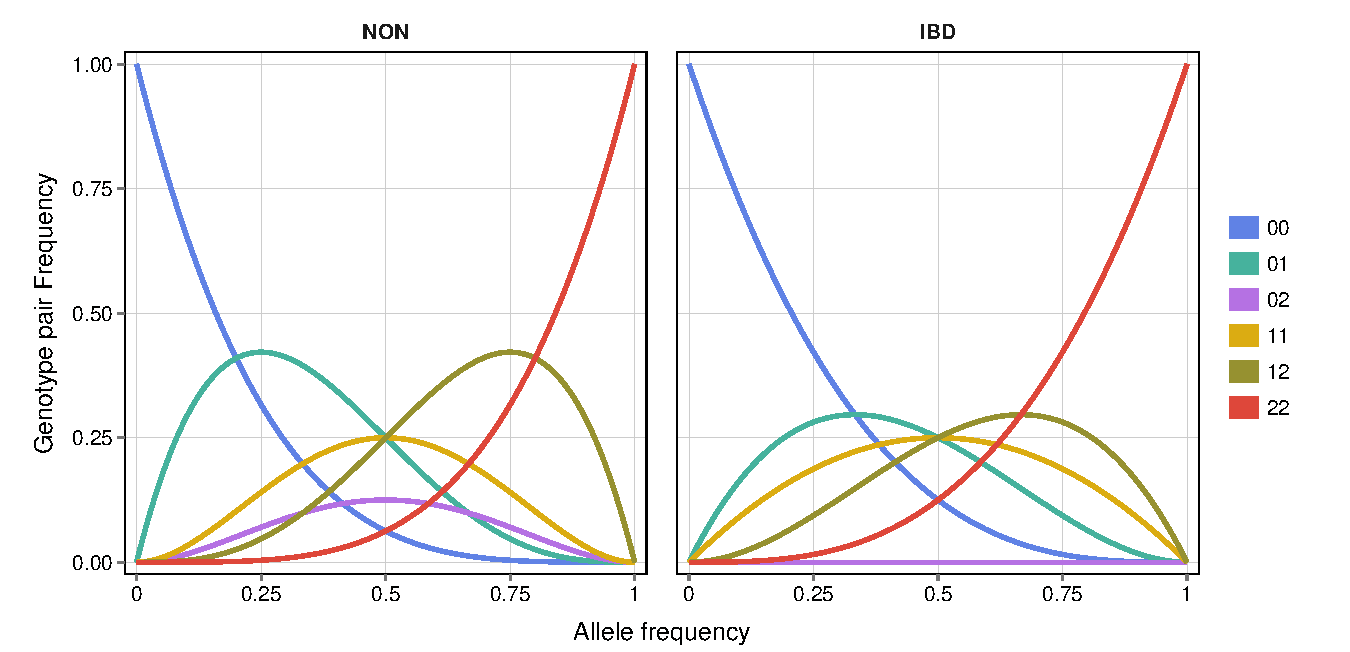
\includegraphics[width=\textwidth]{./img/ch4/exp-genpair-frq}
\Caption{Expected frequency distribution of genotype pairs under non-IBD and IBD}%
{Proportions were calculated using \cref{eq:genpairnon} and \cref{eq:genpairibd} in both hidden states, \emph{non} and \emph{ibd}, respectively.
Colours distinguish the \n{6} possible genotype pairs, given by $g_{k_1,k_2}$, as indicated.}%
{fig:exp_genpair_frq}
\end{figure}

%



%
% Replaced by above (simplified)
%
% First, the \emph{non} state is considered.
% Then, the formulations are extended to derive expectations in the \emph{ibd} state.
%
% \paragraph{Emission probabilities in the \emph{non} state.}
% Consider $m=2$ genotypes observed in a pair of individuals at a single locus.
% Each genotype can be observed in one of \n{3} possible states, which are again indexed by ${k \in \lbrace 0,1,2 \rbrace}$, where $k$ counts the alternate alleles that compose a genotype.
% Similarly, let $\alpha_{k}$ count the genotypes, $g_{k}$, that compose a genotype pair, ${g_{k_{1} k_{2}}}$.
% For example, the pair ${g_{0 0}}$ carries \n{2} $g_0$ genotypes, such that ${\alpha_{0} = 2}$, ${\alpha_{1} = 0}$, and ${\alpha_{2} = 0}$, the pair ${g_{0 1}}$ carries \n{1} $g_0$ and \n{1} $g_1$ genotype, such that ${\alpha_{0} = 1}$, ${\alpha_{1} = 1}$, and ${\alpha_{2} = 0}$, and so on.
% Expected pairwise frequencies follow a multinomial distribution.
% Recall that ${f_{g}(k) = {{n}\choose{k}}~p^{n-k}~q^{k}}$ where ${n=2}$, as given in \ctref{eq:genpropk}.
% In the general case, that is in a randomly mating population, genotypes in both individuals are assumed to be independent.
% It follows that the expected frequency of a given genotype pair is the joint probability of the expected genotype frequencies involved; expressed below.
% \begin{equation}\label{eq:genpairalpha}
% 	f_\textit{pair}(\alpha_{0}, \alpha_{1}, \alpha_{2}) = {{m}\choose{\alpha_{0}, \alpha_{1}, \alpha_{2}}}~\prod_{k=0}^{m} f_{g}(k)^{\alpha_{k}}
% \end{equation}
% The order of genotypes in a pair is ignored; \eg the pairs ${g_{01}}$ and ${g_{10}}$ are identical.
% In the following, the order ${k_1 \leq k_2}$ is preferred in notation.
% Note that the expected frequency for a pair of diploid genotypes cannot be represented by assuming a ploidy level of ${n=4}$ in \cref{eq:genpropk}.
% For example, the frequency of genotype pair ${g_{02}}$ is different to the frequency of ${g_{11}}$, despite the same number of allelic types that compose the genotypes in the pair, but which would be equal if \cref{eq:genpropk} is used.
% It is therefore necessary to distinguish genotypes by individual.
%
% The probability of observing a given genotype pair in \emph{non} can now be modelled using \cref{eq:genpairalpha}.
% However, for convenience, the following function is used, which dependents only on $k_1$~and~$k_2$;
% \begin{equation}\label{eq:genpairnon}\onehalfspacing
% 	\eta_{k_1 k_2} ~=~
%   \begin{cases}
% 		~ p^4       & ~ \text{if $k_1 = 0$, ~ $k_2 = 0$} \\
%     ~ 4 p^3 q   & ~ \text{if $k_1 = 0$, ~ $k_2 = 1$} \\
%     ~ 2 p^2 q^2 & ~ \text{if $k_1 = 0$, ~ $k_2 = 2$} \\
%     ~ 4 p^2 q^2 & ~ \text{if $k_1 = 1$, ~ $k_2 = 1$} \\
%     ~ 4 p q^3   & ~ \text{if $k_1 = 1$, ~ $k_2 = 2$} \\
%     ~ q^4       & ~ \text{if $k_1 = 2$, ~ $k_2 = 2$}
%   \end{cases}
% \end{equation}
% where $p$ and ${q=1-p}$ correspond to the frequency of the reference and alternate allele, respectively, in the sample at the current site in the sequence.
%
%
% \paragraph{Emission probabilities in the \emph{ibd} state.}
% The formulations derived in the previous paragraph assume a pair of unrelated individuals; that is if alleles are independently distributed in the population and haplotype occurrence in individuals is random.
% This assumption does not hold if the \n{2} individuals share a haplotype identical by descent.
% Because it is not straightforward to arrive at a similarly simple expression as given in \cref{eq:genpairalpha}, it is more convenient to construct a function similar to \cref{eq:genpairnon}.
% For this purpose see \cpref{tab:genpairprop}, which provides a more intuitive representation of the composition of haplotypes in each genotype pair, where the allelic contribution in each pair is illustrated for both \emph{non} and \emph{ibd}.
%
% If a haplotype is shared by both individuals, some combinations of alleles cannot be observed under \emph{ibd}; see \cref{tab:genpairprop}{b}.
% For example, if individual~1 carries the genotype $g_0$ and individual~2 carries $g_2$ at a given site in the sequence, the observation of the genotype pair $g_{02}$ has zero probability in \emph{ibd}, as the possibility to share a haplotype is precluded.
% The probability of any given genotype pair in \emph{ibd} can be expressed using the function below.
% \begin{equation}\label{eq:genpairibd}\onehalfspacing
% 	\delta_{k_1 k_2} ~=~
%   \begin{cases}
% 		~ p^3           & ~ \text{if $k_1 = 0$, ~ $k_2 = 0$} \\
%     ~ 2 p^2 q       & ~ \text{if $k_1 = 0$, ~ $k_2 = 1$} \\
%     ~ 0             & ~ \text{if $k_1 = 0$, ~ $k_2 = 2$} \\
%     ~ p^2 q + p q^2 & ~ \text{if $k_1 = 1$, ~ $k_2 = 1$} \\
%     ~ 2 p q^2       & ~ \text{if $k_1 = 1$, ~ $k_2 = 2$} \\
%     ~ q^3           & ~ \text{if $k_1 = 2$, ~ $k_2 = 2$}
%   \end{cases}
% \end{equation}
%



%
\subsubsection{Initial state probabilities}
\label{sec:HmmInit}
%

The model parameter $\pi$ stores the probabilities of being in either state at the start of the sequence.
Since the focal allele is used to identify the shared haplotype in a pair of individuals, the probability of being in \emph{ibd} is assumed to be ${\pi_\textit{ibd} = 1}$, such that ${\pi_\textit{non} = 0}$.




%
\subsection{Integration of empirically determined error rates}
\label{sec:HMMError}
%

In this section, the data generated in \cpref{sec:generrprofiles} were used to inform the model parameters in the \gls{hmm}.
This was done, first, to validate the expectations formulated in the previous sections, second, to explore variation instigated by genotype error and, third, to obtain empirical parameter values for emission and initial state probabilities in \emph{non} and \emph{ibd}.

Note that the effect of genotype error on state transition probabilities is not considered.
The computation of transition probabilities include the expected age of a focal allele dependent on its frequency, which could be biased in presence of genotype error, but where deviations are expected to be negligibly small if sample size is large.
In particular, the expected age represents an approximation to the \gls{tmrca} of the focal allele, which is more likely to be affected by unconsidered demographic parameters such as selection, migration, growth, and population structure, as well as sampling bias.

\N{2} datasets were available from previous analyses; the original genotype matrix as produced from simulated haplotypes, denoted by $\mathcal{D}$, and a corresponding, but modified genotype matrix, $\mathcal{D}^\ast$, in which the empirical, frequency-dependent proportions of genotype error were included in \cpref{sec:impact_error_data}.
These datasets allowed analysis \emph{before} and \emph{after} error, respectively.
Data consisted of ${n = \num{2500}}$ individuals and ${m = \num{672847}}$ variant sites.


%
\subsubsection{Empirical emission probabilities}
%

Information about IBD status was available through coalescent records obtained in the simulation.
By performing scans over all coalescent trees, true IBD intervals were determined for \fk{} variants at ${k \in \lbrace 2, \ldots, 25 \rbrace}$ (allele frequency between 0.04\% and 0.5\%).
In total, a set of \dec{11.597968}~million true IBD segments was compiled.
Each segment was recorded as a tuple of \n{2} breakpoint coordinates ($b_L$ and $b_R$ to the left and right-hand side of a focal variant, respectively) and \n{2} individuals, \ie indices for the pair of individuals who share a haplotype identical by descent within the breakpoint interval.

The set of compiled IBD segments was used to determine the empirical probability to observe a given genotype pair in \emph{ibd}.
This was done by randomly sampling \n{500000} segments with replacement, for which genotype data were extracted in ${[b_{L+1}, b_{R-1}]}$ for the \n{2} individuals.
Note that breakpoint sites were excluded to ensure IBD over the entire region.
For each segment, extracted genotype sequences were paired and collected by their coordinates along the length of the chromosome.
In a similar fashion, the empirical probability of observing genotype pairs in \emph{non} was determined using the same sample of segments, but where the \n{2} individuals sharing the IBD segment were ignored.
Instead, the \n{2} individuals were drawn at random from the subset of samples which did not share a haplotype IBD within ${[b_{L+1}, b_{R-1}]}$.
After sampling was complete, genotype pairs were aggregated by allele frequency per site, such that the frequency-dependent proportion of each genotype pair could be calculated in \emph{ibd} and \emph{non}.
In both cases, genotype data were taken separately from $\mathcal{D}$ and $\mathcal{D}^\ast$ to measure proportions before and after error.

%
% !TEX root = ../../main.tex


\begin{figure}[p]
{\scriptsize \texthv{\textbf{(a)} Before genotype error}} \\
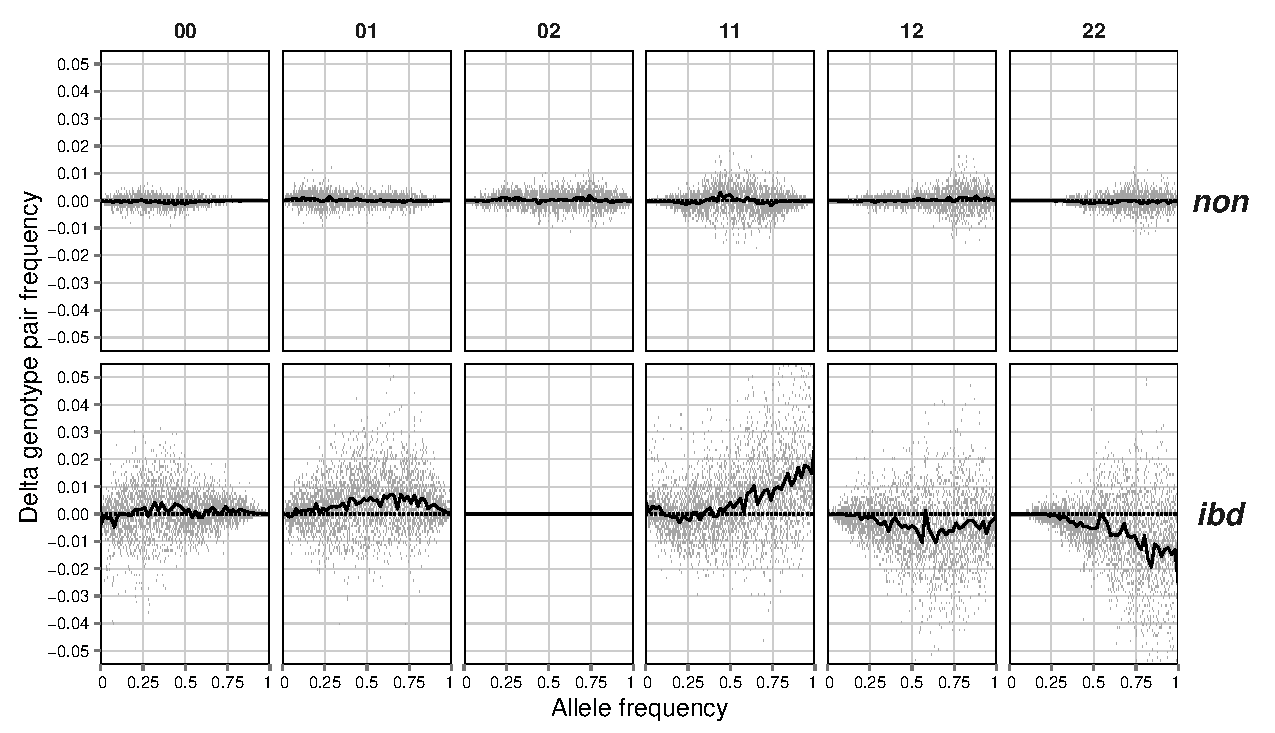
\includegraphics[width=\textwidth]{./img/ch4/hmm_emission_delta_tru}
{\scriptsize \texthv{\textbf{(b)} After genotype error}} \\
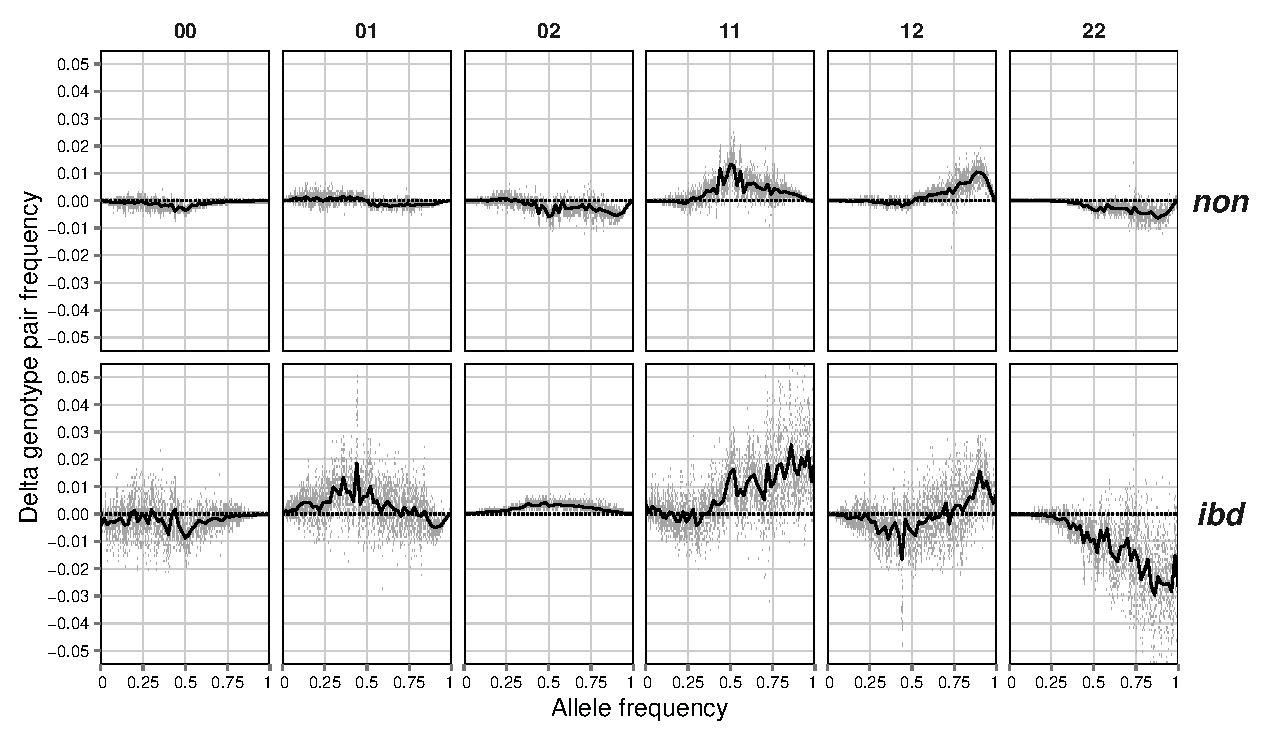
\includegraphics[width=\textwidth]{./img/ch4/hmm_emission_delta_err}
\Caption{Difference between empirical and expected proportions of genotype pairs}
{In total, \n{500000} segments were sampled in \emph{non} and \emph{ibd} as determined from coalescent records.
Segments were aggregated by allele frequency to calculate empirical proportions for each of the \n{6} possible genotype pairs (${g_{k_1,k_2}}$, indicated above each panel).
Delta values were calculated by subtracting empirical from expected proportions; the latter were calculated using \cref{eq:genpairnon,eq:genpairibd} under \emph{non} and \emph{ibd}, respectively.
Each panel is a scatterplot showing the deviation at each discrete step in allele frequency.
The mean (${\pm\text{SE}}$) of delta values was calculated in steps of 1\% allele frequency; indicated by the \emph{black} line.
Results in Panel~\textbf{(a)} were generated on data before the inclusion of genotype error, $D$, and Panel~\textbf{(b)} on data after genotype error was included, $D^{\ast}$.}
{fig:hmm_emission_delta}
\end{figure}

%

The resulting probability distributions after error were used to define the empirical emission model in \emph{ibd} and \emph{non}, again denoted by $\delta_{k_1 k_2}$ and $\eta_{k_1 k_2}$, respectively.
For illustration, deviations from expected genotype pair proportions are shown in \cpref{fig:hmm_emission_delta}, both before error (\ref{fig:hmm_emission_delta}{a}) and after error (\ref{fig:hmm_emission_delta}{b}).
Expectations in \emph{ibd} and \emph{non} were calculated according to \ctref{eq:genpairnon,eq:genpairibd}, respectively.
Differences were calculated by subtracting empirical from expected genotype pair proportions, which was done in discrete allele frequency units, but also averaged per frequency bin, in \n{100} bins of equal size across the allele frequency spectrum.

Before error, empirical and expected proportions in \emph{non} were equal on average, in each of the \n{6} possible genotype pairs.
The variability along the allele frequency spectrum was negligibly small, where deviations per frequency unit were seen as stochastic noise around the mean and ranged between $-1\%$~and~$+1\%$.
In contrast, the variability across frequency units was overall amplified in \emph{ibd}.
The mean proportion of $g_{11}$ was up to 2\% higher than expected towards the higher end of the frequency spectrum, whereas $g_{22}$ was up to 2\% lower than expected towards higher frequencies.
Notably, $g_{02}$ is expected to have a constant zero probability of observation in \emph{ibd}, which was confirmed from the data.
% However, a few sites were found where $g_{02}$ was observed at non-zero probabilities in \emph{ibd}.
% Upon inspection, these were found to correspond to sites where multiple IBD segments shared by the same \n{2} individuals overlapped, such that the segments were underestimated.

After error, overall variability increased in each comparison.
In \emph{non}, the mean proportion of $g_{11}$ showed deviations of up to $+1\%$ towards 50\% allele frequency, which was also seen for $g_{12}$, but towards higher frequencies.
In \emph{ibd}, mean proportions showed as similar distribution as in comparisons before error, but where the difference between empirical and expected values was further increased.
For example, deviations of $g_{11}$ were increased up to $+2.5\%$ towards higher frequencies, which was mirrored by $g_{22}$ but reaching up to $-3\%$.
Importantly, on average the empirical proportion of $g_{02}$ was non-zero along the frequency spectrum, but which increased up to $+0.5\%$ towards 50\% allele frequency.


%
\subsubsection{Empirical initial state probabilities}
%

Genotype error can affect the allele frequency distribution and thus bias the identification of individuals which share an allele at a given site.
Some of the formed pairs may therefore be wrongly included, whereas some others may be missed.
In particular, the following \n{4} cases can be distinguished:
\begin{case}
	\item\label{case:true_pos} \textbf{True~positives.} The focal allele correctly identifies haplotype sharing in \n{2} individuals which are heterozygous for the allele; \ie ${g_{1} \rightarrow g_{1}}$.
	\item\label{case:false_pos} \textbf{False~positives.} The focal allele is observed in a misclassified genotype, ${g_{0} \rightarrow g_{1}}$, such that IBD is wrongly assumed for a pair which does not share a haplotype.
	Note that the change ${g_{2} \rightarrow g_{1}}$ also leads to the inclusion of an individual which actually is homozygous for the focal allele, but which is not considered in the model.
	\item\label{case:false_neg} \textbf{False~negatives.} The genotype of an individual was misclassified at the focal site, ${g_{1} \rightarrow g_{0}}$, such that the focal allele is missed and the individual wrongly excluded.
	Note that this also considers the change ${g_{1} \rightarrow g_{2}}$, leading to the exclusion of the individual due to the assumptions of the model.
	\item\label{case:true_neg} \textbf{True~negatives.} An individual is correctly excluded due to not being heterozygous for the focal allele, \ie ${g_{0} \rightarrow g_{0}}$ or ${g_{2} \rightarrow g_{2}}$, as well as ${g_{0} \rightarrow g_{2}}$ or ${g_{2} \rightarrow g_{0}}$
\end{case}

The inference of IBD segments in a pair where at least \n{1} individual is a false positive, \cref{case:false_pos}, is likely to result in a disproportionately reduced segment length.
In principle, such falsely identified individuals, and thereby specific false genotypes, may be exposed if segment lengths are consistently shorter than expected in each pairwise analysis.
On the other hand, genotype error leading to false negatives, \cref{case:false_neg}, is inadvertently missed, because it is not directly possible to assume that particular individuals carry the focal allele if not observed in the data.

The proportion of genotype pairs identified as true positives, \cref{case:true_pos}, is relevant to determine the probability of the initial state at the start of the sequence.
The true positive rate was determined by comparison of the data before and after error.
All \fk{} variants at ${k > 1}$ were identified in $\mathcal{D}^\ast$, as well as all the individuals carrying the alternate allele at a particular variant site.
This resulted in a set of matrix coordinates (marker by individual) which were pooled into site frequency bins, defined by $k$.
Bins with less than \n{1000} markers were removed.
Then, for each $k$, all possible pairs of individuals were formed at each marker and the dataset $\mathcal{D}$ was queried with the joint set of coordinates.
This was done to extract the corresponding vector of true genotype pairs, from which the true positive rate was calculated as the proportion of pairs in which both genotypes were heterozygous.

%
% !TEX root = ../../main.tex


\begin{figure}[!htb]
\centering
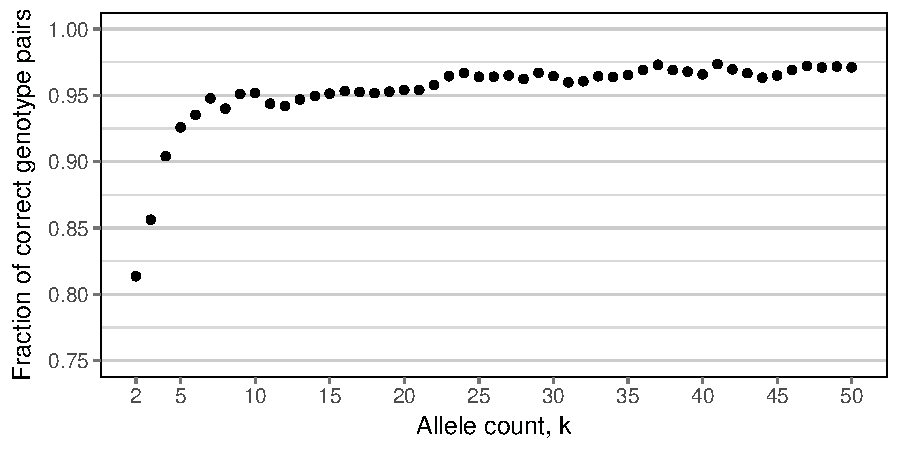
\includegraphics[width=0.9\textwidth]{./img/ch4/hmm_initial}
\Caption{True positive rate of identified genotype pairs at focal sites}
{Pairwise shared genotypes at focal \fk{} variants with $k > 1$ were compared between datasets before and after error.
The true positive rate was determined for each $k$.
Results are shown for $k$~in~${[2,50]}$, which corresponds to an allele frequency between 0.04\% and 1\%.}
{fig:hmm_initial}
% \vspace{-5pt}
% \hrulefill%
\end{figure}

%

The empirical distribution of correctly identified genotype pairs was used to define the initial state probability of being in \emph{ibd}, given the frequency of the focal allele expressed in \fk{}.
The resulting distribution is shown in \cpref{fig:hmm_initial}, for focal variants with $k$ in ${[2, 50]}$, corresponding to an allele frequency between 0.04\% and 1\%.
The fraction of correctly observed genotype pairs was lowest for \fk{2} variants, found at \dec{0.812}, but rapidly increased to \dec{0.913} and \dec{0.95} for \fk{5} and \fk{10} variants, respectively.
At higher frequencies, the true positive rate stabalised around \dec{0.975}~and~\dec{0.995}.
At frequencies near 100\%, however, the number of markers observed per $k$ was too low to provide conclusive estimates.
These values were stored in an array such that the initial state probability for a given $k$ can be accessed through the functions $\pi_\textit{ibd}(k)$ and ${\pi_\textit{non}(k) = 1 - \pi_\textit{ibd}(k)}$.



%
\subsection{Inference of IBD segments}
%

The aim of the presented IBD-model is to find the most likely position along the sequence at which the \emph{ibd} state changes into the \emph{non} state, which is done independently to the left and right-hand side of the focal \fk{}~variant; \ie the focal site sits at the start of both observation sequences.
Recall that the IBD segment around the focal variant is defined by the interval ${[b_L, b_R]}$, where $b_L$ and $b_R$ denote the breakpoints which delimit the region in which at least \n{1} recombination event is likely to have occurred to the left and right-hand side of the focal variant site at position $b_i$.
To infer this interval, the most likely hidden state which generated the observed genotype pair is inferred at each site along the sequence.
In general, given ${H}$ hidden states and an observation sequence of length~$m$, there are $H^m$ possible state sequences.
For example, given this \n{2}-state \gls{hmm} and a short region of only \n{100} genotype pairs, the number of possible state sequences already exceeds the number of seconds the universe has existed\footnote{Current age of the universe: \num{42e16} seconds \accessed{2017}{02}{18}}.
To circumvent this problem, \citet{Rabiner:1989hs} formally advised the use of the \emph{Viterbi~algorithm} for sequence classification in \glspl{hmm}, which scales quadratically with the number of hidden states and has a time complexity of ${O(H^2 m)}$.

%
% \subsubsection{Viterbi algorithm}
%

The Viterbi algorithm is a dynamic programming technique which finds the most likely sequence of hidden states that maximises the probability of observing the data \citep{Viterbi:1967hq,Forney:1973dt}.
Let $X_j$ denote the hidden state at site~$j$ which generated the observed genotype pair $o_j$.
Following \citet{Rabiner:1989hs}, the probability of the most likely sequence of hidden states until site~$j$ and ending in state~$x$ is given by
\begin{equation}\label{eq:viterbi_main}
	v_j(x) ~=~ \max_{X_0, X_1, \ldots, X_{j-1}} P(X_0, X_1, \ldots, X_{j-1},~ X_j = x,~ o_1, o_2, \ldots, o_j \mid \lambda)
\end{equation}
where $\lambda$ denotes the model; see \ctref{eq:hmm_model}.
% By induction, it follows that
% \begin{equation*}
% 	v_{j+1}(x)  & ~=~ \delta_j(o_j) ~ \max_{y \in S} \big[ v'_{j-1}(\textit{ibd}) ~ ~ \psi_{j,k}(y \mid \textit{ibd}) \big]
% \end{equation*}
The procedure to retrieve the actual state sequence is summarised as follows.

\begin{enumerate}[label=\textbf{\arabic*.},leftmargin=*]
	\item \textbf{Initialisation.} %
	% \begin{equation}
	% 	u_0(x) ~=~ 0 \quad \forall \quad x \in S
	% \end{equation}
	The probability that a given state generated the genotype pair observed at the focal site is simply the product of its initialisation and emission probabilities.
	If genotype error is included, the initialisation probability is defined conditionally on the frequency of the focal \fk{}~variant.
	Note that emission probabilities were defined as ${\delta_{k_1 k_2}}$ and ${\eta_{k_1 k_2}}$ in \emph{ibd} and \emph{non}, respectively.
	For simplicity, these are now written as ${\delta_j(o_j)}$ and ${\eta_j(o_j)}$, where the index~$j$ refers to the position in the sequence at which the allele frequency is taken to retrieve the frequency-dependent probability of the observed genotype pair at site~$j$.
	\begin{align}
	\begin{aligned}
		v_0(\textit{ibd}) & ~=~ \pi_\textit{ibd}(k) ~ \delta_0(o_0) \\
		v_0(\textit{non}) & ~=~ \pi_\textit{non}(k) ~ \eta_0(o_0)
	\end{aligned}
	\end{align}

	The Viterbi algorithm involves the successive multiplication of probabilities during the recursion step (see below), which may result in values too small to be distinguishable from \n{0} using conventional computers.
	To avoid this problem, a commonly implemented solution is a log-transformation of probabilities.
	Here, it is more convenient (and computationally less demanding) to define a weighting function to obtain a scaling factor which is stored in an additional array,~$w$.
	\begin{equation}
		w_0 ~=~ \max_{x \in S} \big[ v_0(x) \big] \quad\textbf{s.t.}\quad
		v'_0(x) ~=~ \frac{v_0(x)}{w_0} \quad \forall \quad x \in S
	\end{equation}

	\item \textbf{Recursion.} The array $u$ is defined to keep track of the states traversed along the path; that is, ${u_j(x)}$ stores a back-pointer to the state at site~$j-1$ which resulted in the highest probability ${v_j(x)}$ at site~$j$.
	\begin{equation}
		u_j(x) ~=~ \argmax_{y \in S} \big[ v'_{j-1}(x) ~ \psi_{j,k}(y \mid x) \big] \quad \forall \quad x \in S; ~ j = 1, 2, \ldots, m
	\end{equation}
	Recall that ${\psi_{j,k}}$ refers to the transition probability from a given state to another or the same state, and is dependent on the frequency of the focal allele ($k$), as defined in \ccref{eq:hmm_trans_prob}.
	The chain proceeds through the most likely path at each site along the sequence by following the transitions that maximise the probability of observing a given state.
	Given \cref{eq:viterbi_main}, by induction on $j$ it follows that
	\begin{align}
	\begin{aligned}
		v_j(\textit{ibd})  & ~=~ \delta_j(o_j) ~ \max_{y \in S} \big[ v'_{j-1}(\textit{ibd}) ~ ~ \psi_{j,k}(y \mid \textit{ibd}) \big]\ , & j = 1, 2, \ldots, m\phantom{.} \\
		v_j(\textit{non})  & ~=~ \eta_j(o_j) ~ \max_{y \in S} \big[ v'_{j-1}(\textit{non}) ~ \psi_{j,k}(y \mid \textit{non}) \big]\ , & j = 1, 2, \ldots, m.
	\end{aligned}
	\end{align}

	Note that the current state probability is computed conditionally on the weighted probability value at the immediate previous site, but which does not affect the outcome of the maximisation.
	\begin{equation}
		w_j ~=~ \max_{x \in S} \big[ v_j(x) \big] \quad\textbf{s.t.}\quad
		v'_j(x) ~=~ \frac{v_j(x)}{w_j} \quad \forall \quad x \in S; ~ j = 1, 2, \ldots, m
	\end{equation}

	\item \textbf{Termination.} At the last site in the sequence, $m$, the state with the highest probability is picked to mark the final state of the most likely sequence of hidden states (\ie the ``Viterbi path''), denoted by ${X^\ast}$.
	\begin{equation}
		X^\ast_m ~=~ \argmax_{x \in S} \big[ v'_{m}(x) \big]
	\end{equation}

	\item \textbf{Path backtracking.} Given the array of back-pointers, $u$, the most likely path is found by tracing back from the final state until the initial site in the sequence.
	\begin{equation}
		X^\ast_j ~=~ u_{j+1}\left(X^\ast_{j+1}\right)\ , \quad j = m-1, m-2, \ldots, 0
	\end{equation}
\end{enumerate}

The IBD segment is determined from the \n{2} resulting state sequences, which were obtained independently from the observation sequence to the left and right-hand side of the focal position.
The Viterbi paths on the left and right-hand side are denoted by $L^\ast$ and $R^\ast$, respectively.
The breakpoint interval defining the segment, ${[b_L, b_R]}$, is found by scanning each path from its start (\ie from a given target site) to the first position at which the \emph{non} state was inferred.
Note that this includes the site of the first \emph{non} state, which is defined as a breakpoint.
In boundary cases, when each site until the end of the chromosome was inferred as being in the \emph{ibd} state, the last site in the sequence is taken as a breakpoint.





%
\subsection{Results}
%


The \gls{hmm}-based method for IBD inference was evaluated on the same error-treated dataset as used in \cpref{sec:ibd_results_err}, as well as the corresponding dataset before the integration of (realistic) error rates.
\Addition{As was done in the previous analyses, if multiple identical breakpoint intervals were inferred for a given pair, only the one detected around the allele of the lowest frequency within that interval was retained (or one was sampled if multiple shared alleles occurred at the same frequency).
The retained (\emph{unique}) segments were thereby tagged by the presumably youngest shared allele within a given interval, such that breakpoint accuracy could be measured conditional on the frequency of the target allele.}


%
\subsubsection{Shared haplotype inference in simulated data before and after error}
%

The number of unique segments inferred was
\dec{3.179340}~million and
\dec{3.236198}~million before and after error, which corresponds to
\SI{32.25035}{\percent} and
\SI{32.82710}{\percent} of the reported set of IBD segments, respectively.
In comparison, the number of unique segments in the set of true IBD segments, those determined from simulation records on the same targets, was
\dec{2.720789}~million (\SI{27.59894}{\percent}).
The proportion of breakpoints overestimated \Addition{(relative to the corresponding true breakpoint position)} was similar \Correct{for} both datasets;
\SI{55.71575}{\percent} before error and
\SI{54.09442}{\percent} after error.

%
% !TEX root = ../../main.tex


\begin{table}[!htb]
\Caption{Accuracy comparison per $\textbf{f}_{k}$~category after error}
{The accuracy of detected IBD breakpoints was measured using the squared Pearson correlation coefficient, $r^2$, and the \gls{rmsle} in relation to the true IBD segments determined from simulation records; measured in terms of the distance between breakpoint site and the corresponding focal position per segment.
Results were obtained on the error-treated dataset, $D^\ast$ (which included the true haplotypes, phased haplotypes, and genotype data), using the \gls{fgt}, \gls{dgt}, and the \gls{hmm}-based method for targeted IBD detection.
Accuracy was measured after duplicate segments had been removed, and the same set of target sites was assessed in each approach; separately computed per \fk{}~category.
The approach with the highest accuracy (highest $r^2$ and lowest \gls{rmsle}) per \fk{} is indicated (\textbf{bold}).}
{tab:stat_hmm_accuracy}
\centering
\begin{threeparttable}
\begin{tabular}{cc*8{S[table-format=1.3]}}
\toprule
\fk{} & Freq.~(\%) &
\multicolumn{4}{c}{$r^2$} &
\multicolumn{4}{c}{$\rmsle$} \\
\cmidrule(lr){3-6}
\cmidrule(lr){7-10}
 & &
 \multicolumn{1}{c}{\textsc{fgt}$^{\ast}$} &
 \multicolumn{1}{c}{\textsc{fgt}$^{\ast\ast}$} &
 \multicolumn{1}{c}{\textsc{dgt}} &
 \multicolumn{1}{c}{\textsc{hmm}} &
 \multicolumn{1}{c}{\textsc{fgt}$^{\ast}$} &
 \multicolumn{1}{c}{\textsc{fgt}$^{\ast\ast}$} &
 \multicolumn{1}{c}{\textsc{dgt}} &
 \multicolumn{1}{c}{\textsc{hmm}} \\
\midrule
2  & 0.04  &  0.010582 & 0.014582 & 0.018248 & \bfseries 0.98195  &  1.20751 & 1.36188 & 1.02893 & \bfseries 0.39000 \\
3  & 0.06  &  0.031067 & 0.038874 & 0.050454 & \bfseries 0.90796  &  1.01260 & 1.11170 & 0.85521 & \bfseries 0.45189 \\
4  & 0.08  &  0.049067 & 0.060465 & 0.079352 & \bfseries 0.83170  &  0.92372 & 0.99300 & 0.79179 & \bfseries 0.48982 \\
5  & 0.10  &  0.064336 & 0.074557 & 0.097068 & \bfseries 0.75534  &  0.86949 & 0.91291 & 0.75632 & \bfseries 0.53408 \\
6  & 0.12  &  0.084372 & 0.092725 & 0.119511 & \bfseries 0.68236  &  0.83166 & 0.86309 & 0.72973 & \bfseries 0.55506 \\
7  & 0.14  &  0.088915 & 0.096974 & 0.122594 & \bfseries 0.60158  &  0.79130 & 0.80977 & 0.71099 & \bfseries 0.58238 \\
8  & 0.16  &  0.093825 & 0.105791 & 0.134537 & \bfseries 0.57518  &  0.76712 & 0.78372 & 0.69163 & \bfseries 0.58823 \\
9  & 0.18  &  0.104740 & 0.112222 & 0.137905 & \bfseries 0.52273  &  0.75373 & 0.76617 & 0.69034 & \bfseries 0.61330 \\
10 & 0.20  &  0.112664 & 0.123376 & 0.147052 & \bfseries 0.49230  &  0.73296 & 0.74033 & 0.68234 & \bfseries 0.63476 \\
11 & 0.22  &  0.121881 & 0.128264 & 0.148674 & \bfseries 0.44025  &  0.71292 & 0.71555 & 0.67724 & \bfseries 0.65865 \\
12 & 0.24  &  0.139354 & 0.144022 & 0.173480 & \bfseries 0.42443  &  0.71754 & 0.72058 & 0.69105 & \bfseries 0.65362 \\
13 & 0.26  &  0.117257 & 0.119571 & 0.153604 & \bfseries 0.42399  &  0.70820 & 0.71069 & 0.68634 & \bfseries 0.67524 \\
14 & 0.28  &  0.149290 & 0.157222 & 0.177873 & \bfseries 0.38611  &  0.69893 & 0.69564 & 0.68322 & \bfseries 0.67801 \\
15 & 0.30  &  0.126124 & 0.129022 & 0.150514 & \bfseries 0.40773  &  0.69136 & 0.69047 & \bfseries 0.67632 & 0.68097 \\
16 & 0.32  &  0.146263 & 0.150035 & 0.175060 & \bfseries 0.37855  &  0.67615 & 0.67513 & \bfseries 0.66921 & 0.68919 \\
17 & 0.34  &  0.132252 & 0.139972 & 0.158276 & \bfseries 0.31246  &  0.68322 & \bfseries 0.68194 & 0.69011 & 0.71230 \\
18 & 0.36  &  0.142659 & 0.157670 & 0.175474 & \bfseries 0.33410  &  0.66938 & \bfseries 0.66725 & 0.66936 & 0.70196 \\
19 & 0.38  &  0.149018 & 0.153322 & 0.169780 & \bfseries 0.30284  &  0.67484 & \bfseries 0.66858 & 0.67281 & 0.70459 \\
20 & 0.40  &  0.172848 & 0.178531 & 0.191955 & \bfseries 0.32734  &  0.66420 & \bfseries 0.66490 & 0.68145 & 0.71564 \\
21 & 0.42  &  0.154459 & 0.164816 & 0.172428 & \bfseries 0.30891  &  0.66722 & \bfseries 0.65987 & 0.68200 & 0.71979 \\
22 & 0.44  &  0.150849 & 0.154348 & 0.160300 & \bfseries 0.25738  &  0.65879 & \bfseries 0.65733 & 0.68402 & 0.72529 \\
23 & 0.46  &  0.139355 & 0.143699 & 0.160249 & \bfseries 0.26530  &  0.65271 & \bfseries 0.64871 & 0.67536 & 0.72320 \\
24 & 0.48  &  0.152718 & 0.152657 & 0.168426 & \bfseries 0.24662  &  0.66336 & \bfseries 0.65544 & 0.69046 & 0.74639 \\
25 & 0.50  &  0.097909 & 0.102016 & 0.102042 & \bfseries 0.23875  &  0.66417 & \bfseries 0.65579 & 0.70157 & 0.74032 \\
\bottomrule
\end{tabular}
\begin{tablenotes}\footnotesize
	\item[$\ast$] ~ True haplotypes
	\item[$\ast\ast$] ~ Phased haplotypes
\end{tablenotes}
\end{threeparttable}
\end{table}







% HMM, before & after error
% 2  & 0.04  &  0.98254 & 0.98195  &  0.38777 & 0.39000 \\
% 3  & 0.06  &  0.90867 & 0.90796  &  0.45110 & 0.45189 \\
% 4  & 0.08  &  0.83002 & 0.83170  &  0.48923 & 0.48982 \\
% 5  & 0.10  &  0.75737 & 0.75534  &  0.52929 & 0.53408 \\
% 6  & 0.12  &  0.67923 & 0.68236  &  0.55171 & 0.55506 \\
% 7  & 0.14  &  0.60472 & 0.60158  &  0.57820 & 0.58238 \\
% 8  & 0.16  &  0.57644 & 0.57518  &  0.58612 & 0.58823 \\
% 9  & 0.18  &  0.52700 & 0.52273  &  0.61032 & 0.61330 \\
% 10 & 0.20  &  0.49189 & 0.49230  &  0.63207 & 0.63476 \\
% 11 & 0.22  &  0.43732 & 0.44025  &  0.65599 & 0.65865 \\
% 12 & 0.24  &  0.43023 & 0.42443  &  0.65214 & 0.65362 \\
% 13 & 0.26  &  0.42761 & 0.42399  &  0.67293 & 0.67524 \\
% 14 & 0.28  &  0.38975 & 0.38611  &  0.67429 & 0.67801 \\
% 15 & 0.30  &  0.40691 & 0.40773  &  0.67814 & 0.68097 \\
% 16 & 0.32  &  0.38277 & 0.37855  &  0.68598 & 0.68919 \\
% 17 & 0.34  &  0.31571 & 0.31246  &  0.71091 & 0.71230 \\
% 18 & 0.36  &  0.33718 & 0.33410  &  0.69922 & 0.70196 \\
% 19 & 0.38  &  0.31051 & 0.30284  &  0.70173 & 0.70459 \\
% 20 & 0.40  &  0.33336 & 0.32734  &  0.71393 & 0.71564 \\
% 21 & 0.42  &  0.30974 & 0.30891  &  0.71842 & 0.71979 \\
% 22 & 0.44  &  0.26250 & 0.25738  &  0.72426 & 0.72529 \\
% 23 & 0.46  &  0.27133 & 0.26530  &  0.72038 & 0.72320 \\
% 24 & 0.48  &  0.24439 & 0.24662  &  0.74661 & 0.74639 \\
% 25 & 0.50  &  0.23466 & 0.23875  &  0.73934 & 0.74032 \\

%

Overall accuracy, \Addition{measured as the physical distance between breakpoint and target site,} was
${r^2=\dec{0.6340087}}$ (${\rmsle=\dec{0.7812424}}$) before error and
${r^2=\dec{0.6381827}}$ (${\rmsle=\dec{0.7911286}}$) after error.
While it appears from these results that accuracy was relatively low, consider accuracy measured per focal allele frequency.
\Cpref{tab:stat_hmm_accuracy} shows $r^2$ and $\rmsle$ measured per \fk{}~category, where the \gls{hmm} is compared to corresponding results obtained on the same set of target sites using the \gls{fgt} on true (simulated) haplotypes as well as phased haplotypes, and the \gls{dgt} on genotype data; \Addition{shown for analyses conducted after the integration of error.}
The HMM-based IBD detection approach outperformed each of the rule-based methods (in terms of $r^2$).
However, for each method, accuracy decreases rapidly towards higher frequencies.

%
% !TEX root = ../../main.tex


\begin{figure}[!htbp]
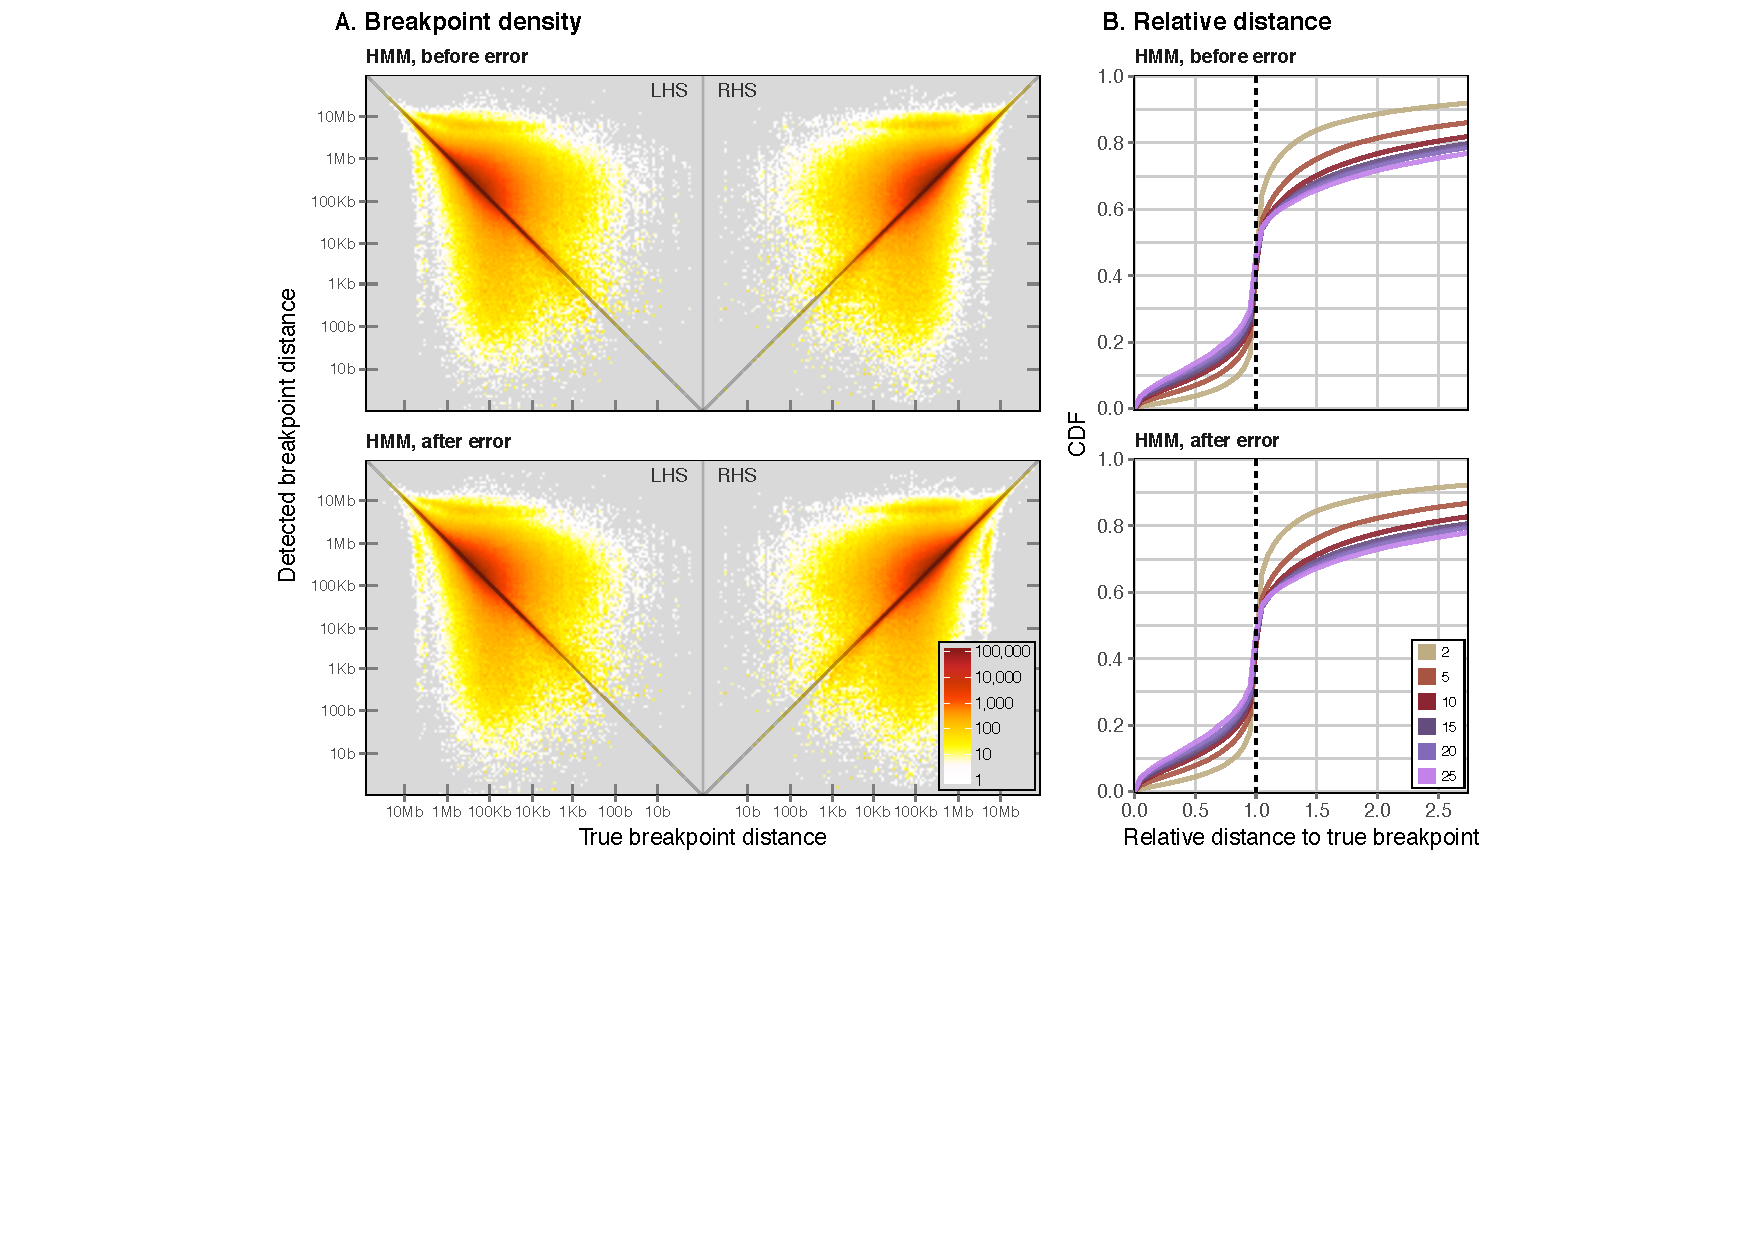
\includegraphics[width=\textwidth]{./img/ch4/break_hmm}
\Caption{Accuracy of IBD breakpoint detection using the Hidden Markov Model on simulated data, before and after error}
{Panel~\textbf{(A)} shows the density of true and detected breakpoints; Panel~\textbf{(B)} shows the physical length in terms of the relative distance between a focal site and the detected breakpoint.
See \cpref{fig:naive_break_err} for a detailed description.}
{fig:break_hmm}
\end{figure}

%

Median length was assessed after removal of boundary cases;
\SI{1.24133}{\percent} of segments were removed in the analysis conducted on data before the integration of error and \SI{1.21611}{\percent} after error.
This proportion was similar for the set of true IBD segments (\SI{1.37743}{\percent}).
Before error, overall median length was
\SI{0.525714}{\mega\basepair} (\SI{0.8837688}{\centi\morgan}), and
\SI{0.503856}{\mega\basepair} (\Correct{{\SI{0.8450367}{\centi\morgan}}}) after error; this is compared to the shorter median length found for the true dataset;
\SI{0.343451}{\mega\basepair} (\SI{0.5903069}{\centi\morgan}).
\Addition{At \fk{2} alleles, median length was
{\SI{2.208884}{\mega\basepair}} ({\SI{3.690252}{\centi\morgan}}) for the set of true shared haplotype segments, which is shorter compared to the inferred length of
{\SI{2.498538}{\mega\basepair}} ({\SI{4.207228}{\centi\morgan}}) before error and
{\SI{2.458135}{\mega\basepair}} ({\SI{4.129179}{\centi\morgan}}) after error.
Lengths decreased towards higher focal allele frequencies, but where inferred lengths still remained overestimated; \eg at \fk{25} alleles, median length for true segments was
{\SI{0.230837}{\mega\basepair}} ({\SI{0.406926}{\centi\morgan}}), compared to
{\SI{0.378793}{\mega\basepair}} ({\SI{0.626378}{\centi\morgan}}) before error and
{\SI{0.360072}{\mega\basepair}} ({\SI{0.593404}{\centi\morgan}}) after error.}
The distribution of IBD length by focal allele frequency is shown in \cpref{fig:length_hmm}\Delete{, which for comparison also includes the results obtained for the FGT and DGT after error}.


%
% !TEX root = ../../main.tex


\begin{figure}[!htb]
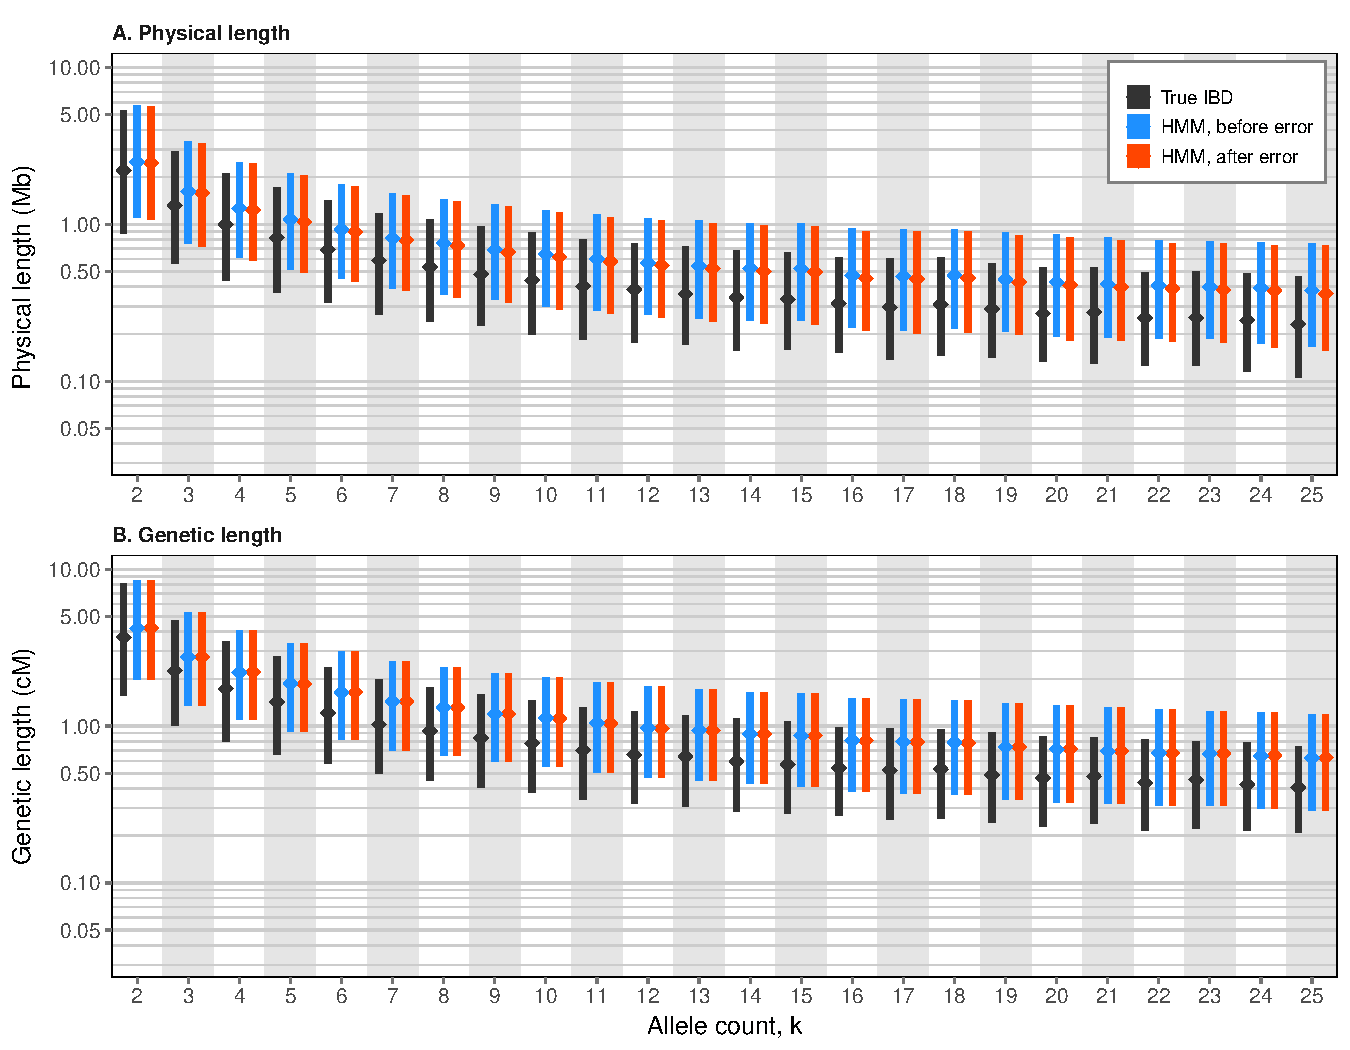
\includegraphics[width=\textwidth]{./img/ch4/length_hmm}
\Caption{IBD lengths using the HMM before and after error}
{The HMM-based approach for targeted IBD detection was applied to simulated data before and after the integration of error; \ie datasets $D$ and $D^\ast$, respectively.
Lengths were compared to the corresponding set of true breakpoint segments as determined from simulation records.
Bottom and top of each bar indicate \nth{1} and \nth{3} quartiles, respectively, between which the median (\nth{2} quartile) is marked (\emph{diamonds}).}
{fig:length_hmm}
\end{figure}

%



%
\subsubsection{Analysis of 1000 Genomes data, chromosome 20}
%

\AdditionNote{This section was re-written and extended to include additional results}

In the previous analysis of \gls{1kg} data in \cpref{sec:fgt_dgt_1kg20}, I showed that neither the \gls{fgt} nor the \gls{dgt} were likely to detect shared haplotype segments with sufficient accuracy.
I therefore attempted to demonstrate in this chapter (\cref{sec:impact_error_data}) that presence of error in the data can have a dramatic impact on such rule-based detection methods.
It was suggested that even relatively small error rates (as expected in real data) may lead to the detection of false positive breakpoints and, thus, the observation of truncated breakpoint intervals in the majority of scans.
In the section above, I demonstrated that the HMM-based approach for targeted shared haplotype inference is robust towards error, but where overall length of detected segments is likely to be overestimated.
Nonetheless, it should be possible to re-produce similar patterns when applying this method to real data.

%
% !TEX root = ../../main.tex


\begin{figure}[!htb]
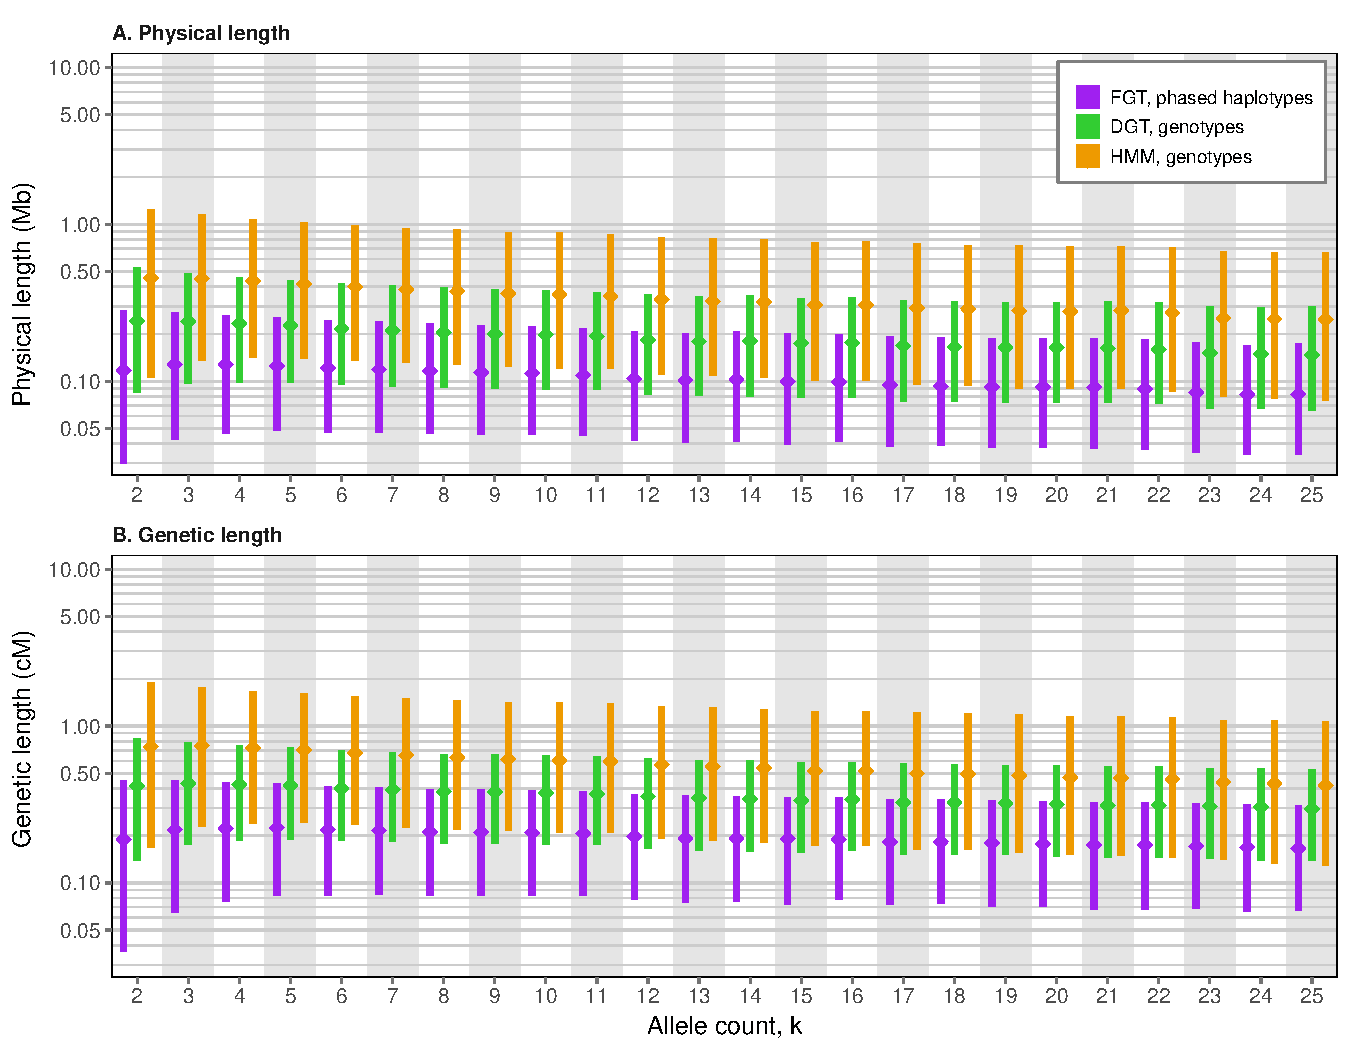
\includegraphics[width=\textwidth]{./img/ch4/1KG_chr20_length_hmm}
\Caption{IBD inference using the HMM on 1000 Genomes data, chr.~20}
{IBD detection using the HMM-based method was performed under the empirical error model defined on genotype data from the \glsentrylong{1kg}.
The resulting length distribution is compared to previous results obtained on the same set of target sites using the \gls{fgt} and \gls{dgt}.
Bottom and top of each bar indicate \nth{1} and \nth{3} quartiles, respectively, between which the median (\nth{2} quartile) is marked (\emph{diamonds}).}
{fig:1KG_chr20_length_hmm}
\end{figure}

%

I applied the HMM-based method to data from chromosome~20 in \glsentrylong{1kg} Phase~\rom{3} and inferred {\dec{18.040053}}~million shared haplotype segments around all variants observed at \fk{[2,25]} (\ie frequency below 0.5\%) of which {\Percent{39.32543}} were unique.
For direct comparison to corresponding results obtained using the \gls{fgt} and \gls{dgt} (see \cref{sec:fgt_dgt_1kg20}), I retained a random subset of 1~million unique segments that were inferred around the same target site and haplotype pair in each method, after also removing boundary cases.

Overall median physical (genetic) length was
\SI{0.311748}{\mega\basepair} (\SI{0.5383650}{\centi\morgan}) for the HMM-based detection method, which was longer compared to the \gls{fgt} and \gls{dgt} where median length was
\SI{0.097541}{\mega\basepair} (\SI{0.1897540}{\centi\morgan}) and
\SI{0.176087}{\mega\basepair} (\SI{0.3444909}{\centi\morgan}), respectively.
The distribution of IBD length by focal allele frequency is shown in \cpref{fig:1KG_chr20_length_hmm}.
While it is shown that only the HMM is able to infer longer IBD segments that are more consistent with expectations, such a comparison is limited due to population structure in the \gls{1kg} sample.
For example, the simulated dataset was generated as a sample of ``European'' haplotypes only (as defined in the demographic model; see \ccref{sec:sim_demo_model}.

%
% !TEX root = ../../main.tex


\begin{figure}[p]
\centering
\makebox[\textwidth][c]{%
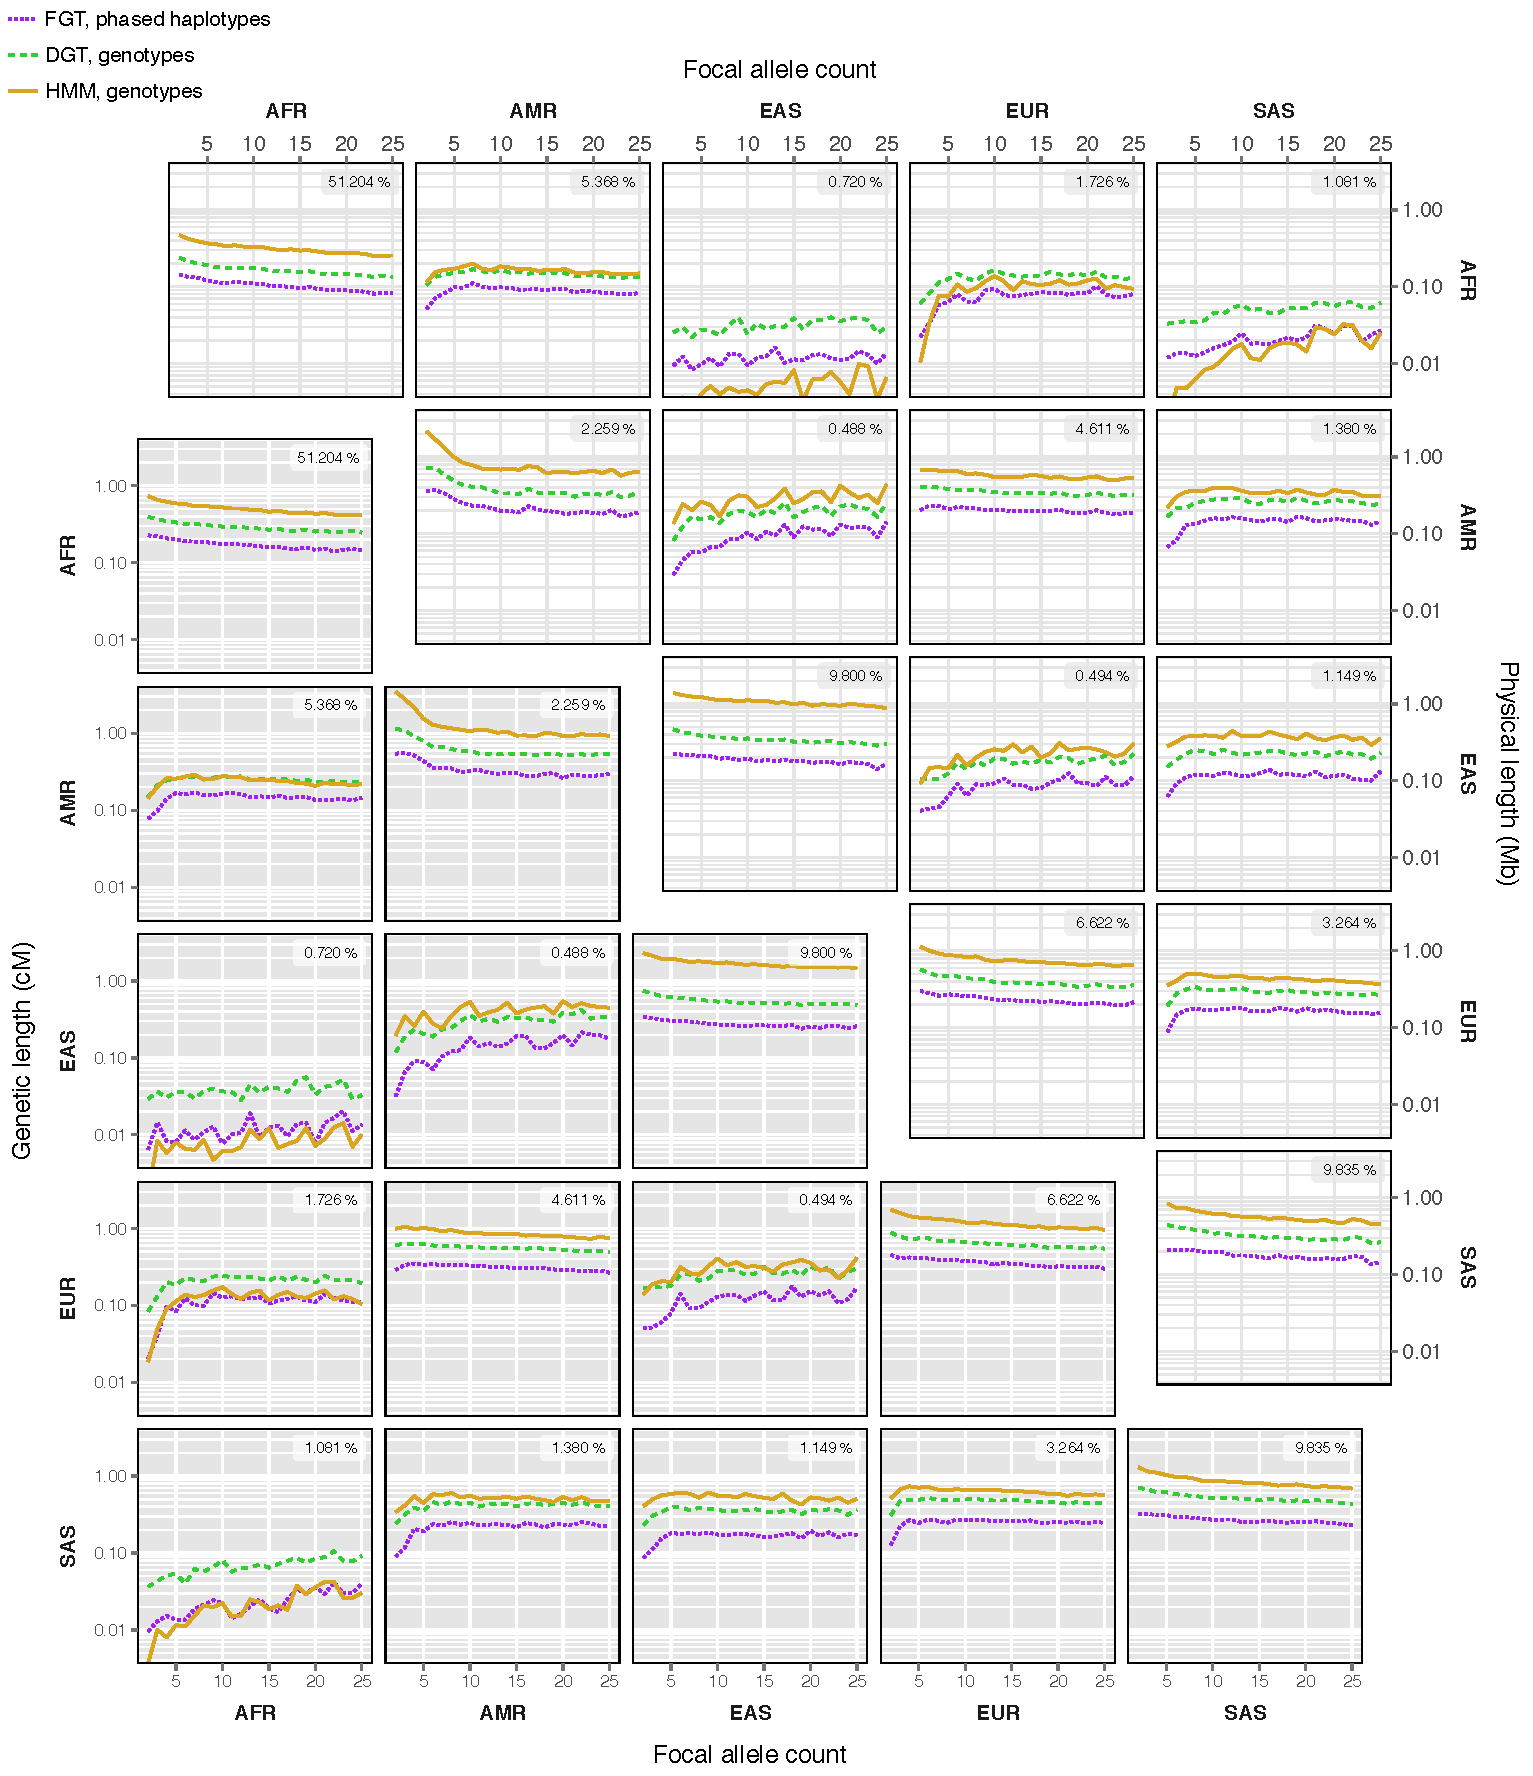
\includegraphics[width=1.1\textwidth]{./img/ch4/1KG_chr20_pop_len}%
}
\Caption{Inferred shared haplotype lengths by population in 1000 Genomes, chr.~20}
{The distributions of physical (upper triangle) and genetic (lower triangle) length by frequency of the focal allele are shown for alleles shared between pairs of individuals from the same population (\emph{diagonal} panels) and any of the other populations sampled in \gls{1kg}.
The \gls{1kg} Phase~\rom{3} dataset comprises samples from \n{5} continental populations (or \emph{super-populations});
African~(AFR), Ad-Mixed American~(AMR), East~Asian~(EAS), European~(EUR), and South~Asian~(SAS).
Results are shown for shared haplotype lengths inferred using the \gls{fgt}, \gls{dgt}, and \gls{hmm}, on the same set of segments inferred at target sites found at \fk{[2,25]} (\ie allele frequency below 0.5\%).
The proportion of haplotypes shared within or between each population is given in each panel (upper right corner).}
{fig:1KG_chr20_pop_len}
\end{figure}

%

Since IBD is delimited by past recombination events that occurred independently along each lineage back in time, the length of a shared haplotype region is indicative for the time since a haplotype was co-inherited from a common ancestor.
It is therefore expected that IBD segments are longer within a given population than segments shared between individuals from different populations.
I further subdivided the set of IBD segments based on the focal allele being shared between individuals from the same or different populations, as recorded in \gls{1kg}.
\Ctref{fig:1KG_chr20_pop_len} shows the distribution of median physical and genetic IBD length by focal allele frequency for each case, which also includes the results obtained using the \gls{fgt} and \gls{dgt}, where segments were detected on the same target site and haplotype pair.
\Ctref{tab:1kg20_pop_len} gives the overall median lengths for each comparison (sharing within and between populations).

%
% !TEX root = ../../main.tex


\begin{table}[!htb]
\Caption{Median shared haplotype length per population in 1000 Genomes, chromosome~20}
{Shared haplotype segments found around alleles shared within and between populations, as contained within \gls{1kg}.
The \gls{1kg} Phase~\rom{3} dataset comprises samples from \n{5} continental populations (or \emph{super-populations});
African~(AFR), Ad-Mixed American~(AMR), East~Asian~(EAS), European~(EUR), and South~Asian~(SAS).
The results shown compare median physical and genetic lengths of segments detected using \gls{fgt}, \gls{dgt}, and \gls{hmm}.
Shared haplotypes inferred around alleles shared within the same population are marked ($\ast$).}
{tab:1kg20_pop_len}
\centering
\begin{tabular}{cccc*3{S[table-format=1.3]}c*3{S[table-format=1.3]}}
\toprule
\multicolumn{3}{c}{Populations} & &
\multicolumn{3}{c}{Physical length (Mb)} & &
\multicolumn{3}{c}{Genetic length (cM)} \\
\cmidrule(lr){5-7}
\cmidrule(lr){9-11}
 & & & &
 \multicolumn{1}{c}{\textsc{fgt}} &
 \multicolumn{1}{c}{\textsc{dgt}} &
 \multicolumn{1}{c}{\textsc{hmm}} &
 &
 \multicolumn{1}{c}{\textsc{fgt}} &
 \multicolumn{1}{c}{\textsc{dgt}} &
 \multicolumn{1}{c}{\textsc{hmm}} \\
\midrule
AFR & $\ast$ & AFR   & &   0.0953630  &  0.1538850  &  0.2935880   & &   0.16057776  &  0.27368286  &  0.47134933 \\
AFR &        & AMR   & &   0.0883050  &  0.1441820  &  0.1601910   & &   0.14693635  &  0.24837901  &  0.23652881 \\
AFR &        & EAS   & &   0.0115740  &  0.0315790  &  0.0050850   & &   0.01156149  &  0.03785932  &  0.00813254 \\
AFR &        & EUR   & &   0.0774200  &  0.1368035  &  0.1024660   & &   0.11410845  &  0.21700701  &  0.12844471 \\
AFR &        & SAS   & &   0.0208440  &  0.0515020  &  0.0172550   & &   0.02374001  &  0.07137431  &  0.02252322 \\
AMR & $\ast$ & AMR   & &   0.2038830  &  0.3557680  &  0.7129400   & &   0.31137054  &  0.57153883  &  1.08905972 \\
AMR &        & EAS   & &   0.1028560  &  0.1969615  &  0.2942145   & &   0.15574224  &  0.31515857  &  0.42889480 \\
AMR &        & EUR   & &   0.1967920  &  0.3374810  &  0.5530320   & &   0.30437058  &  0.54800974  &  0.83130167 \\
AMR &        & SAS   & &   0.1470260  &  0.2606995  &  0.3443815   & &   0.22954635  &  0.42494642  &  0.50971107 \\
EAS & $\ast$ & EAS   & &   0.1810310  &  0.3371910  &  1.0471060   & &   0.26898801  &  0.53432077  &  1.65876398 \\
EAS &        & EUR   & &   0.0852165  &  0.1712245  &  0.2273470   & &   0.11975636  &  0.25972257  &  0.29546667 \\
EAS &        & SAS   & &   0.1150430  &  0.2235760  &  0.3671295   & &   0.16811773  &  0.35266527  &  0.52353278 \\
EUR & $\ast$ & EUR   & &   0.2208935  &  0.3799455  &  0.7222260   & &   0.34646435  &  0.61871972  &  1.13196026 \\
EUR &        & SAS   & &   0.1640040  &  0.2876520  &  0.4199520   & &   0.25448201  &  0.46803180  &  0.61850847 \\
SAS & $\ast$ & SAS   & &   0.1722970  &  0.3115490  &  0.5513870   & &   0.26487589  &  0.51306615  &  0.83429636 \\
\bottomrule
\end{tabular}
\end{table}

%

The length of segments inferred around alleles shared within the same population decreased towards higher allele frequencies and were generally longer compared to haplotypes shared between a given population and any of the others.
Such expected differences were more pronounced for results obtained using the HMM.
While the \gls{fgt} and \gls{dgt} overall resulted in shorter detected haplotype segments, the HMM was able to infer even shorter segments;
for example, see haplotype sharing between African~(AFR) and East~Asian~(EAS) individuals in \cref{fig:1KG_chr20_pop_len}.
Further, note that the effect of error on the \gls{fgt} and \gls{dgt} would be reduced at shorter IBD segments, as it becomes less likely to encounter false positive breakpoints.


It should be noted that different values of \Ne would apply to the different populations.
The results shown here were obtained from the analysis on the full \gls{1kg} sample, where $\Ne=\n{10000}$ was used as model parameter in the HMM.
The effect of using different values of \Ne, which is one of the parameters in the computation of transition probabilities, would need further evaluation.
Also, recall that the emission probabilities used here were derived from data simulated using $\Ne=\n{7300}$, which may further impact the accuracy of inference.
Such possible variations, however, were treated as negligible here, as it appeared more relevant to first demonstrate the general feasibility of the proposed method.




%
\subsection{Discussion}
%

The analysis on simulated data has shown that the HMM-based approach to infer IBD around target sites is able to operate equally well in both absence and presence of error.
In particular, I showed that IBD segments detected using the HMM maintained high levels of accuracy when genotype error was present.
However, a notable caveat is seen in the decreasing accuracy towards higher frequencies of the focal allele; for example, IBD segments identified by \fk{2} variants were overall higher in accuracy compared to \fk{15} or higher

A possible explanation could be that the emission model was generated under the assumption of recent IBD, where the empirical distributions closely followed the expected genotype pair frequencies \Addition{where it was assumed that no further mutations occur on a co-inherited haplotype.}
\Addition{For example, as given in \ctref{eq:genpairibd}, the expected probability to observe genotype pair $g_{02}$ or $g_{20}$ in \emph{ibd} would be equal to zero.
While this assumption may hold true for very recent co-inheritance, and perhaps under the convenient conditions of simulation, it is easily violated in reality.
The empirical model provided a more realistic approximation to observing genotype pairs in real data (as well as simulated data), but was still limited to observations made under recent co-inheritance.}

To have a more complete picture of the differences in the probability of observing each possible genotype pair, I again used the simulation records to sample IBD segments that were co-inherited at varying points in time.
The resulting empirical probability distributions are dependent on the allele frequency at the site of a given genotype pair and the \gls{tmrca} of the underlying shared haplotype, which is shown in \cpref{fig:emission_tmrca}, both before and after error.
For example, at \gls{tmrca}$\leq1$, the rate at which genotype pair $g_{02}$ or $g_{20}$ was observed was zero throughout before error, but non-zero after error.
But, notably, differences due to error were subdued at older relationships.

%
% !TEX root = ../../main.tex


\begin{figure}[!htb]
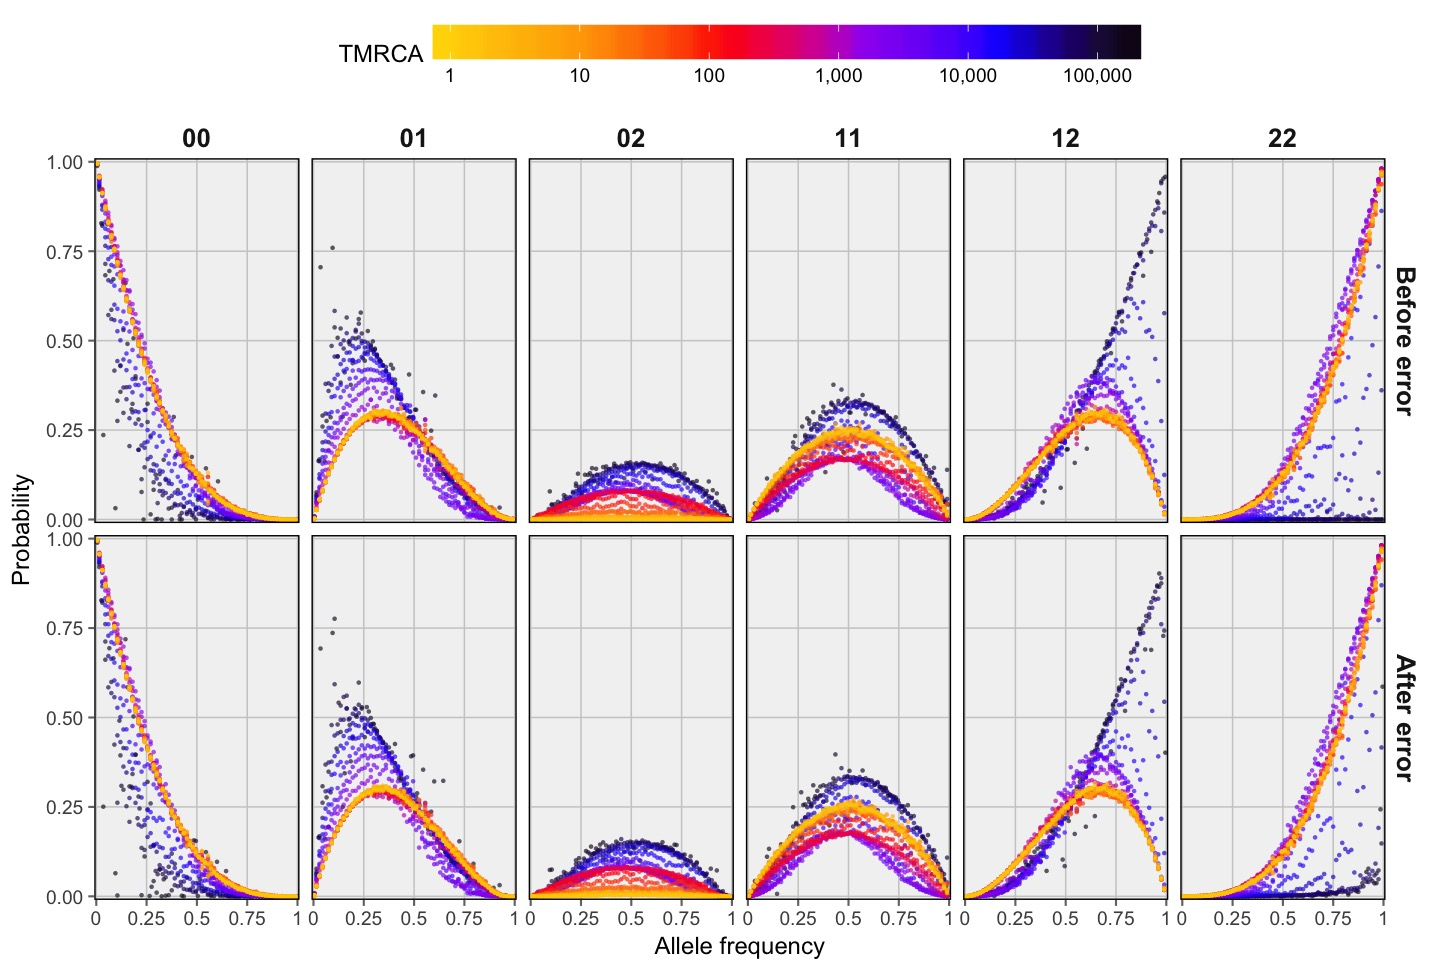
\includegraphics[width=\textwidth]{./img/ch4/emission_tmrca_reduced_new}
\Caption{Empirical emission probabilities of genotype pairs observed at different T\textsubscript{MRCA}}
{The relative proportions of genotype pairs observed in IBD segments are distinguished by \glsentryfull{tmrca} for a given pair of haplotypes, which was derived from simulation records.
The datasets used to obtain the empirical distributions before and after error were the original, error-free and the error-treated dataset, respectively; see \cpref{sec:create_error_data}.
IBD segments were sampled at 50 time intervals equally spaced on log-scale.
Observation rates of genotype pairs were calculated per allele frequency bin, defined on equal steps of 1\%.}
{fig:emission_tmrca}
\end{figure}

%


\Addition{One caveat of the HMM-based method is its reliance on genotype data.
It is possible that there may be several, similar recently co-inherited shared haplotypes involved, whose combined effects on the observed genotype frequency distribution is not straightforward to distinguish based on observations from genotype data alone.
The analysis of the simulated dataset and its tree structure has suggested that there was little overlap of recently co-inherited IBD segments on average for a pair of diploid individuals.
However, this observation cannot be generalised as it would be expected that the underlying shared haplotype structure is affected by population stratification and other demographic parameters such as inbreeding and geographic isolation of a population.}


\Addition{Another consideration is that focal allele frequency may not be an ideal indicator for allele age or, in particular, \gls{tmrca}.
The HMM-based method uses the expected age of the target allele observed at a given frequency to modulate the transition probability from the focal \emph{ibd} state to the \emph{non} state.
This approximation could be regarded as being unsuitable, because the expected length of an IBD segment is dependent in \gls{tmrca} and where the actual age of an allele within a given segment may only be informative if that allele derived from a mutation event around the time of the MRCA of the two haplotypes involved.
For example, it would be expected that the majority of shared alleles within the interval of a recent and relatively long segment are (much) older than the time since co-inheritance of that segment.
However, recall that I attempted to minimise such confounders in the current analysis by removing ``duplicate'' segments, where only the segment found around the target allele with the lowest frequency was retained per pair.}


\Addition{Lastly, it must be noted that the results obtained from the analysis of \gls{1kg} data are likely to be confounded due to false allele sharing.
In presence of data error, not all observed shared alleles correctly identify a recently co-inherited shared haplotype, which is particularly problematic towards lower allele frequencies; for example, see }\cpref{fig:fk_error}\Addition{.
Future analyses may therefore consider to only analyse focal alleles that were called or typed with high confidence.}




%
%%% Replaced with above
%
% Besides data error, the accumulation of mutations over time are expected to lead to further deviations from expectations under IBD.
%
% The difference between recent and older relationships of IBD is exemplified in \cpref{fig:emission_tmrca}, where I used the same methodology I applied as in \cpref{sec:HMMError}, using the error-free dataset ($D$), but where I distinguished IBD segments by \gls{tmrca}.
% The difference is shown between IBD haplotypes that were very recently co-inherited (\gls{tmrca}$<10$ generations) and those denoting older relationships (\gls{tmrca}$\geq \num{10000}$ generations).
% The resulting proportions of genotype pairs, \ie their observation probability dependent on age,
% show an interesting pattern, but one that may be difficult to model.
% For example, $g_{0 0}$ and $g_{2 2}$ genotype pairs appear to be consistent and less variable most of the time, but then show a distribution as expected under non-IBD at very old age ($\geq \num{10000}$ generations).
% In contrast, the $g_{0 2}$ genotype pair gradually increases from zero probability expected under IBD to a distribution expected under non-IBD.
% Interestingly, the $g_{1 1}$ genotype pair varies inconsistently with regard to either expectation at intermediate time frames (\eg between \n{1000} and \n{10000} generations).
% This result suggests that a static emission model may not provide sufficient leverage to distinguish IBD from non-IBD at older (\ie higher-frequency) alleles, or in general when IBD is not recent.
% It would therefore be advantageous to device a fully probabilistic model to compute emission probabilities; \eg conditional on mutation rate and expected allele age, similar to the transition model.
%



% Conversely, their length distribution is likely to affect the inference of the breakpoint interval around the focal \fk{}~variant.

% The directionality of the process limits the inference of separate IBD segments.
% For example, if the allele frequency of shared alleles at other positions in the sequence would be considered, the Markov assumption of retrospective state dependence would not hold any longer.

% Second, \glspl{hmm} typically exhibit an exponential complexity dependent on the number of states.
% Although the state space, $S$, of the presented model is small, the whole sequence needs to be traversed in order to infer only the focal segment.
% This makes computation of thousands of focal sites impractical.
% In a left-to-right model, the process length of the Markov chain can be reduced by including a stop condition, \eg


%
%\subsection{Comparison to 1000 Genomes data}
%


% One possible explanation for
% lies within the centromere.
% Although simulations were performed using a variable recombination rate according to a genetic map from the \gls{hapmap},


% 1KG, linear regression: FGT DGT HMM
% FGT, phased haplotypes.A. Physical length 0.234074 0.0007438657
% DGT, genotypes.A. Physical length 0.4071223 -0.001372566
% HMM, genotypes.A. Physical length 1.29611 -0.03788508
% FGT, phased haplotypes.B. Genetic length 0.5961899 -0.01083166
% DGT, genotypes.B. Genetic length 1.151849 -0.02689706
% HMM, genotypes.B. Genetic length 2.980023 -0.1062093


%
%\section{Discussion}
%


% reasons why there still is a discrepancy between expectations and inferred segment lengths in 1000G
% may be due to falsely called alleles, with increasing error rates towards to lower frequencies.
% other than removing suspiciously short segments
% there is no direct way of detecting such false positives.
% biological processes not considered in the simulation
